\documentclass[../notes.tex]{subfiles}

\pagestyle{main}
\renewcommand{\chaptermark}[1]{\markboth{\chaptername\ \thechapter\ (#1)}{}}

\begin{document}




\chapter{Structure Determination}
\section{Intro + Elemental Analysis}
\begin{itemize}
    \item \marginnote{9/4:}Teaching team.
    \begin{itemize}
        \item Prof. Masha Elkin.
        \item Prof. Steve Buchwald.
        \item 8 Teaching Fellows (TFs).
    \end{itemize}
    \item Masha Elkin begins. Steve Buchwald and all TFs introduce themselves. Special roles:
    \begin{itemize}
        \item Head TF: Minh Le.
        \item Electronic TF (contact with questions on Canvas, Piazza, BACON): Angel Garcia-Ramirez.
    \end{itemize}
    \item In this class, you will learn\dots
    \begin{itemize}
        \item New things in organic chemistry;
        \item Old things at a deeper level;
        \item Real-world applications of chemistry.
    \end{itemize}
    \item Why study organic chemistry?
    \begin{itemize}
        \item Chemists manipulate matter, and that's awesome!
        \item By "manipulate matter," we mean making molecules, breaking molecules, making polymers, making detergents, and making sure that all of these things break down in the environment :)
    \end{itemize}
    \item Core questions.
    \begin{itemize}
        \item \emph{How} do we make molecules?
        \item What molecules \emph{should} we make?
    \end{itemize}
    \item Course logistics.
    \begin{itemize}
        \item Seven (7) units total (2 big units before the halfway mark \& 5 smaller units after).
        \item The units.
        \begin{itemize}
            \item Unit 1: How do we know what molecule(s) we have?
            \item Unit 2: How do electrons move?
            \item Units 3-7: How do we make molecules? How do reactions work?
        \end{itemize}
        \item Exams after units 1, 2, 4, and 6; final exam after unit 7.
        \item Questions? Ask your TF first, then the Head TF, then the profs (Masha \& Steve).
    \end{itemize}
    \item Prerequisites.
    \begin{itemize}
        \item Official prerequisites: 5.12 (equivalent to Orgo I, in case you took it elsewhere) \& Gen Chem.
        \item Recommended reading for review: Chapters 1-2 of the main textbook, referred to in these notes as \textcite{bib:Clayden}.
    \end{itemize}
    \item Grading.
    \begin{itemize}
        \item Your grade will (hopefully) be a reflection of your learning.
        \item There are no curves in this class or at MIT, so \emph{everyone can get an A!!!}
        \item How to improve your grade: Do problems!
        \begin{itemize}
            \item Problem sets (PSets) and recitation worksheets will be provided.
            \item You may also do as many textbook problems as you want. Feel free to buy the solutions manual, or borrow a copy from the ChemEd office\footnote{Located in 6-203.} to check your answers.
        \end{itemize}
    \end{itemize}
    \item How to learn organic chemistry.
    \begin{itemize}
        \item Analogy: Learning Orgo is like learning a language.
        \begin{itemize}
            \item Basic vocab and grammar that must be memorized. Examples: Drawing structures, curved arrow formalism, etc.
            \item Recognizing patterns and trends. Examples: Nucleophiles tend to have lone pairs (or be other regions of high electron density).
            \item Developing intuition.
            \item Practice, practice, practice! (Focus on drawing structures.)
        \end{itemize}
        \item Tips for success.
        \begin{itemize}
            \item Be active and participate in lecture, recitation, etc. Take notes while you're here!
            \item Practice \textbf{metacognition}, i.e., learn how you learn.
            \begin{itemize}
                \item Do you learn best in a crowded coffee shop, or in your own room? Would you rather recopy your notes, or read the textbook?
                \item Note that what works for somebody else may not work for you, and vice versa!
                \item Invest the time and effort that \emph{you} need to succeed. This may be more (or less) than other students, and that's ok!
            \end{itemize}
            \item Communicate with \emph{the whole} teaching team. They're here to help!!!
            \begin{itemize}
                \item Seek out accommodations as needed: It's the student's responsibility to ask.
            \end{itemize}
        \end{itemize}
    \end{itemize}
    \item \textbf{Metacognition}: Being aware of your own understanding.
    \item We now begin the content for Unit 1.
    \item Goal: Learn how to determine the chemical structure of a given organic compound.
    \item Why do we need to determine structures?
    \begin{figure}[h!]
        \centering
        \begin{tikzpicture}
            \begin{scope}[xshift=-1cm,scale=0.4]
                \fill [gaz] (-0.5,0) -- (-1,-1) -- (1,-1) -- (0.5,0);
                \draw [gay,thick,decorate,decoration={snake,segment length=4pt,amplitude=0.5pt}] (-0.5,0) -- (0.5,0);
    
                \draw [gray,ultra thick] (-0.3,1) -- (-0.3,0.5) -- (-1,-1) -- (1,-1) -- (0.3,0.5) -- (0.3,1);
            \end{scope}
            \draw [thick,-latex] (-0.4,0) -- (0.4,0);
            \node at (1.1,0) {\chemfig[atom sep=1.4em]{*6(-=-=-=)}};
        \end{tikzpicture}
        \caption{Why we study structure determination.}
        \label{fig:structureDeterminationRationale}
    \end{figure}
    \begin{itemize}
        \item With the naked eye, organic chemists see a flask with a colorless liquid. But we draw the skeletal diagram for benzene (which is a colorless liquid). What tools enable us to convert from the flask to the structure?
        \item Here's another reason: Suppose we run a brand new chemical reaction. Organic chemists do this all the time in research! How do we now what the product is? How do we know which atoms it contains, and in what arrangement?
    \end{itemize}
    \item Structure determination workflow.
    \begin{enumerate}
        \item Identify the atoms present.
        \begin{itemize}
            \item Questions to answer: What is the molecular formula?
            \item Relevant tools: Elemental analysis (EA) and mass spectrometry ("mass spec" or MS).
        \end{itemize}
        \item Identify the functional groups and substructures present.
        \begin{itemize}
            \item Questions to answer: Do we have ketones? Esters? Alcohols? Rings?
            \item Relevant tools: MS, infrared spectroscopy (IR), and nuclear magnetic resonance (NMR).\footnote{NMR is an organic chemist's best friend!}
        \end{itemize}
        \item Identify how all the functional groups fit together.
        \begin{itemize}
            \item Questions to answer: Are they close? Far apart? Ortho/meta/para? What stereochemistry?
            \item Relevant tools: NMR and X-ray diffraction.
        \end{itemize}
    \end{enumerate}
    \item We now begin talking about EA.
    \begin{itemize}
        \item History: Began development in the 1820s.
        \item Purpose: Determine which elements are present, and in what quantities (in a given sample).
    \end{itemize}
    \item In this course, we will apply EA to compounds containing carbon, hydrogen, and oxygen \emph{exclusively}.
    \begin{itemize}
        \item To reiterate, in an EA problem for this course, we will \emph{not} have to worry about any other elements.
        \item The typical EA technique for such compounds is \textbf{combustion analysis}.
    \end{itemize}
    \item \textbf{Combustion analysis}: Burn the sample and measure the products.
    \begin{itemize}
        \item All \ce{C} in the sample becomes \ce{CO2}.
        \item All \ce{H} in the sample becomes \ce{H2O}.
        \item \ce{O} is then determined via process of elimination, explained as follows.
    \end{itemize}
    \item Advanced techniques (beyond the scope of this class): Nitrogen to \ce{NO} or \ce{NO2}, sulfur to \ce{SO2}, etc.
    \item A schematic of combustion analysis.
    \begin{figure}[h!]
        \centering
        \begin{tikzpicture}
            \footnotesize
            \filldraw [draw=brown,thick,fill=brown!20] (0,-0.18) ellipse (2mm and 1mm);
            \node at (0,0.8) {Sample}
                edge[bend right=10,->] (0,0)
            ;
            \node at (0,-0.8) {\ce{CuO}}
                edge[bend right=10,->] (0.5,-0.1)
            ;
    
            \fill [gaz] (1.4,-1)
                -- ({1.4+0.24},-1)
                arc[start angle=-140,end angle=-40,x radius=0.73cm,y radius=1.12cm]
                -- ({1.4+1.6},-1)
                arc[start angle=-40,end angle=-140,x radius=1.04cm,y radius=1.66cm]
                -- cycle
            ;
            \draw [gay,thick,decorate,decoration={snake,segment length=4pt,amplitude=0.5pt}] (1.4,-1) -- (1.64,-1);
            \draw [gay,thick,decorate,decoration={snake,segment length=4pt,amplitude=0.5pt}] (2.76,-1) -- (3,-1);
            \node at (2.2,-2.1) {\ce{CaCl2}}
                edge[bend right=10,->] (2.2,-1.45)
            ;
            \fill [gaz] (3.5,-1)
                -- ({3.5+0.24},-1)
                arc[start angle=-140,end angle=-40,x radius=0.73cm,y radius=1.12cm]
                -- ({3.5+1.6},-1)
                arc[start angle=-40,end angle=-140,x radius=1.04cm,y radius=1.66cm]
                -- cycle
            ;
            \draw [gay,thick,decorate,decoration={snake,segment length=4pt,amplitude=0.5pt}] (3.5,-1) -- ({3.5+0.24},-1);
            \draw [gay,thick,decorate,decoration={snake,segment length=4pt,amplitude=0.5pt}] ({3.5+1.6-0.24},-1) -- ({3.5+1.6},-1);
            \node at (4.3,-2.1) {\ce{KOH}}
                edge[bend right=10,->] (4.3,-1.45)
            ;
    
            \draw
                (-1.2,0) ellipse (0.5mm and 1mm)
                (-1.2,0.1)  -- (-0.7,0.1)
                (-1.2,-0.1) -- (-0.7,-0.1)
                (-0.7,-0.3) rectangle (0.7,0.3)
                (0.7,-0.1) -- (1.2,-0.1)
                    arc[start angle=-180,end angle=0,x radius=1cm,y radius=1.5cm]
                    -- ++(0.1,0)
                    arc[start angle=-180,end angle=0,x radius=1cm,y radius=1.5cm]
                    -- ++(0.3,0)
                (0.7,0.1) -- (1.38,0.1)
                    arc[start angle=-180,end angle=0,x radius=0.82cm,y radius=1.5cm]
                    -- ++(0.46,0)
                    arc[start angle=-180,end angle=0,x radius=0.82cm,y radius=1.5cm]
                    -- ++(0.48,0)
                (5.6,0) ellipse (0.5mm and 1mm)
            ;
            \node at (-2,0) {\ce{O2}}
                edge [->] (-1.4,0)
            ;
            \node at (6.4,0) {\ce{O2}}
                edge [<-] (5.8,0)
            ;
        \end{tikzpicture}
        \caption{Combustion analysis schematic.}
        \label{fig:schematicEA}
    \end{figure}
    \begin{itemize}
        \item Burn the sample in the presence of an oxidant such as cupric oxide (\ce{CuO}).
        \item Flow \ce{O2} into the combustion chamber to facilitate burning as well.
        \item The combusted gas then flows through a series of reaction containers.
        \begin{itemize}
            \item The first one contains a desiccant (like \ce{CaCl2}) that absorbs the water.
            \item The second one contains a base (like \ce{KOH}) that absorbs the \ce{CO2}.
        \end{itemize}
        \item The remaining oxygen flows out the end.
    \end{itemize}
    \item The \emph{analysis} part of combustion analysis.
    \begin{itemize}
        \item The amount of \ce{H} is equal to the change in mass of the \ce{CaCl2}.
        \begin{equation*}
            \Delta\text{mass}(\ce{CaCl2}) = \text{mass}(\ce{H2O})
            \to \text{ratio}(\ce{H})
        \end{equation*}
        \item The amount of \ce{C} is equal to the change in mass of the \ce{KOH}.
        \begin{equation*}
            \Delta\text{mass}(\ce{KOH}) = \text{mass}(\ce{CO2})
            \to \text{ratio}(\ce{C})
        \end{equation*}
        \item The amount of \ce{O} is equal to the change in mass of the sample.
        \begin{equation*}
            \text{mass}(\text{sample})-\text{mass}(\ce{H})-\text{mass}(\ce{C}) = \text{mass}(\ce{O})
             \to \text{ratio}(\ce{O})
        \end{equation*}
        \item Result: We get an \textbf{empirical formula} of the form \ce{C_{$x$}H_{$y$}O_{$z$}}. Remember that this is \emph{not} (necessarily) the \textbf{molecular formula}; it is \emph{only} a ratio of elements.
    \end{itemize}
    \item EA example: Let's burn \SI{0.5}{\gram} of propanol (\ce{C3H8O}).
    \begin{itemize}
        \item Suppose we obtain \SI{0.600}{\gram} \ce{H2O} and \SI{1.09}{\gram} \ce{CO2}.
        \item This means that there was \SI{0.067}{\gram} (\ce{H}) and \SI{0.300}{\gram} (\ce{C}) in the sample. The remaining \SI{0.133}{\gram} must then be due to \ce{O}.
        \item Therefore, the elements exist in a 3:8:1 (C:H:O) ratio.
        \item Bonus: Convert the masses to a ratio via stoichiometry.
        \begin{itemize}
            \item $
                \SI{0.600}{\gram}\ \ce{H2O}
                \times\dfrac{\SI{1}{\mole}\ \ce{H2O}}{\SI{18.02}{\gram}\ \ce{H2O}}
                \times\dfrac{\SI{2}{\mole}\ \ce{H}}{\SI{1}{\mole}\ \ce{H2O}}
                \times\dfrac{\SI{1.01}{\gram}\ \ce{H}}{\SI{1}{\mole}\ \ce{H}}
                = \SI{0.067}{\gram}\ (\ce{H})
            $
            \item $
                \SI{1.09}{\gram}\ \ce{CO2}
                \times\dfrac{\SI{1}{\mole}\ \ce{CO2}}{\SI{44.01}{\gram}\ \ce{CO2}}
                \times\dfrac{\SI{1}{\mole}\ \ce{C}}{\SI{1}{\mole}\ \ce{CO2}}
                \times\dfrac{\SI{12.01}{\gram}\ \ce{C}}{\SI{1}{\mole}\ \ce{C}}
                = \SI{0.300}{\gram}\ (\ce{C})
            $
            \item $
                \SI{0.5}{\gram}\ \text{propanol}
                -\SI{0.067}{\gram}\ (\ce{H})
                -\SI{0.300}{\gram}\ (\ce{C})
                = \SI{0.133}{\gram}\ (\ce{O})
            $
        \end{itemize}
    \end{itemize}
    \item A note on the previous example.
    \begin{table}[h!]
        \centering
        \small
        \renewcommand{\arraystretch}{1.4}
        \begin{tabular}{l|cc|ccc}
            \textbf{Name} & Propanol & Methyl ethyl ether & Formaldehyde & Acetic acid & Glucose\\
            \textbf{Structure} &
                \footnotesize\chemfig[atom sep=1em]{-[:30]-[:-30]-[:30]OH} &
                \footnotesize\chemfig[atom sep=1em]{-[:30]-[:-30]O-[:30]} &
                \footnotesize\chemfig[atom sep=1em,baseline=1.2em]{H-[:30](=[2]O)-[:-30]H} &
                \footnotesize\chemfig[atom sep=1em,baseline=0.65em]{-[:30](=[2]O)-[:-30]OH} &
                \footnotesize\chemfig[atom sep=1em,baseline=-0.4em]{?(-[:190]HO)-[:-50,1.4](-[:170]HO)-[:10,1.5](-[:-55]OH)-[:-10,1.5](-[:10]OH)-[:130]O-[:190]?(-[:150,0.7]-[2]OH)}\\
            \textbf{Emp. formula} & \ce{C3H8O} & \ce{C3H8O} & \ce{CH2O} & \ce{CH2O} & \ce{CH2O}\\
            \textbf{Mol. formula} & \ce{C3H8O} & \ce{C3H8O} & \ce{CH2O} & \ce{C2H4O2} & \ce{C6H12O6}\\
        \end{tabular}
        \caption{Questions that EA can't answer.}
        \label{tab:EAmols}
    \end{table}
    \begin{itemize}
        \item EA has given us the empirical formula, but it has \emph{not} confirmed that the sample is propanol. For example, methyl ethyl ether has the same empirical formula!
        \item Additionally, we don't yet have the molecular formula. Consider, for instance, the breadth of compounds with empirical formula \ce{CH2O}!
        \item Takeaway: EA gives you the empirical formula; we need MS to get the molecular formula (we'll see this on Friday), and we may need even more to get the atomic connectivity.
    \end{itemize}
    \item Application of EA to real-world chemistry.
    \begin{itemize}
        \item A home furnace burns natural gas --- which is mostly methane (\ce{CH4}) --- for heat.
        \item \textbf{Ideal combustion}\footnote{You can learn more about in a chemical engineering/ChemE course.} corresponds to the reaction
        \begin{equation*}
            \ce{CH4 + O2 -> CO2 + H2O}
        \end{equation*}
        \item Real-world combustion is incomplete; you make
        \begin{equation*}
            \ce{CH4 + air -> CO2 + H2O + NO2 + CO}
        \end{equation*}
        \item When a technician comes to your home, they analyze the flue gas (i.e., your furnace exhaust).
        \begin{itemize}
            \item Their analysis could determine that our combustion has too much \ce{O2}, which is called "air rich." This is inefficient and doesn't yield enough heat.
            \item They could also determine that you have too much \ce{CO2} and \ce{CO}, which is called "fuel rich." This yields too much soot and \ce{CO}. \ce{CO} can be dangerous and lead to carbon monoxide poisoning, which makes you sleepy before it kills you.
        \end{itemize}
        \item To measure this flue gas, though, they have a little handheld elemental analysis device!
    \end{itemize}
    \item Note that there is a relation between ideal/real-world combustion and the \ce{CuO} oxidant in Figure \ref{fig:schematicEA}: The \ce{CuO} ensures that when we combust our EA sample, all the carbon is fully oxidized to \ce{CO2}! Without it, some \ce{CO} would be formed, and our stoichiometry would be thrown off.
\end{itemize}



\section{Mass Spectrometry}
\begin{itemize}
    \item \marginnote{9/6:}Lecture 1 recap.
    \begin{itemize}
        \item Elemental analysis (EA).
        \begin{equation*}
            \ce{SM + O2 ->[$\Delta$] CO2 + H2O}
        \end{equation*}
        \begin{itemize}
            \item SM means "\underline{s}tarting \underline{m}aterial."
            \item SM's we will focus on: Compounds of the form \ce{C_{$x$}H_{$y$}O_{$z$}}.
        \end{itemize}
        \item Empirical formula vs. molecular formula (see Table \ref{tab:EAmols}).
    \end{itemize}
    \item Today: Mass spectrometry (MS).
    \begin{itemize}
        \item Purpose: Convert empirical formulas to molecular formulas (and more!).
        \item Reading: \textcite{bib:Clayden}, Chapter 3.
    \end{itemize}
    \item Lecture outline.
    \begin{itemize}
        \item Mass spectrometer schematic.
        \item Mass spectrum elements.
        \item Fragmentation, and common types.
        \item Isotope effects in MS.
        \item Ionization methods.
    \end{itemize}
    \item \textbf{Mass spectrometry}: A structure determination technique that tells us the exact mass of molecules and their "fragments." \emph{Also known as} \textbf{MS}, "\textbf{mass spec}."
    \item Overview.
    \begin{center}
        \schemestart
        \chemfig{\cnc{M}}
        \arrow{-U>[\footnotesize$\textup{e}^-$][\footnotesize$2\textup{e}^-$]}
        \chemfig{\charge{20=\scriptsize +,-3=$\cdot$}{\cnc{M}}}
        \arrow(M--b)
        \subscheme{
            \chemfig{\charge{12=\scriptsize +}{\cnc{M$-b$}}}
            \+{3mm}
            \chemfig{\charge{[extra sep=1pt]30=$\cdot$}{\cnc{$b$}}}
        }
        \arrow(--a){0}[90,0.1]
        \subscheme{
            \chemfig{\charge{12=\scriptsize +}{\cnc{M$-a$}}}
            \+{3mm}
            \chemfig{\charge{[extra sep=1pt]30=$\cdot$}{\cnc{$a$}}}
        }
        \arrow(@b--c){0}[-90,0.1]
        \subscheme{
            \chemfig{\charge{12=\scriptsize +}{\cnc{M$-c$}}}
            \+{3mm}
            \chemfig{\charge{[extra sep=1pt]30=$\cdot$}{\cnc{$c$}}}
        }
        \arrow(@M--@a.west)
        \arrow(@M--@c.west)
        \schemestop
    \end{center}
    \begin{itemize}
        \item You have a sample --- denoted by $\cnc{M}$ --- that you bombard with electrons ($\e[-]$). When an electron hits a molecule of your sample, it knocks off one of the molecule's electrons (and flies off itself). This ionizes your molecule to a \textbf{radical cation}, denoted by $\cnc{M}\rc$ and called the \textbf{molecular ion}.
        \item This radical cation is unstable and fragments into a proper cation and a proper radical. The radical is usually not detected, but any cationic fragment produced --- the $\cnc{M$-a$}^+$, $\cnc{M$-b$}^+$, and $\cnc{M$-c$}^+$ above --- usually \emph{is} detected.
    \end{itemize}
    \item A (stepwise) schematic of a mass spectrometer.
    \begin{figure}[h!]
        \centering
        \footnotesize
        \begin{tikzpicture}
            \fill [gray!70,rotate around={-10:(2.3,0)}] (1.8,-0.8)
                -- node[below=1mm,black,digit]{5} (2.8,-0.8)
                -- (2.8,0.6)
                -- (1.8,0.6)
            ;
            \fill [white] (-0.3,0.1)
                -- (0,0.1)
                -- (0,0.5)
                -- (1.5,0.5)
                arc[start angle=90,end angle=35,radius=4cm]
                -- ++(-145:1)
                arc[start angle=35,end angle=90,radius=3cm]
                -- (0,-0.5)
                -- (0,-0.1)
                --(-0.3,-0.1)
            ;
    
            \draw [decorate,decoration={coil,segment length=2.2pt},rotate around={180:(0.4,0.4)}] (0.1,0.4) -- node[above=2mm,digit]{2} (0.7,0.4);
    
            \draw (0.2,-0.5)
                -- (0.2,-0.9)
                -- node[below=1mm,digit]{3} (0.5,-0.9)
                -- (0.5,-0.5)
            ;
            \draw [-stealth] (0.35,-0.45) -- ++(0,0.23);
            \draw [-stealth] (0.42,-0.45) -- ++(0.12,0.16);
            \draw [-stealth] (0.28,-0.45) -- ++(-0.12,0.16);
    
            \draw
                (-0.3,0) ellipse (0.3mm and 1mm)
                (-0.3,0.1) -- (0,0.1)
                    -- (0,0.5)
                    -- (1.5,0.5)
                    arc[start angle=90,end angle=35,radius=4cm] coordinate (b) node[right=1mm,digit]{6}
                (-0.3,-0.1) -- (0,-0.1)
                    -- (0,-0.5)
                    -- (1.5,-0.5)
                    arc[start angle=90,end angle=35,radius=3cm] coordinate (a) %node[left=2mm,digit]{6}
            ;
            \draw
                (1,0.5) arc[start angle=90,end angle=-90,x radius=1mm,y radius=5mm]
                (1.3,0.5) arc[start angle=90,end angle=-90,x radius=1mm,y radius=5mm]
                (0.9,0.02)  -- ++(0.2,0)
                (0.9,-0.02) -- ++(0.2,0)
                (1.2,0.02)  -- ++(0.2,0)
                (1.2,-0.02) -- ++(0.2,0)
            ;
            \draw
                (1,0.5) arc[start angle=90,end angle=270,x radius=1mm,y radius=5mm]
                (1.3,0.5) arc[start angle=90,end angle=270,x radius=1mm,y radius=5mm]
            ;
            \node [below,digit] at (1.15,-0.6) {4};
            \draw [rotate=-55] ($(a)!0.5!(b)+(0,0.5)$) arc[start angle=90,end angle=-90,x radius=1mm,y radius=5mm];
            \draw [rotate=-55] ($(a)!0.5!(b)+(0,0.5)$) arc[start angle=90,end angle=270,x radius=1mm,y radius=5mm];
    
            \node [label={[above,digit]1}] at (-1.8,0) {Sample}
                edge [dashed,->] (-0.45,0)
            ;
            \draw [dashed,->] (-0.1,0) -- (0.85,0);
            \draw [dashed,->] (1.45,0)
                -- (1.5,0)
                arc[start angle=90,end angle=49,radius=1.9cm] %node[circle,fill,inner sep=1pt]{}
                -- ++({49-90}:1.65)
            ;
            \draw [dashed,->] (1.45,0)
                -- (1.5,0)
                arc[start angle=90,end angle=57,radius=2.3cm] %node[circle,fill,inner sep=1pt]{}
                -- ++({57-90}:1.8)
            ;
            \draw [dashed,->] (1.45,0)
                -- (1.5,0)
                arc[start angle=90,end angle=63,radius=2.8cm] %node[circle,fill,inner sep=1pt]{}
                -- ++({63-90}:1.93)
            ;
        \end{tikzpicture}
        \caption{Mass spectrometer schematic.}
        \label{fig:schematicMS}
    \end{figure}
    \begin{enumerate}
        \item The sample is injected into a curved tube.
        \item A heater vaporizes the sample.
        \item An electron source (also known as an electron gun) shoots electrons at the vaporized sample, ionizing it. The ionized sample starts fragmenting.
        \item The fragments encounter a series of negatively charged plates with slits in the middle. These negatively charged plates accelerate the positively charged cations.
        \item A magnet deflects the accelerated, positively charged ions. The magnet deflects them based on their \textbf{mass-to-charge ratio}. Because of physics, the lightest ions are deflected the most, and the heaviest ions are deflected the least.
        \item A detector records where the ions hit. This data is converted into a mass-to-charge ratio for each ion. This yields a spectrum of all the fragments' masses.
    \end{enumerate}
    \item \textbf{Mass-to-charge ratio} (of a cation): The cation's mass divided by its net charge. \emph{Denoted by} $\bm{m/z}$.
    \begin{itemize}
        \item For the purposes of this class, $z=1$.
    \end{itemize}
    \item Example mass spectrum: Acetone (\,{\tiny\chemfig[baseline=1mm,atom sep=1em,bond offset=1pt,fixed length=false]{-[:30](=[2]O)-[:-30]}}\,).
    \begin{figure}[H]
        \centering
        \begin{tikzpicture}[xscale=0.16,yscale=0.04]
            \small
            \node [rotate=90] at (-5.875,50) {Relative Intensity};
            \node [below=5mm] at (35,0) {$m/z$};
    
            \footnotesize
            \draw (-0.625,100) node[left]{$100$} -- ++(1.125,0);
            \foreach \x in {10,20,...,60} {
                \draw (\x,2.5) -- ++(0,-5) node[below]{$\x$};
            }
    
            \draw [orange,ultra thick]
                (15,0) -- ++(0,14) node[above=1mm,black,thin,digit]{15} node[above=6mm,black]{$\cnc{M$-43$}^+=\cnc{CH3}^+$}
                (27,0) -- ++(0,1)
                (28,0) -- ++(0,1)
                (29,0) -- ++(0,1)
                (43,0) -- ++(0,100) node[above=1mm,black,thin,digit]{43} node[above=6mm,black]{${}^{\color{white}+}\cnc{M$-15$}^+=[\chemfig[atom sep=1.4em,fixed length=false,bond sep=2pt]{H_3C-~O}]^+$}
                (44,0) -- ++(0,3)
                (58,0) -- ++(0,26) node[above=1mm,black,thin,digit]{58} node[above=6mm,black]{${}^{\color{white}+}\cnc{M}\rc=\Big[{\tiny\chemfig[baseline=1.3mm,atom sep=1em,bond offset=1pt,fixed length=false]{-[:30](=[2]O)-[:-30]}}\Big]{}^\rc$}
                (59,0) -- ++(0,2)
            ;
    
            \draw (0,110) -- (0,0) -- (70,0);
        \end{tikzpicture}
        \vspace{-0.5em}
        \caption{Mass spectrum of acetone.}
        \label{fig:MSacetone}
    \end{figure}
    \begin{itemize}
        \item The $x$-axis is the mass-to-charge ratio, and the $y$-axis is the "relative intensity" of each peak.
        \begin{itemize}
            \item If a certain fragment gets produced more than another (and hence recorded more than it), we say it has a "higher relative intensity."
        \end{itemize}
        \item We identify two special types of peaks in a mass spectrum: The \textbf{parent peak} and the \textbf{base peak}. In the case of acetone\dots
        \begin{itemize}
            \item The parent peak lies at 58;
            \item The base peak lies at 43.
        \end{itemize}
        \item The peak at 15 also has a relatively large magnitude, and from the fact that the mass of a methyl cation is approximately 15, we can infer that this peak corresponds to the methyl cation fragment.
        \begin{itemize}
            \item Notice that its intensity is significantly lower than the intensity of the base peak because we may recall from Orgo I that the methyl cation is a far less stable cation than the resonance-stabilized, secondary acylium ion at 43.
        \end{itemize}
        \item There are a number of smaller peaks, too, but they give less information.
        \item Note that the major peaks may be appropriately referred to by \emph{any} of the three nomenclature methods in Figure \ref{fig:MSacetone}: By exact mass, by $\cnc{M$-a$}^+$, and/or by structure.
    \end{itemize}
    \item \textbf{Parent peak}: The peak in a mass spectrum corresponding to the molecular ion.
    \begin{itemize}
        \item The parent peak is always the rightmost peak in the spectrum.\footnote{Excepting isotope effects; discussed later in this lecture.} This is because it is created by the heaviest ion, and you can't have more mass than your initial molecule!
        \item It is typically \emph{not} the tallest peak in the spectrum.
        \item Useful information: It gives the molecular weight of the molecule.
    \end{itemize}
    \item \textbf{Base peak}: The tallest peak in a mass spectrum.
    \begin{itemize}
        \item The base peak corresponds to the fragment that the molecule forms most preferentially, which is usually also the most stable fragment.
    \end{itemize}
    \item \textbf{Fragmentation peak}: Any peak to the left of the parent peak.
    \item Maxim: Molecules fragment in predictable ways to form stable cations.
    \item At this point, let's formally define \textbf{fragmentation}.
    \item \textbf{Fragmentation}: The formation of stable(-ish) cations.
    \begin{itemize}
        \item Recall from Orgo I (review your notes on cation stability!!) that stable cations tend to be more substituted, delocalized, atom-stabilized (e.g., close to a heteroatom), etc. 
    \end{itemize}
    \item Let's now discuss some common species that we analyze via MS --- and how they fragment.
    \item Alkane fragmentation: Preferentially break bonds to get more substituted (e.g., $2^\circ$ \& $3^\circ$) carbocations.
    \item Example: Isopentane (\,{\tiny\chemfig[baseline=0.8mm,atom sep=1em,bond offset=1pt,fixed length=false]{-[:30](-[2])-[:-30]-[:30]}}\,).
    \begin{figure}[H]
        \centering
        \footnotesize
        \setchemfig{atom sep=1.4em}
        \schemestart
            \chemfig{-[:30](-[@{1}2])-[@{2}:-30]-[:30]}
            \arrow(--.174)
            \chemname{
                \chemleft[
                    \chemfig{-[:30](-[2])-[:-30]-[:30]}
                \chemright]
            }{$m/z=72$\\parent (minor)}
            \+{,,2mm}
            \chemname{
                \chemleft[
                    \chemfig{-[:30]\charge{[extra sep=5pt]90=$\oplus$}{}(-[2,,,,opacity=0])-[:-30]-[:30]}
                \chemright]
            }{$m/z=57$\\(major)}
            \+{,,2mm}
            \chemname{
                \chemleft[
                    \chemfig{-[:30]\charge{[extra sep=4pt]-30=$\oplus$}{}(-[2])-[:-30,,,,opacity=0]}
                \chemright]
            }{$m/z=43$\\(major)}
            \arrow{0}[,0.1]\+{,,2.5em}\arrow(--.165){0}[0,0.1]
            \chemname[1.2em]{
                \chemleft[
                    \chemfig{Et}
                \chemright]
            }{$m/z=29$\\(minor)}
            \arrow{0}[,0.1]\+{,,3.43em}\arrow{0}[0,0.1]
            \chemname[1.2em]{
                \chemleft[
                    \chemfig{Me}
                \chemright]
            }{$m/z=15$\\(minor)}
        \schemestop
        \hspace{-2mm}
        \chemmove{
            \draw [-,rex] ($(1)+(180:0.18)$) node[circle,draw,fill=white,inner sep=1pt]{} -- ($(1)+(0:0.18)$) node[circle,draw,fill=white,inner sep=1pt]{};
            \draw [-,rex] ($(2)+(-120:0.18)$) node[circle,draw,fill=white,inner sep=1pt]{} -- ($(2)+(60:0.18)$) node[circle,draw,fill=white,inner sep=1pt]{};
        }
        \begin{tikzpicture}[remember picture,overlay]
            % \draw (-13,0.37) -- ++(13,0);
            % \draw (-13,-0.19) -- ++(13,0);
            \node at (-8.82,0.65) {\tiny$\rc$};
            \node at (-1.96,0.38) {${}^+$};
            \node at (0,0.38) {${}^+$};
        \end{tikzpicture}
        \caption{Fragmentation of alkanes.}
        \label{fig:fragAlkane}
    \end{figure}
    \begin{itemize}
        \item All these peaks will appear, but the tallest will correspond to the species labeled "major" above.
    \end{itemize}
    \item Alcohol fragmentation.
    \begin{itemize}
        \item Dehydration: Yields an $\cnc{M$-18$}^+$ peak, corresponding to the loss of water.
        \item $\alpha$-cleavage: Leads to a resonance-stabilized product.
    \end{itemize}
    \item Example: Pentan-3-ol (\,{\tiny\chemfig[baseline=1mm,atom sep=1em,bond offset=1pt,fixed length=false]{(-[:150])-[:30](-[2]OH)-[:-30]-[:30]}}\,).
    \begin{figure}[h!]
        \centering
        \footnotesize
        \setchemfig{atom sep=1.4em}
        \begin{subfigure}[b]{0.49\linewidth}
            \centering
            \schemestart
                \chemname{
                    \chemfig{-[:-30]-[:30](-[@{1}2]OH)-[:-30]-[:30]}
                }{$m/z=88$}
                \arrow
                \chemname{
                    \chemleft[
                        \chemfig{-[:-30]-[:30](-[2,,,,opacity=0]\phantom{OH})=_[:-30]-[:30]}
                    \chemright{]^+}
                }{$m/z=70$}
            \schemestop
            \chemmove{
                \draw [-,rex] ($(1)+(180:0.18)$) node[circle,draw,fill=white,inner sep=1pt]{} -- ($(1)+(0:0.18)$) node[circle,draw,fill=white,inner sep=1pt]{};
            }
            \caption{Dehydration.}
            \label{fig:fragOHa}
        \end{subfigure}
        \begin{subfigure}[b]{0.49\linewidth}
            \centering
            \schemestart
                \chemname{
                    \chemfig{-[:-30]-[:30](-[2]OH)-[@{2}:-30]-[:30]}
                }{$m/z=88$}
                \arrow
                \chemname{
                    \chemleft[\subscheme{
                        \chemfig{-[:-30]-[:30]\charge{[extra sep=4pt]-30=$\oplus$}{}-[2]OH}
                        \arrow{<->}
                        \chemfig{-[:-30]-[:30]=^[2]\charge{[extra sep=4pt]180=$\oplus$}{O}H}
                    }\chemright]
                }{$m/z=59$}
            \schemestop
            \chemmove{
                \draw [-,rex] ($(2)+(-120:0.18)$) node[circle,draw,fill=white,inner sep=1pt]{} -- ($(2)+(60:0.18)$) node[circle,draw,fill=white,inner sep=1pt]{};
            }
            \caption{$\alpha$-cleavage.}
            \label{fig:fragOHb}
        \end{subfigure}
        \caption{Fragmentation of alcohols.}
        \label{fig:fragOH}
    \end{figure}
    \item Ketone fragmentation.
    \begin{itemize}
        \item $\alpha$-cleavage: Leads to a resonance-stabilized product, once again.
        \item McLafferty rearrangement: Only happens for ketones with a $\gamma$-proton.
        \begin{itemize}
            \item We select for this type of ketone because in this case, we can form a six-membered transition state. Recall that six-membered transition states are super stable in organic chemistry!
            \item This fragmentation leads to a charged enol (that we see in the spectrum) and an uncharged olefin (that we don't see in the spectrum).
        \end{itemize}
    \end{itemize}
    \item Example: Hexanones.
    \begin{figure}[h!]
        \centering
        \footnotesize
        \setchemfig{atom sep=1.4em}
        \begin{subfigure}[b]{\linewidth}
            \centering
            \schemestart
                \chemname{
                    \chemfig{(-[:-150])-[:-30]-[@{3}:30](=[2]O)-[@{2}:-30]-[:30]}
                }{$m/z=100$}
                \arrow(.11--.174)
                \chemname{
                    \chemleft[
                        \chemfig{(-[:-150])-[:-30]-[:30]~[:30]\charge{[extra sep=5pt]100=$\oplus$}{O}}
                    \chemright]
                }{$m/z=71$}
                \+
                \chemname{
                    \chemleft[
                        \chemfig{(~[:150]\charge{[extra sep=5pt]80=$\oplus$}{O})-[:-30]-[:30]}
                    \chemright]
                }{$m/z=57$}
            \schemestop
            \chemmove{
                \draw [-,rex] ($(2)+(-120:0.18)$) node[circle,draw,fill=white,inner sep=1pt]{} -- ($(2)+(60:0.18)$) node[circle,draw,fill=white,inner sep=1pt]{};
                \draw [-,rex] ($(3)+(-60:0.18)$) node[circle,draw,fill=white,inner sep=1pt]{} -- ($(3)+(120:0.18)$) node[circle,draw,fill=white,inner sep=1pt]{};
            }
            % \begin{tikzpicture}[remember picture,overlay]
            %     \draw (-5,0.88) -- ++(13,0);
            %     \draw (-5,0.32) -- ++(13,0);
            % \end{tikzpicture}
            \caption{$\alpha$-cleavage.}
            \label{fig:fragKetonea}
        \end{subfigure}\\[2em]
        \begin{subfigure}[b]{\linewidth}
            \centering
            \schemestart
                \chemfig{-[:30](=[2]O)-[:-30]\charge{[extra sep=4pt]-90=$\alpha$}{}-[:30]\charge{[extra sep=4pt]90=$\beta$}{}-[:-30]\charge{[extra sep=4pt]-90=$\gamma$}{}-[:30]}
                \arrow(--.170)
                \chemname[0em]{
                    \chemleft[
                        \chemfig[atom sep=2.5em,fixed length=false]{-[:30](=[@{db}2]O)-[@{sb2}:-30]-[@{sb3}:30]-[@{sb4}2](-[@{sb5}:150]H-[@{sb6,0.3}:-150,,,,opacity=0])-[:30]}
                    \chemright]
                }{$m/z=100$}
                \arrow(.10--.151)
                \chemname[1.5em]{
                    \chemleft[
                        \chemfig{-[:30](-[2]OH)=_[:-30]}
                    \chemright]
                }{$m/z=58$}
                \arrow(--.210){0}[,0]\+{,,3.9mm}
                \chemfig{=_[2]-[:30]}
            \schemestop
            \chemmove{
                \draw [curved arrow={2pt}{1pt},arrows={-Stealth[harpoon,flex]}] (db) to[out=10,in=-70,out looseness=2,in looseness=1] (sb6);
                \draw [curved arrow={2pt}{1pt},arrows={-Stealth[harpoon,flex,swap]}] (db) to[out=-10,in=70,out looseness=2,in looseness=1.5] (sb2);
                \draw [curved arrow={1pt}{1pt},arrows={-Stealth[harpoon,flex]}] (sb3) to[out=130,in=50,out looseness=2,in looseness=1.5] (sb2);
                \draw [curved arrow={1pt}{1pt},arrows={-Stealth[harpoon,flex,swap]}] (sb3) to[out=110,in=-170,out looseness=2,in looseness=1.5] (sb4);
                \draw [curved arrow={1pt}{1pt},arrows={-Stealth[harpoon,flex]}] (sb5) to[out=-110,in=170,out looseness=2,in looseness=1.5] (sb4);
                \draw [curved arrow={1pt}{1pt},arrows={-Stealth[harpoon,flex,swap]}] (sb5) to[out=-130,in=-50,out looseness=2,in looseness=1] (sb6);
            }
            \begin{tikzpicture}[remember picture,overlay]
                % \draw (-5,1.45) -- ++(13,0);
                % \draw (-5,0.32) -- ++(13,0);
                \node at (-4.24,1.08) {\tiny$\rc$};
                \node at (-1.12,0.8) {\tiny$\rc$};
            \end{tikzpicture}
            \caption{McLafferty rearrangement.}
            \label{fig:fragKetoneb}
        \end{subfigure}
        \caption{Fragmentation of ketones.}
        \label{fig:fragKetone}
    \end{figure}
    \item Isotope effects.
    \item Principle: Mass spectrometry weighs individual molecules, so molecules containing a heavier (or lighter) isotope will appear separate from other molecules in the mass spectrum.
    \item Atoms with notable isotope effects.
    \begin{figure}[H]
        \centering
        \begin{subfigure}[b]{0.17\linewidth}
            \centering
            \begin{tikzpicture}
                \draw [orange,ultra thick]
                    (0.8,0) -- ++(0,1.2)
                    (0.96,0) -- ++(0,0.05)
                ;

                \draw (0,1.4) -- (0,0) -- (1.8,0);
            \end{tikzpicture}
            \caption{Carbon.}
            \label{fig:isotopeEffectsMSa}
        \end{subfigure}
        \begin{subfigure}[b]{0.17\linewidth}
            \centering
            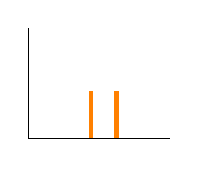
\begin{tikzpicture}
                \draw [orange,ultra thick]
                    (0.8,0) -- ++(0,0.6)
                    (1.12,0) -- ++(0,0.6)
                ;
                
                \draw (0,1.4) -- (0,0) -- (1.8,0);
            \end{tikzpicture}
            \caption{Bromine.}
            \label{fig:isotopeEffectsMSb}
        \end{subfigure}
        \begin{subfigure}[b]{0.17\linewidth}
            \centering
            \begin{tikzpicture}
                \draw [orange,ultra thick]
                    (0.8,0) -- ++(0,0.9)
                    (1.12,0) -- ++(0,0.3)
                ;
                
                \draw (0,1.4) -- (0,0) -- (1.8,0);
            \end{tikzpicture}
            \caption{Chlorine.}
            \label{fig:isotopeEffectsMSc}
        \end{subfigure}
        \caption{Isotope effects in MS.}
        \label{fig:isotopeEffectsMS}
    \end{figure}
    \begin{itemize}
        \item Carbon: The $\ce{{}^12C}:\ce{{}^13C}$ ratio is $99:1$.
        \begin{itemize}
            \item Implication: For every $\cnc{M}\rc$, we see 1\% $\cnc{M$+1$}\rc$.
            \item This is why we see tiny "shadow" peaks to the right of the parent peak and base peak in Figure \ref{fig:MSacetone}!
            \begin{itemize}
                \item Note that the "shadow" of the parent peak is 3\% its height (not 1\%) because there are \emph{three} carbons in the acetone molecular ion.
                \item Similarly, the "shadow" of the base peak is 2\% its height because there are \emph{two} carbons in the acylium ion.
            \end{itemize}
        \end{itemize}
        \item Bromine: The $\ce{{}^79Br}:\ce{{}^81Br}$ ratio is $1:1$.
        \begin{itemize}
            \item Implication: The $\cnc{M}\rc$ and $\cnc{M$+2$}\rc$ peaks exist in a $1:1$ ratio, i.e., have the same height/relative intensity.
            \item The splitting of the molecular ion peak into two such peaks is a super recognizable, distinct, and useful fingerprint of bromine-containing compounds!
        \end{itemize}
        \item Chlorine: The $\ce{{}^35Cl}:\ce{{}^37Cl}$ ratio is $3:1$.
        \begin{itemize}
            \item Implication: The $\cnc{M}\rc$ and $\cnc{M$+2$}\rc$ peaks exist in a $3:1$ ratio.
            \item Similar to bromine, this peak splitting is a fingerprint of chlorine-containing compounds.
        \end{itemize}
    \end{itemize}
    \item Combining everything we've learned up to this point, let's do another example.
    \item Example: Benzyl chloride (\,{\tiny\chemfig[baseline=0.5mm,atom sep=1em,bond offset=1pt,fixed length=false]{*6(=-=(--[:-30]Cl)-=-)}}\,).
    \begin{figure}[h!]
        \centering
        \begin{tikzpicture}[xscale=0.08,yscale=0.04]
            \small
            \node [rotate=90] at (-11.75,50) {Relative Intensity};
            \node [below=5mm] at (80,0) {$m/z$};
    
            \footnotesize
            \draw (-1.25,100) node[left]{$100$} -- ++(2.5,0);
            \foreach \x in {50,100,150} {
                \draw (\x,2.5) -- ++(0,-5) node[below]{$\x$};
            }
    
            \draw [orange,ultra thick]
                (40,0) -- ++(0,8) node[above=1mm,black,thin,digit]{40}
                (65,0) -- ++(0,12) node[above=1mm,black,thin,digit]{65}
                (91,0) -- ++(0,100) node[above=1mm,black,thin,digit,label={[right=2mm,yshift=-2mm,black]
                    \chemleft[
                        \chemfig[atom sep=1em]{*6(=-=(-\charge{[extra sep=5pt]90=$\oplus$}{})-=-)}
                    \chemright]
                }]{91}
                (92,0) -- ++(0,7) node[above right=1mm,black,thin,digit]{92}
                (126,0) -- ++(0,27) node[above=1mm,black,thin,digit,label={[right=2.5mm,yshift=2mm,black]
                    \chemleft[
                        \chemfig[atom sep=1em]{*6(=-=(--[:-30]{}^{35}Cl)-=-)}
                    \chemright{]^\rc}
                }]{126}
                (128,0) -- ++(0,9) node[above right=1mm,black,thin,digit,label={[right=2.5mm,yshift=-2mm,black]
                    \chemleft[
                        \chemfig[atom sep=1em]{*6(=-=(--[:-30]{}^{37}Cl)-=-)}
                    \chemright{]^\rc}
                }]{128}
            ;
    
            \draw (0,110) -- (0,0) -- (160,0);
        \end{tikzpicture}
        \vspace{-0.5em}
        \caption{Mass spectrum of benzyl chloride.}
        \label{fig:MSBnCl}
    \end{figure}
    \begin{itemize}
        \item The parent peak will lie at 126, and the corresponding chlorine isotope peak will lie at 128 and be one-third the height.
        \item The base peak will lie at 91, and the corresponding carbon isotope peak will lie at 92 and be 7\% the height (to account for the 7 carbons in the benzylic cation that may be heavy).
        \begin{itemize}
            \item It will correspond to the most stable fragment, which in this case is the benzylic cation.
            \item The benzylic cation is super stable because its positive charge can be resonance delocalized to four different atoms!
            \item A large peak at $m/z=91$ strongly suggests the presence of an aromatic system.
        \end{itemize}
        \item This example focused on predicting the peaks in a mass spectrum based on reasonable fragmentation patterns. But what if we are given the mass spectrum? What data can we pull out then?
    \end{itemize}
    \item To answer this question, here are some guidelines for the interpretation of mass spectra.
    \item Guidelines for interpretation.
    \begin{itemize}
        \item The parent peak provides the molecular weight of the molecule.
        \begin{itemize}
            \item This allows you to convert an empirical formula obtained from EA to the molecular formula.
        \end{itemize}
        \item The parent peak also reveals key atoms via distinct isotopic fingerprints.
        \begin{itemize}
            \item Examples include bromine and chlorine.
            \item An additional one is the \textbf{nitrogen rule}.
        \end{itemize}
        \item Fragmentation patterns can identify substructures.
        \begin{itemize}
            \item Recall from Lecture 1 (9/4) that identifying substructures is part of the second step of the structure determination workflow!
            \item Common fragments:
            \begin{itemize}
                \item Loss of a methyl group is $-15$.
                \item Loss of an OH group is $-17$.
                \item Loss of \ce{H2O} is $-18$.
                \item Loss of \ce{CO2} is $-44$.
                \item Loss of a \ce{{}^$t$Bu} group is $-57$.
            \end{itemize}
            \item Look at the $m/z$ of the fragments \emph{and} the difference in $m/z$ between certain fragments.
            \begin{itemize}
                \item Example: Maybe a certain fragment is formed by losing both a methyl group \emph{and} water.
            \end{itemize}
        \end{itemize}
        \item Important note: These guidelines are just a guide; we will need multiple forms of evidence to support an assignment.
    \end{itemize}
    \item \textbf{Nitrogen rule}: If you have an odd number of nitrogen in a molecule, you will get an odd molecular weight.
    \begin{itemize}
        \item The basis for this rule lies in the fact that nitrogen is trivalent but has an even mass.
        \begin{itemize}
            \item This means that nitrogen tends to bond an odd number of groups (specifically, 3), making the overall mass odd.
        \end{itemize}
        \item Examples: Ammonia has an odd mass of $17=14+1+1+1$ and methylamine has an odd mass of $31=(14+1+1)+(12+1+1+1)$, while methane has an even mass of $16=12+1+1+1+1$ and ethane has an even mass of $30=(12+1+1+1)+(12+1+1+1)$.
        \item You can read more about the nitrogen rule \href{https://en.wikipedia.org/wiki/Nitrogen_rule}{here}.
        \item Implication: If you see an odd molecular weight, you \emph{might} have a nitrogen present!
    \end{itemize}
    \item Types of ionization.
    \item \textbf{Electron ionization}: A beam of electrons. \emph{Denoted by} \textbf{EI}. \emph{Also known as} \textbf{hard ionization}.
    \begin{itemize}
        \item This is the method we are using in this class.
    \end{itemize}
    \item \textbf{Electrospray ionization}: Forms charged droplets. \emph{Denoted by} \textbf{ESI}. \emph{Also known as} \textbf{soft ionization}.
    \begin{itemize}
        \item ESI causes less fragmentation.
        \item One implication of this is that you observe a larger parent peak.
        \item Another consequence is that ESI can analyze a broader range of compounds via mass spectrometry than EI can, since some sensitive compounds (like proteins) would never survive an electron beam.
        \begin{itemize}
            \item Nobel Prize in Chemistry (2002) for this application of MS to biology!
        \end{itemize}
    \end{itemize}
    \item \textbf{High resolution mass spectrometry}. \emph{Denoted by} \textbf{HRMS}.
    \begin{itemize}
        \item In "normal" low-resolution mass spectrometry (LRMS), both \ce{N2} and \ce{C2H4} have $m/z=28$.
        \item In HRMS, \ce{N2} has $m/z=28.0061$ and \ce{C2H4} has $m/z=28.0314$.
    \end{itemize}
    \item HRMS leads nicely into our application for today!
    \item Application of MS to real-world chemistry: Isotopic signatures.
    \begin{itemize}
        \item Today, you learned that the $\ce{{}^12C}:\ce{{}^13C}$ ratio is $99:1$.
        \begin{itemize}
            \item In reality, this is an \emph{average} value.
            \item The actual ratio of isotopes is globally uneven, and we as humans have mapped it.
        \end{itemize}
        \item Indeed, isotope abundances vary by time and location due to air patterns, etc.
        \item For example, Montana is home to 2\% more \ce{{}^13C} than Florida!
        \item Implication: We can tell if a narcotic is made in the US (and where) or another country based on the isotopic abundance in it.
        \item We can also track where a person, drug, or uranium sample is from.
        \begin{itemize}
            \item Naturally, the government is very interested in this technology :)
        \end{itemize}
        \item You can also tell if a person eats corn or rice because this leads to different ratios of nitrogen isotopes in our bodies.
    \end{itemize}
\end{itemize}



\section{Infrared Spectroscopy}
\begin{itemize}
    \item \marginnote{9/9:}Lecture 2 recap.
    \begin{itemize}
        \item In mass spectrometry, you ionize your sample $\cnc{M}$ to the molecular ion $\cnc{M}\rc$.
        \item $\cnc{M}\rc$ is detected as the parent peak.
        \begin{itemize}
            \item The parent peak provides the molecular weight (MW) of the molecule.
            \item The parent peak also reveals any isotopic signatures.
        \end{itemize}
        \item Many molecular ions --- once formed --- will fragment into cations $\cnc{M$-a$}^+$, $\cnc{M$-b$}^+$, $\cnc{M$-c$}^+$, etc.
        \begin{itemize}
            \item More stable cations are formed more often, resulting in higher relative intensities.
            \item The \emph{most} stable fragment gives rise to the base peak.
        \end{itemize}
        \item Common fragments include those resulting from\dots
        \begin{itemize}
            \item The loss of a methyl group;
            \item The loss of a water molecule;
            \item $\alpha$-cleavage;
            \item The McLafferty rearrangement (for ketones).
        \end{itemize}
    \end{itemize}
    \item Today: Infrared Spectroscopy (IR).
    \begin{itemize}
        \item Reading: \textcite{bib:Clayden}, Chapter 3.
        \item Prof. Elkin highly recommends the section on IR; be sure to read this!!
    \end{itemize}
    \item Lecture outline.
    \begin{itemize}
        \item Spectrometer schematic.
        \item Theory.
        \item Spectrum elements.
        \item Key regions of a spectrum.
    \end{itemize}
    \item Principle: Irradiate a sample with infrared waves and detect where the sample absorbs these waves.
    \begin{itemize}
        \item This technique is useful for identifying certain functional groups, namely those that absorb IR waves well.
    \end{itemize}
    \pagebreak
    \item A schematic of an infrared spectrometer.
    \begin{figure}[h!]
        \centering
        \footnotesize
        \begin{tikzpicture}
            \node [draw,minimum height=9mm] {IR source};
    
            \node at (3,0) {\chemfig[atom sep=1.4em]{-[:15,0.75](=[2]O)-[:-45,0.8]}};
            \draw (2.6,-0.5) -- node[below=3mm]{Sample} ++(0.8,-0.3) -- ++(0,1.4) -- ++(-0.8,0.3) -- cycle;
    
            \draw (5.7,0) ellipse (5mm and 8mm) node[below=9.5mm]{Detector};
    
            \draw [rex,semithick,-latex,decorate,decoration={snake,amplitude=1.5pt,segment length=5pt,post length=1.5mm}] (0.8,0.3) -- ++(0.5,0);
            \draw [rex,semithick,-latex,decorate,decoration={snake,amplitude=1.5pt,segment length=7pt,post length=1.5mm}] (0.8,0.1) -- ++(0.8,0);
            \draw [rex,semithick,-latex,decorate,decoration={snake,amplitude=1.5pt,segment length=9pt,post length=1.5mm}] (0.8,-0.1) -- ++(1.1,0);
            \draw [rex,semithick,-latex,decorate,decoration={snake,amplitude=1.5pt,segment length=11pt,post length=1.5mm}] (0.8,-0.3) -- ++(1.4,0);
    
            \draw [rex,semithick,-latex,decorate,decoration={snake,amplitude=1.5pt,segment length=5pt,post length=1.5mm}] (3.5,0.3) -- ++(0.5,0);
            \draw [rex,semithick,-latex,decorate,decoration={snake,amplitude=1.5pt,segment length=7pt,post length=1.5mm}] (3.5,0.1) -- ++(0.8,0);
            \draw [rex,semithick,-latex,decorate,decoration={snake,amplitude=1.5pt,segment length=11pt,post length=1.5mm}] (3.5,-0.3) -- ++(1.4,0);
        \end{tikzpicture}
        \caption{Infrared spectrometer schematic.}
        \label{fig:schematicIR}
    \end{figure}
    \begin{itemize}
        \item We begin with a source of infrared radiation. This source shoots waves at our sample, which could be a molecule like acetone. The IR waves that the source emits have a range of frequencies.
        \item The sample will absorb certain frequencies, and the frequencies that are not absorbed are detected by a detector. In other words, the director detects the \textbf{transmittance} of the sample.
    \end{itemize}
    \item \textbf{Transmittance}: How much of each frequency of radiation passes through the sample.
    \item IR theory.
    \begin{figure}[h!]
        \centering
        \footnotesize
        \begin{subfigure}[b]{0.25\linewidth}
            \centering
            \begin{tikzpicture}
                \node (1) at (0,0) [circle,draw=blx,fill=blz,thick] {$m_1^{}$};
                \node (2) at (2,0) [circle,draw=grx,fill=grz,thick] {$m_2^{}$}
                    edge [decorate,decoration={snake,segment length=6.8pt}] (1)
                ;
            \end{tikzpicture}
            \caption{Springy bonds.}
            \label{fig:IRtheorya}
        \end{subfigure}
        \begin{subfigure}[b]{0.25\linewidth}
            \centering
            \begin{tikzpicture}
                \node (1) at (0,0) [circle,draw=gax,fill=gaz,thick] {\phantom{$m_1^{}$}};
                \node (2) at (2,0) [circle,draw=gax,fill=gaz,thick] {\phantom{$m_1^{}$}}
                    edge [decorate,decoration={snake,segment length=6.8pt}] (1)
                ;
    
                \draw [->] (0.25,0.5) -- ++(-0.5,0);
                \draw [->] (1.75,0.5) -- ++(0.5,0);
            \end{tikzpicture}
            \caption{Stretch.}
            \label{fig:IRtheoryb}
        \end{subfigure}
        \begin{subfigure}[b]{0.25\linewidth}
            \centering
            \begin{tikzpicture}
                \node (1) at (-1.25,0) [circle,draw=gax,fill=gaz,thick] {\phantom{$m_1^{}$}}
                    edge [shorten <=2pt,bend right=10,->,thin] (-0.5,-0.3)
                ;
                \node (2) at (0,0.7) [circle,draw=gax,fill=gaz,thick] {\phantom{$m_1^{}$}}
                    edge [decorate,decoration={snake,segment length=6.8pt}] (1)
                ;
                \node (3) at (1.25,0) [circle,draw=gax,fill=gaz,thick] {\phantom{$m_1^{}$}}
                    edge [decorate,decoration={snake,segment length=6.8pt}] (2)
                    edge [shorten <=2pt,bend left=10,->,thin] (0.5,-0.3)
                ;
            \end{tikzpicture}
            \caption{Bend.}
            \label{fig:IRtheoryc}
        \end{subfigure}
        \caption{Infrared spectroscopy theory.}
        \label{fig:IRtheory}
    \end{figure}
    \begin{itemize}
        \item Fundamental assumption: A chemical bond is like a spring between atoms.
        \begin{itemize}
            \item Recall from Gen Chem that in science, we often call a spring a \textbf{harmonic oscillator}. If you don't quite remember this term, review your Gen Chem notes or Google it!!
        \end{itemize}
        \item Let's dive a bit deeper into this analogy: Imagine we have two different atoms of masses $m_1,m_2$ joined by a "spring," as in Figure \ref{fig:IRtheorya}.
        \begin{itemize}
            \item Just like a real spring, chemical bonds can vibrate in different ways: They can stretch and contract (as in Figure \ref{fig:IRtheoryb}), bend (as in Figure \ref{fig:IRtheoryc}), etc.
            \item All of these different motions are called the \textbf{vibrational modes} of the chemical bonds.
        \end{itemize}
        \item Bonds absorb energy from IR waves when the frequency ($\nu$) of the IR wave matches the frequency of the stretching/bending motion.
        \begin{itemize}
            \item In other words, when you hit the resonance frequency, you absorb energy.
            \item This absorption of energy is detected as the loss of transmittance.
        \end{itemize}
        \item The change in energy between vibrational modes is related to characteristics of the bond as follows.
        \begin{equation*}
            \Delta E \approx \sqrt{\frac{k(m_1+m_2)}{m_1m_2}}
        \end{equation*}
        \begin{itemize}
            \item $k$ is the force constant (proportional to the bond strength).
            \item $m$ is the mass of atom 1 or 2.
            \item Implication: Stronger bonds (i.e., those with larger values of $k$) require more energy (i.e., higher $\nu$ IR waves) to absorb.
            \item Implication: Lighter atoms (i.e., those with lower values of $m$) require more energy (i.e., higher $\nu$ IR waves) to absorb.
        \end{itemize}
        \item One additional requirement: The chemical bond must have a dipole in order to absorb IR waves.
        \begin{itemize}
            \item Example: \ce{C#O} absorbs because \ce{O} is more electronegative than \ce{C}, but \ce{N#N} does not.
        \end{itemize}
    \end{itemize}
    \pagebreak
    \item Questions on IR theory.
    \begin{itemize}
        \item Why do bonds absorb energy \emph{only} when the frequency of the IR waves matches the frequency of the bond's vibration?
        \begin{itemize}
            \item The answer to this question is beyond the scope of the class, but Prof. Elkin gives the quantum mechanical explanation.
            \item Essentially, when a chemical bond absorbs energy, it gets excited to a higher-energy vibrational mode, which we may think of as a more intense vibration.
            \item However, because vibrational modes are separated by a set amount of energy, lower energy photons won't have enough energy to make it to the next vibrational mode while higher energy photons will provide too much energy to reach anything stable.
        \end{itemize}
        \item Why don't bonds without dipoles absorb IR waves?
        \begin{itemize}
            \item The explanation is also quantum mechanical, and hence also beyond the scope of this class.
            \item Essentially, symmetric bonds and molecules lack something called a dipole moment, and zero dipole moment zeroes out the absorption in the math of quantum mechanics. 
            \item Note that there is some really cool math and physics underlying the answer to this question, and Prof. Elkin recommends you look it up if you're interested!!
            \item In organic chemistry, however, we're more interested in what we can do with IR spectroscopy than in \emph{exactly} how it works. Essentially, for this class, you should learn how it works well enough to make sense of the trends in spectrum interpretation presented in this lecture, but you don't need to go deeper than that for now.
        \end{itemize}
        \item Why do lighter atoms require more energy? It seems like it would take more energy to push around a heavier atom.
        \begin{itemize}
            \item Check out the explanation in \textcite{bib:Clayden}; it's pretty comprehensive and understandable.
        \end{itemize}
    \end{itemize}
    \item Example IR spectrum: Propionic acid (\,{\tiny\chemfig[baseline=-0.5mm,atom sep=1em,bond offset=1pt,fixed length=false]{-[:-30]-[:30](=[2]O)-[:-30]OH}}\,).
    \begin{figure}[h!]
        \centering
        \begin{tikzpicture}[text height=1.5ex,text depth=0.25ex,xscale=1]
            \small
            \draw (0,4) -- node[rotate=90,above=6mm]{Transmittance (\%)} (0,0) -- node[below=4.7mm]{$\nu$ (\si{\per\centi\meter})} (14,0);
    
            \draw [|-]  (0 ,-1.9) -- node[below=1mm,draw]{\ce{X-H}} ++(6,0);
            \draw [|-]  (6 ,-1.9) -- node[below=1mm,draw]{$sp$} ++(2,0);
            \draw [|-]  (8 ,-1.9) -- node[below=1mm,draw]{\ce{X=Y}} ++(2,0);
            \draw [|-|] (10,-1.9) -- node[below=1mm,draw]{single bonds} ++(4,0);
    
            \footnotesize
            \node [below] at (0,0) {4000};
            \draw (2,0.1)  -- ++(0,-0.1) node[below]{3500};
            \draw (4,0.1)  -- ++(0,-0.1) node[below]{3000};
            \draw (6,0.1)  -- ++(0,-0.1) node[below]{2500};
            \draw (8,0.1)  -- ++(0,-0.1) node[below]{2000};
            \draw (10,0.1) -- ++(0,-0.1) node[below]{1500};
            \draw (12,0.1) -- ++(0,-0.1) node[below]{1000};
            \draw (14,0.1) -- ++(0,-0.1) node[below]{500};
            \draw (0,3.5) -- ++(-0.1,0) node[left]{100};
    
            \draw [<-] (0,-0.6) -- node[below=3mm,align=center]{Higher $E$\\(stronger bonds)} ++(2.3,0);
            \draw [<-] (14,-0.6) -- node[below=3mm,align=center]{Lower $E$\\(weaker bonds)} ++(-2.3,0);
    
            \draw [rex,semithick,decorate,decoration={random steps,segment length=2pt,amplitude=0.8pt},/pgf/fpu/install only={reciprocal}] (0,3.5)
                -- ++(2.5,0)
                to[out=0,in=180,out looseness=0.4,in looseness=0.5] ++(1,-1.7) node[black,above=1.7cm]{\ce{O-H}}
                to[out=0,in=180,out looseness=0.6,in looseness=0.4] ++(0.8,1.7)
                -- ++(3.9,0)
                to[out=0,in=180,out looseness=0.2,in looseness=0.1] ++(0.2,-3.2) node[black,above=3.2cm]{\ce{C=O}}
                to[out=0,in=180,out looseness=0.1,in looseness=0.2] ++(0.2,3.2)
                -- ++(1.2,0)
                to[out=0,in=180,looseness=0.2] ++(0.15,-0.7)
                to[out=0,in=180,looseness=0.5] ++(0.15,0.3) node[black,above=0.4cm]{\ce{C-O}}
                to[out=0,in=180,looseness=0.5] ++(0.15,-1)
                to[out=0,in=180,looseness=0.2] ++(0.15,1.4)
                -- ++(0.3,0)
                to[out=0,in=180,looseness=0.2] ++(0.2,-2) node[black,above=2cm]{\ce{C-O}}
                to[out=0,in=180,looseness=0.2] ++(0.2,2)
                -- ++(0.4,0)
                to[out=0,in=180,looseness=0.8] ++(0.5,-0.6)
                to[out=0,in=180,looseness=0.8] ++(0.3,0.2)
                to[out=0,in=180,looseness=0.8] ++(0.2,-0.1)
                to[out=0,in=180,looseness=0.8] ++(0.4,0.5)
                -- ++(1.1,0)
            ;
        \end{tikzpicture}
        \caption{Infrared spectrum of propionic acid.}
        \label{fig:IRpropionic}
    \end{figure}
    \begin{itemize}
        \item The $x$-axis is the frequency of the IR waves, measured in wavenumbers (\si{\per\centi\meter}).
        \begin{itemize}
            \item We typically are interested in the region from $\SIrange{4000}{1500}{\per\centi\meter}$.
        \end{itemize}
        \item The $y$-axis is the percent transmittance.
        \item The \textbf{baseline} is 100\%, which means pure transmittance (aka, no \textbf{absorption}).
        \begin{itemize}
            \item Then we have \textbf{absorbance peaks}, each of which corresponds to a different chemical bond.
        \end{itemize}
        \item We can further break the spectrum down into regions.
        \begin{itemize}
            \item \ce{X-H} bonds occur in the $\SIrange{4000}{2500}{\per\centi\meter}$ region.
            \begin{itemize}
                \item Peaks in this region are often broad. Specifically, a peak will be broad if the corresponding protons are \textbf{exchangeable}.
                \item Hydrogen bonding can also lead to broadening.
                \item We see this effect in both IR and NMR, so we'll talk about it more later this week!
                \item For example, the \ce{O-H} peak is broad because this acidic proton is exchangeable.
            \end{itemize}
            \item $sp$-hybridized atoms occur in the $\SIrange{2500}{2000}{\per\centi\meter}$ region.
            \begin{itemize}
                \item In other words, polar triple bonds show up here.
                \item Examples: \ce{C#N} and \ce{C#C$'$}.
            \end{itemize}
            \item \ce{X=Y} bonds occur in the $\SIrange{2000}{1500}{\per\centi\meter}$ region.
            \begin{itemize}
                \item This is for polar double bonds.
                \item Examples: \ce{C=O}, \ce{C=C$'$},\footnote{The prime on the second carbon indicates that the carbons have different substituents. This is necessary if we are to have a dipole (symmetric \ce{C=C} bonds are nonpolar).} and \ce{C=N}.
            \end{itemize}
            \item Single bonds occur in the $\SIrange{1500}{500}{\per\centi\meter}$ region.
            \begin{itemize}
                \item Examples: \ce{C-C$'$}, \ce{C-O}, and \ce{C-F}.
            \end{itemize}
            \item Some of these regions are useful, and some less so.
        \end{itemize}
        \item As you can infer from Figure \ref{fig:IRpropionic}, IR spectra look a bit like icicles.
        \item Note that \ce{C-O} has two peaks because there are multiple bonding modes per bond.
    \end{itemize}
    \item \textbf{Absorption}: The loss of tranmittance.
    \begin{itemize}
        \item We typically plot transmittance in a spectrum, but the two measures are inversely proportional.
    \end{itemize}
    \item \textbf{Exchangeable} (proton): A hydrogen atom that is liable to break off of the rest of the molecule and be replaced by another hydrogen atom in solution.
    \begin{itemize}
        \item This is very much related to acidic protons! Recall that a Br\o nsted acid will donate its proton and then the conjugate base will pick up a new (possibly new) proton all the time. 
    \end{itemize}
    \item \textbf{Diagnostic regions}: $\SIrange{4000}{1500}{\per\centi\meter}$ (useful) and $\SIrange{1500}{500}{\per\centi\meter}$ (useless).
    \item \textbf{Fingerprint region}: The region of an IR spectrum from $\SIrange{1500}{500}{\per\centi\meter}$.
    \begin{itemize}
        \item Within the fingerprint region, we have so many overlapping peaks that the spectrum becomes difficult to interpret.
        \item However, its shape is characteristic of a molecule, even if it doesn't tell you anything specifically. This is just like a real fingerprint! Your fingerprint doesn't tell anyone else your name, age, date of birth, etc. --- but it does tell people that you're you!
    \end{itemize}
    \item Key regions.
    \begin{table}[H]
        \centering
        \small
        \renewcommand{\arraystretch}{1.4}
        \begin{tabular}{cc|cc|cc}
            \multicolumn{2}{c|}{\textbf{\ce{X-H}}} & \multicolumn{2}{c|}{$\bm{sp}$} & \multicolumn{2}{c}{\textbf{\ce{X=Y}}}\\
            \textbf{FG} & \textbf{$\bm{\nu}$ ($\textbf{cm}^{\bm{-1}}$)} & \textbf{FG} & \textbf{$\bm{\nu}$ ($\textbf{cm}^{\bm{-1}}$)} & \textbf{FG} & \textbf{$\bm{\nu}$ ($\textbf{cm}^{\bm{-1}}$)}\\ \hline
            \ce{O-H} & \numrange{3600}{3200} & \ce{C#N} & \num{2200} & \ce{C=O} & \numrange{1840}{1630}\\
            \ce{N-H} & \numrange{3100}{2700} & \ce{C#C$'$} & \num{2100} & \ce{C=N} & \numrange{1700}{1600}\\
            \ce{C-H} & \numrange{3000}{2850} & \ce{C=C=C$'$} & \num{1950} & \ce{C=C$'$} & \numrange{1670}{1600}\\
        \end{tabular}
        \caption{Key regions of an infrared spectrum.}
        \label{tab:IRregions}
    \end{table}
    \begin{itemize}
        \item Note that functional groups listed higher up in each column of Table \ref{tab:IRregions} have stronger bonds, and thus absorb higher energy/higher $\nu$ photons.
        \item Both \ce{O-H} and \ce{N-H} peaks are broad \emph{if} the proton is exchangeable.
        \begin{itemize}
            \item There is an example in \textcite{bib:Clayden} of an \ce{O-H} that is so sterically encumbered that you don't get proton exchange!!
        \end{itemize}
        \item Note also that \ce{C-H} peaks are often weak, and may not show up at all in some spectra.
        \item Should this information be memorized, or will it be provided in a reference chart?
        \begin{itemize}
            \item Memorize the general regions and trends (as presented in the discussion following Figure \ref{fig:IRpropionic}), but not the explicit data in Table \ref{tab:IRregions}.
        \end{itemize}
    \end{itemize}
    \item \textbf{Broad} (peak): An absorbance peak that stretches over a wide range of wavenumbers.
    \item \textbf{Sharp} (peak): An absorbance peak that is restricted to a narrow range of wavenumbers.
    \item What determines the \emph{exact} absorption frequency of a chemical bond?
    \begin{figure}[h!]
        \centering
        \footnotesize
        \begin{subfigure}[b]{0.25\linewidth}
            \centering
            \chemfig{-[:30](=[2]O)-[:-30]}
            \caption{Acetone.}
            \label{fig:IRexacta}
        \end{subfigure}
        \begin{subfigure}[b]{0.3\linewidth}
            \centering
            \chemfig{*6(-=-(-(=[2]O)-[:-30])=-=)}
            \caption{Acetophenone.}
            \label{fig:IRexactb}
        \end{subfigure}
        \begin{subfigure}[b]{0.3\linewidth}
            \centering
            \chemfig{*6(-=-(-(=[2]O)-[:-30]*6(=-=-=-))=-=)}
            \caption{Benzophenone.}
            \label{fig:IRexactc}
        \end{subfigure}
        \caption{Related molecules with slightly different infrared absorption peaks.}
        \label{fig:IRexact}
    \end{figure}
    \begin{itemize}
        \item The exact frequency is determined by the atoms and functional groups surrounding the bond.
        \item For example, consider acetone, acetophenone, and benzophenone.
        \begin{itemize}
            \item These three molecules all have \ce{C=O} bonds, but their \ce{C=O} bonds absorb IR waves at 1715, 1692, and \SI{1664}{\per\centi\meter}, respectively.
            \item This effect can be attributed to increasing conjugation with the $\pi$-systems of the aromatic rings.
        \end{itemize}
        \item Indeed, the more conjugated the \ce{C=O} bond, the weaker it is. Conjugation takes off $\SIrange{20}{30}{\per\centi\meter}$ per conjugation!
        \item Conjugation is just one example, however; many other group of atoms can affect the absorption frequency.
    \end{itemize}
    \item Guidelines for interpretation.
    \begin{itemize}
        \item Look for the presence or absence of key functional groups.
        \begin{itemize}
            \item This is really good for \ce{O-H}, \ce{N-H}, \ce{C#N}, \ce{C=O}, \ce{C=N}, \ce{C=C$'$}, etc.
        \end{itemize}
        \item We'll also rationalize trends.
        \begin{itemize}
            \item Stronger bonds have higher frequencies, and hence get shifted to the left.
            \item Weaker bonds have lower frequencies, and hence get shifted to the right.
            \item Etc.
        \end{itemize}
    \end{itemize}
    \item Why do we use wavenumbers instead of per second for frequency?
    \begin{itemize}
        \item Historical reasons; this is just the way chemists have always done it.
    \end{itemize}
    \pagebreak
    \item Example spectrum: But-3-yn-2-one (\,{\tiny\chemfig[baseline=-0.3mm,atom sep=1em,bond offset=1pt,fixed length=false]{H-~-(=[:60]O)-[:-60]}}\,).
    \begin{figure}[h!]
        \centering
        \begin{tikzpicture}[text height=1.5ex,text depth=0.25ex,xscale=1]
            \small
            \draw (0,4) -- node[rotate=90,above=6mm]{Transmittance (\%)} (0,0) -- node[below=4.7mm]{$\nu$ (\si{\per\centi\meter})} (14,0);
    
            \footnotesize
            \node [below] at (0,0) {4000};
            \draw (2,0.1)  -- ++(0,-0.1) node[below]{3500};
            \draw (4,0.1)  -- ++(0,-0.1) node[below]{3000};
            \draw (6,0.1)  -- ++(0,-0.1) node[below]{2500};
            \draw (8,0.1)  -- ++(0,-0.1) node[below]{2000};
            \draw (10,0.1) -- ++(0,-0.1) node[below]{1500};
            \draw (12,0.1) -- ++(0,-0.1) node[below]{1000};
            \draw (14,0.1) -- ++(0,-0.1) node[below]{500};
            \draw (0,3.5) -- ++(-0.1,0) node[left]{100};
    
            \draw [rex,semithick,decorate,decoration={random steps,segment length=2pt,amplitude=0.8pt},/pgf/fpu/install only={reciprocal}] (0,3.5)
                -- ++(2.6,0)
                to[out=0,in=180,out looseness=0.2,in looseness=0.1] ++(0.2,-3.2) node[black,above=3.2cm]{\chemfig{H-C~!{wave}}}
                to[out=0,in=180,out looseness=0.1,in looseness=0.2] ++(0.2,3.2)
                -- ++(4.6,0)
                to[out=0,in=180,out looseness=0.2,in looseness=0.1] ++(0.2,-3) node[black,above=3cm]{\ce{C#C$'$}}
                to[out=0,in=180,out looseness=0.1,in looseness=0.2] ++(0.2,3)
                -- ++(1,0)
                to[out=0,in=180,out looseness=0.2,in looseness=0.1] ++(0.2,-2.5) node[black,above=2.5cm]{\ce{C=O}}
                to[out=0,in=180,out looseness=0.1,in looseness=0.2] ++(0.2,2.5)
                -- ++(1.2,0)
                to[out=0,in=180,out looseness=0.5,in looseness=0.4] ++(0.2,-1)
                to[out=0,in=180,out looseness=0.4,in looseness=0.5] ++(0.2,0.7)
                % -- ++(0.1,0)
                to[out=0,in=180,out looseness=0.5,in looseness=0.4] ++(0.3,-1)
                to[out=0,in=180,out looseness=0.4,in looseness=0.5] ++(0.3,1.1)
                % -- ++(0.1,0)
                to[out=0,in=180,out looseness=0.5,in looseness=0.4] ++(0.2,-0.9)
                to[out=0,in=180,out looseness=0.4,in looseness=0.5] ++(0.2,1)
                % -- ++(0.1,0)
                to[out=0,in=180,out looseness=0.5,in looseness=0.4] ++(0.3,-0.6)
                to[out=0,in=180,out looseness=0.4,in looseness=0.5] ++(0.3,0.7)
                -- ++(1.4,0)
            ;
        \end{tikzpicture}
        \caption{Infrared spectrum of but-3-yn-2-one.}
        \label{fig:IRbut}
    \end{figure}
    \begin{itemize}
        \item This spectrum is composed of four major elements: A sharp peak at \SI{3300}{\per\centi\meter}, a sharp peak just to the left of \SI{2000}{\per\centi\meter}, a sharp peak at \SI{1700}{\per\centi\meter}, and the fingerprint region.
        \item The sharp peak at \SI{3300}{\per\centi\meter} can be attributed to the propionic \ce{C-H} bond.
        \item But wait: We said in Table \ref{tab:IRregions} that \ce{C-H} bonds lay between $\SIrange{3000}{2850}{\per\centi\meter}$. What gives?
        \begin{itemize}
            \item The leftward shift is due to the unique chemical environment of this specific \ce{C-H}.
            \item In particular, the carbon in this bond is $sp$-hybridized. It follows that this \ce{C-H} bond is more polarized. Thus, the bond is stronger than usual, and we need higher frequency IR waves.
        \end{itemize}
        \item Evidence that propionic \ce{C-H} bonds are stronger: Bond dissociation energies (BDEs).\footnote{Look up BDEs in your Orgo I and Gen Chem notes if you don't remember them. These are important to know!!}
        \begin{itemize}
            \item The BDE for a propionic \ce{C-H} is about \SI[per-mode=symbol]{125}{\kilo\calorie\per\mole}, while the BDE for an alkane \ce{C-H} is about \SI[per-mode=symbol]{98}{\kilo\calorie\per\mole}.
            \item This difference is also reflected in the relative $\pKa$'s of the two hydrogens: Alkane \ce{C-H}'s have $\pKa$'s in the 50s, while propionic \ce{C-H}'s have $\pKa$'s in the 20s.
        \end{itemize}
        \item Note that in this molecule, the $sp^3$ \ce{C-H} stretch only absorbs weakly, hence why we don't see a peak around \SI{3000}{\per\centi\meter}.
    \end{itemize}
    \item There is some theory on how much a certain vibration will absorb, but for our purposes, we'll assume that all stretches absorb a good healthy amount of radiation.
    \item Application: IR is nondestructive.
    \begin{figure}[h!]
        \centering
        \begin{tikzpicture}[text height=1.5ex,text depth=0.25ex,xscale=1]
            \small
            \draw (0,4) -- node[rotate=90,above]{Brightness} (0,0) -- node[below]{$\lambda$ (\si{\micro\meter})} (10,0);
    
            \footnotesize
            \draw [rex,semithick,decorate,decoration={random steps,segment length=2pt,amplitude=0.8pt},/pgf/fpu/install only={reciprocal}] (0,3.5)
                -- ++(0.8,-0.7)
                to[out=0,in=180,out looseness=0.4,in looseness=0.5] ++(0.2,-0.7) node[black,above=0.7cm]{\ce{CO2}}
                to[out=0,in=180,out looseness=0.5,in looseness=0.4] ++(0.2,0.5)
                -- ++(0.5,-0.4)
                to[out=0,in=180,out looseness=0.4,in looseness=0.5] ++(0.2,-1) node[black,above=1cm]{\ce{CO2}}
                to[out=0,in=180,out looseness=0.5,in looseness=0.4] ++(0.2,0.8)
                -- ++(0.6,-0.4)
                to[out=0,in=180,out looseness=0.4,in looseness=0.5] ++(0.3,-0.6) node[black,above=0.6cm]{\ce{H2O}}
                to[out=0,in=180,out looseness=0.5,in looseness=0.4] ++(0.2,0.4)
                -- ++(0.4,-0.3)
                to[out=0,in=180,out looseness=0.4,in looseness=0.5] ++(0.2,-0.6) node[black,above=0.6cm]{\ce{CO2}}
                to[out=0,in=180,out looseness=0.5,in looseness=0.4] ++(0.2,0.5)
                to[out=-30,in=-145,looseness=1.1] ++(2.5,0.5)
                to[out=0,in=180,out looseness=0.4,in looseness=0.5] ++(0.3,-0.2) node[black,above=0.3cm,xshift=-1mm]{\ce{CO2}}
                to[out=0,in=180,out looseness=0.5,in looseness=0.4] ++(0.3,0.5)
                to ++(0.05,-0.3)
                to ++(0.05,0.35)
                to ++(0.05,-0.3)
                to ++(0.05,0.35) node[black,above]{\ce{CO}}
                to ++(0.05,-0.3)
                to ++(0.05,0.35)
                to ++(0.05,-0.3)
                to ++(0.05,0.35)
                -- ++(0.4,0.3)
                to[out=0,in=180,out looseness=0.4,in looseness=0.5] ++(0.2,-0.8) node[black,above=0.9cm,xshift=-2mm]{\ce{CO2}}
                to[out=0,in=180,out looseness=0.5,in looseness=0.4] ++(0.2,1)
                -- (10,3.5)
            ;
        \end{tikzpicture}
        \caption{Infrared spectrum of the atmosphere of Mars.}
        \label{fig:IRmars}
    \end{figure}
    \begin{itemize}
        \item EA and MS are destructive analytical techniques, meaning that the sample gets destroyed (e.g., by burning or fragmentation) in the process. This requires sample in hand, some of which we can destroy.
        \item IR is nondestructive. This means that we can recover our sample after the experiment! In other words, IR spectroscopy can be run from afar.
        \item For example, consider the spectrum in Figure \ref{fig:IRmars}.
        \begin{itemize}
            \item This is still an IR spectrum, even though the $x$-axis is in wavelength ($\lambda$) --- measured in \si{\micro\meter} --- and $y$-axis is in brightness.
            \item The spectrum has a bad baseline, but we'll just forgive this.
            \item A number of vibrational modes of \ce{CO2}, \ce{H2O}, and \ce{CO} are recorded.
        \end{itemize}
        \item What is this spectrum?
        \begin{itemize}
            \item It is an IR spectrum of the atmosphere of Mars!
            \item It was taken by the James Webb Telescope two years ago, in 2022.
            \item We've had an IR spectrum of the moon since the 1940s, but this is new and cool!
        \end{itemize}
        \item To generalize, here are some major applications of IR spectroscopy.
        \begin{itemize}
            \item Space.
            \begin{itemize}
                \item Just like the example in Figure \ref{fig:IRmars}, IR spectroscopy can be used to find new molecules in celestial bodies.
                \item If you ever see a news story along the lines of "Amino acids found on an asteroid," the amino acids in question were probably detected using IR spectroscopy.
            \end{itemize}
            \item Climate science.
            \begin{itemize}
                \item Example: Measuring the concentrations of methane (a potent greenhouse gas) over the arctic.
            \end{itemize}
            \item Art.
            \begin{itemize}
                \item Example: Authenticating old paintings.
                \item Indeed, we can use IR to look for diagnostic pigments.
                \item A nondestructive method like IR is better in this context than a destructive method like EA or MS because you obviously don't want to chip off a bit of the paint just for an analysis!
            \end{itemize}
        \end{itemize}
    \end{itemize}
    \item Why is \ce{CO2} (a nonpolar molecule) IR active?
    \begin{itemize}
        \item The stretching modes are IR silent.
        \item However, some of the bending modes induce a dipole, and these are the IR active modes.
    \end{itemize}
    \item Could we use IR to detect the presence of oxygen on Mars?
    \begin{itemize}
        \item Oxygen is probably not IR active, so we could not use IR to detect its presence on Mars. There is probably another way, though!
    \end{itemize}
\end{itemize}



\section{Nuclear Magnetic Resonance - 1}
\begin{itemize}
    \item \marginnote{9/11:}Lecture 3 Recap.
    \begin{itemize}
        \item Key regions of an IR spectrum from Figure \ref{fig:IRpropionic}.
        \item A follow-up on \ce{C-H} peaks.
        \begin{itemize}
            \item See Steven's announcement on Canvas.
        \end{itemize}
        \pagebreak
        \item Essentially, \ce{C-H} peaks are typically (1) small and (2) not diagnostic.
        \begin{enumerate}
            \item The reason why \ce{C-H} peaks may be small is outside the scope of this class, but it has to do with the polarizability of the \ce{C-H} bond.
            \item By not diagnostic, we mean that their presence or absence in an IR spectrum doesn't tell us very much since \ce{C-H} bonds exist in almost every organic molecule. Indeed, the real power of IR spectroscopy is in identifying heteroatoms and their stretches.
        \end{enumerate}
        \item Takeaway / expectation for this course: If you are given a spectrum displaying a peak in the \ce{C-H} region and there's nothing else to which you can assign this peak, you are expected to know that it's a \ce{C-H} peak.
    \end{itemize}
    \item A preview of what's to come in this course.
    \begin{itemize}
        \item The remainder of this week: Rich in content, because there's a lot to talk about in NMR.
        \item Next week: We'll begin putting all of the structure determination techniques together.
    \end{itemize}
    \item Today: Nuclear magnetic resonance (NMR).
    \begin{itemize}
        \item Reading: \textcite{bib:Clayden}, Chapters 3 \& 13.
        \item Be sure to read this!!
    \end{itemize}
    \item Lecture outline.
    \begin{itemize}
        \item Theory.
        \item Spectrometer schematic.
        \item Spectrum elements.
        \item Trends in identifying peaks.
        \item Integration.
        \item Coupling.
    \end{itemize}
    \item \textbf{Nuclear magnetic resonance}: A method in which we measure the magnetic environment of the nucleus to learn about the chemical environment around atoms.
    \begin{itemize}
        \item This is one of the most powerful and widely used techniques in modern, real-life Orgo research.
    \end{itemize}
    \item NMR theory.
    \begin{figure}[h!]
        \centering
        \begin{tikzpicture}[text height=1.5ex,text depth=0.25ex]
            \small
            \draw [-latex] (-1,-1) -- node[left]{$E$} (-1,1);
    
            \footnotesize
            \node [circle,draw=yex,fill=yez,thick] at (-0.27,0) {$\uparrow$};
            \node (B) [circle,draw=yex,fill=yez,thick] at (0.27,0) {$\downarrow$};
            \node (H) [circle,draw=rex,fill=rez,thick] at (1.9,0.5) {$\uparrow$}
                edge [<-,dashed,shorten <=2pt,shorten >=2pt] (B)
            ;
            \draw (2.3,0.5) -- ++(0.5,0);
            \node (L) [circle,draw=grx,fill=grz,thick] at (1.9,-0.5) {$\downarrow$}
                edge [<-,dashed,shorten <=2pt,shorten >=2pt] (B)
            ;
            \draw (2.3,-0.5) -- ++(0.5,0);
            \draw [<->,shorten <=1pt,shorten >=1pt] (2.55,-0.5) -- node[right=-1.3pt]{$E_f$} (2.55,0.5);
    
            \draw [->] (3.1,0.5) -- ++(0,-1);
            \draw [->] (3.3,0.5) -- ++(0,-1);
            \draw [->] (3.5,0.5) -- ++(0,-1);
        \end{tikzpicture}
        \caption{Nuclear magnetic resonance theory.}
        \label{fig:theoryNMR}
    \end{figure}
    \begin{itemize}
        \item Postulate: The nuclear spin has a small magnetic moment.
        \begin{itemize}
            \item We won't be diving too deeply into the physics, but recall from Gen Chem that \emph{spin} is one of the main quantum numbers of a nucleus.\footnote{$n$, $\ell$, $m_\ell$, $m_s$.}
        \end{itemize}
        % \item Essentially, in a magnetic field, two spins (up and down) separate so that the one that aligns goes down in energy and the opposite one rises in energy. The splitting energy is denoted $E_f$. \emph{get rid of this line??}
        \item Normally (i.e., in the absence of an external magnetic field), nuclei can be either spin up ($\uparrow$) or spin down ($\downarrow$) and have the same energy.
        \begin{itemize}
            \item However, in an external magnetic field ($\downarrow\downarrow\downarrow$), the nuclei split into different energy levels.
            \item The level that is \textbf{parallel} to the magnetic field is stabilized, and the level that is \textbf{antiparallel} to the magnetic field is destabilized.
        \end{itemize}
        \item If we irradiate a nucleus in the spin down state, we can flip it to the spin up state.
        \begin{itemize}
            \item However, we must irradiate it using a photon with the \textbf{resonance frequency} ($E_f$).
        \end{itemize}
        \item A plot of the frequency required to flip each nucleus is called an NMR spectrum.
        \begin{itemize}
            \item Example: If we only had one kind of nucleus in our sample, we would only see one peak in the spectrum. In particular, this peak would correspond to the frequency at which all of the (identical) nuclei present would flip.
        \end{itemize}
        \item Another consideration is that for a nucleus to spin flip, its nuclear spin must not equal zero.
        \begin{itemize}
            \item For example, the nuclei in \ce{{}^1H} and \ce{{}^13C} atoms have nonzero spin.
            \begin{itemize}
                \item We'll look at NMR spectra of these nuclei extensively in this course.
            \end{itemize}
            \item However --- and this is beyond the scope of this class --- chemists can also look at spin-active nuclei like \ce{{}^11B}, \ce{{}^19F}, and \ce{{}^31P}.
        \end{itemize}
        \item Lastly, note that the resonance frequency is not the same for all nuclei due to a phenomenon called \textbf{shielding}.
    \end{itemize}
    \item \textbf{Resonance frequency} (of an atomic nucleus in a certain magnetic field): The frequency of radiation needed to flip the spin of the nucleus from spin down to spin up. \emph{Denoted by} $\bm{E_f}$.
    \item \textbf{Shielding}: The chemical environment affects the frequency at which a nucleus flips.
    \begin{figure}[h!]
        \centering
        \begin{tikzpicture}
            \footnotesize
            \draw [densely dashed] (1.2,0) arc[start angle=0,end angle=180,x radius=1.2cm,y radius=1.7mm];
            \node (L)  [circle,draw=grx,fill=grz,thick,text height=1.5ex,text depth=0.25ex] {$\downarrow$};
            \draw [densely dashed] (1.2,0) arc[start angle=0,end angle=-180,x radius=1.2cm,y radius=1.7mm];
            \node (e1) [circle,draw=gax,fill=gaz,thick,inner sep=1pt] at (1.2,0) {$\uparrow$};
            \node (e2) [circle,draw=gax,fill=gaz,thick,inner sep=1pt] at (-1.2,0) {$\uparrow$};
    
            \draw (1.6,-0.5) to[out=0,in=0,looseness=0.5] (1.6,0.5) to[out=0,in=0,looseness=0.2] cycle;
            \draw [->] (2.1,0.5) -- ++(0,-1);
            \draw [->] (2.3,0.5) -- ++(0,-1);
            \draw [->] (2.5,0.5) -- ++(0,-1);
    
            \node at (0,0.8) {$\e[-]$}
                edge [out=0,in=90,->,shorten >=2pt] (e1)
                edge [out=180,in=90,->,shorten >=2pt] (e2)
            ;
    
            \node at (0.8,-0.8) {nucleus}
                edge [out=180,in=-90,->,shorten >=2pt] (L)
            ;
            \node at (2.5,-0.8) {shield}
                edge [out=180,in=-80,->] (1.7,-0.55)
            ;
    
            \path (-5,0) -- (5,0);
        \end{tikzpicture}
        \caption{Shielding in NMR.}
        \label{fig:shielding}
    \end{figure}
    \begin{itemize}
        \item Essentially, electrons have their own magnetic moments, which "shield" the nucleus they surround from the external field.
        \item More electron density --- such as that from electron-donating groups (EDGs) --- leads to more shielding.
    \end{itemize}
    \item A schematic of an NMR spectrometer.
    \begin{figure}[H]
        \centering
        \begin{tikzpicture}
            \footnotesize
            \draw
                (-1.3,0) -- ++(0,-1) to[out=-90,in=-90,looseness=0.5] ++(0.4,0) -- ++(0,1)
                (1.3,0) -- ++(0,-1) to[out=-90,in=-90,looseness=0.5] ++(-0.4,0) -- ++(0,1)
            ;
            \filldraw [fill=white] (-1.5,0) -- ++(0,3.5) to[out=90,in=90] ++(3,0) -- ++(0,-3.5) to[out=-90,in=-90,looseness=0.5] cycle;
            \draw (-0.7,0.1) rectangle (0.7,2);
            \fill [white] (-0.1,0.3) rectangle (0.1,5);
            \fill [gay] (-0.1,0.3) rectangle (0.1,0.63);
            \draw (-0.1,0.3) rectangle (0.1,5);
            \draw [decorate,decoration={coil,segment length=1.41mm,amplitude=2.5mm}] (0,0.25) -- (0,1);
    
            \fill [yex!50] (-0.03,4.3) to[out=-90,in=-90,looseness=0.5] ++(0.06,0) -- ++(0,0.3) -- ++(-0.06,0);
            \draw (-0.03,4.3) to[out=-90,in=-90,looseness=0.5] ++(0.06,0) -- ++(0,1) -- ++(-0.06,0) -- cycle;
            \fill [blx] (-0.04,5.28) -- ++(0.08,0) -- ++(0,0.05) -- ++(0.02,0) -- ++(0,0.05) -- ++(-0.12,0) -- ++(0,-0.05) -- ++(0.02,0) -- cycle;
    
            \node [right] at (2,5.1) {sample}
                edge [out=180,in=0,->] (0.1,5.15)
            ;
            \node [right] at (2,3) {casing}
                edge [out=180,in=0,->] (1.6,3.05)
            ;
            \node [right] at (2,1.7) {coolant}
                edge [out=180,in=0,->] (0.8,1.75)
            ;
            \node [right] at (2,0.6) {magnet}
                edge [out=180,in=0,->] (0.3,0.65)
            ;
            \node [right] at (2,-0.1) {probe}
                edge [out=180,in=-60,in looseness=0.5,->] (0.05,0.25)
            ;
    
            \path (-5,0) -- (5,0);
        \end{tikzpicture}
        \caption{NMR spectrometer schematic.}
        \label{fig:schematicNMR}
    \end{figure}
    \begin{itemize}
        \item We have NMR spectrometers all over campus at MIT!
        \item Basically, an NMR machine looks like a box with legs.
        \item The "box" is a casing containing coolant.
        \item The coolant keeps everything at the right temperature.
        \begin{itemize}
            \item Typically, the coolant is either liquid helium or liquid nitrogen.
            \item We use coolant because the magnet in an NMR spectrometer works more efficiently at lower temperatures.
        \end{itemize}
        \item The sample we are analyzing gets lowered into the magnet.
        \begin{itemize}
            \item The "sample" consists of a glass tube filled with the chemical we seek to analyze.
            \item Note that before we put the chemical in the tube, we usually dissolve it in a liquid solvent.
        \end{itemize}
        \item In the center of the magnet, there is a probe. The probe detects the frequencies that the nuclei absorb.
        \item For scale, a typical NMR machines are about the size of a person, though some are smaller and some are as big as a shed!
    \end{itemize}
    \item Example \ce{{}^1H} NMR spectrum: Methyl acetate (\,{\tiny\chemfig[baseline=-0.5mm,atom sep=1em,bond offset=1pt,fixed length=false]{-[:-30]O-[:30](=[2]O)-[:-30]}}\,).
    \begin{figure}[h!]
        \centering
        \begin{tikzpicture}[text height=1.5ex,text depth=0.25ex,every node/.style=black]
            \small
            \draw (-12,4) -- node[rotate=90,above]{Intensity} (-12,0) -- node[below=4.7mm]{ppm} (0,0);
    
            \footnotesize
            \node [below=1mm] at (0,0) {0};
            \draw (-6,0.1) -- ++(0,-0.2) node[below]{6};
            \node [below=1mm] at (-12,0) {12};
    
            \draw [blx,semithick] (-12,0)
                -- (-7.3,0)
                to[out=0,in=180,out looseness=0.1,in looseness=0.06] (-7.26,0.8) node(7)[above]{7.26}
                to[out=0,in=180,out looseness=0.06,in looseness=0.1] (-7.22,0)
                -- (-3.71,0)
                to[out=0,in=180,out looseness=0.05,in looseness=0.03] (-3.66,2.3) node(3)[above]{3.66}
                to[out=0,in=180,out looseness=0.03,in looseness=0.05] (-3.61,0)
                -- (-2.1,0)
                to[out=0,in=180,out looseness=0.05,in looseness=0.03] (-2.05,2.3) node(2)[above]{2.05}
                to[out=0,in=180,out looseness=0.03,in looseness=0.05] (-2,0)
                -- (0,0)
            ;
    
            \node (M) at (-6,3) {\chemfig[atom sep=1.4em]{MeO-[:30](=[2]O)-[:-30]Me}}
                (M.-2) edge[out=0,in=90,->] (2.90)
                (M.-161) edge[out=-90,in=180,->] (3.180)
            ;
            \node at (-8,1.6) {solvent}
                edge[out=-90,in=180,->] (7.180)
            ;
        \end{tikzpicture}
        \caption{\ce{{}^1H} NMR spectrum of methyl acetate.}
        \label{fig:NMRMeOAc}
    \end{figure}
    \begin{itemize}
        \item The $y$-axis is the intensity of the NMR peaks.
        \item The $x$-axis is in parts per million (ppm).
        \begin{itemize}
            \item Raw NMR peaks are reported in hertz, but then we can divide by the magnet strength to get ppm (a uniform scale).\footnote{To elaborate: It is a fact of physics that the stronger the external magnetic field, the larger the energy level splitting $E_f$ (see Figure \ref{fig:theoryNMR}). If the $E_f$ of a nucleus increases, then we will need a higher frequency photon to flip it than we would have needed in the previous, weaker external magnetic field. Thus, to cancel out the influence of the external magnetic field strength on our raw data, we divide by the magnetic field strength. This division ensures that whether a specific NMR spectrometer's magnet is stronger or weaker, we can identify identical nuclei with an identical ppm value in our spectrum.}
        \end{itemize}
        \item We get two peaks at 3.66 and 2.05, corresponding to the two types of protons in the molecule.
        \item We also get a third peak at 7.26, corresponding to the solvent in which the methyl acetate is dissolved.
        \begin{itemize}
            \item However, you can ignore this peak.
            \item We are discussing solvent peaks now so that if you ever look up an NMR spectrum online (or something) and see an extra peak, you know it probably corresponds to the solvent.
        \end{itemize}
    \end{itemize}
    \item We now discuss some common resonance frequencies, i.e., the resonance frequencies for protons in common functional groups. We call such resonance frequencies the \textbf{chemical shift}.
    \pagebreak
    \item \textbf{Chemical shift} (of a nucleus): The resonance frequency of the nucleus. \emph{Denoted by} $\bm{\delta}$. \emph{Units} \textbf{ppm}.
    \begin{figure}[h!]
        \centering
        \setchemfig{atom sep=1em,bond offset=1.5pt,fixed length=false,chemfig style={-,font=\scriptsize}}
        \begin{tikzpicture}
            \footnotesize
            \draw (-12,0) -- (0,0);
            \foreach \x in {0,...,12} {
                \draw ({-\x},0.1) -- ++(0,-0.2) node[below]{$\x$};
            }
            \draw [<-] (-12,-0.8) -- ++(0.9,0) node[right]{downfield = deshielded = EWG};
            \draw [<-] (0,-0.8) -- ++(-0.9,0) node[left]{EDG = shielded = upfield};
    
            \draw [|-|] (-12,0.6) -- node[above]{\chemfig{-[:30](=[2]O)-[:-30]OH}} (-11,0.6);
            \draw [|-|] (-10,0.6) -- node[above]{\chemfig{-[:30](=[2]O)-[:-30]H}} (-9,0.6);
            \draw [|-|] (-8,0.6) -- node[above]{aryl} (-6,0.6);
            \draw [-|]  (-6,0.6) -- node[above]{vinyl} (-4,0.6);
            \draw [-|]  (-4,0.6) -- node[above]{\chemfig{H-[:30]-[:-30]X}} (-2,0.6);
            \draw [-|]  (-2,0.6) -- node[above]{alkyl} (0,0.6);
            \draw [|-|] (-3,1.5) -- node[above]{allylic; \chemfig{=_[:30]-[:-30]-[:30]H}} (-1,1.5);
            \draw [|-|] (-5,2.4) -- node[above]{\ce{OH} / \ce{NH}} (-1,2.4);
        \end{tikzpicture}
        \caption{Chemical shifts of common proton types.}
        \label{fig:chemShift1H}
    \end{figure}
    \begin{itemize}
        \item Tetramethylsilane (TMS / \ce{SiMe4}) has a chemical shift of 0 \emph{by definition}.
        \begin{itemize}
            \item In other words, TMS is used as an NMR reference compound, and we express the chemical shift of all other nuclei as the distance from TMS in ppm.
        \end{itemize}
        \item There are two directions: \textbf{Upfield} and \textbf{downfield}.
        \item Peaks corresponding to carboxylic acid protons, alcohol protons, and amine protons are often broad due to chemical exchange.
        \begin{itemize}
            \item This is exactly the same as exchangeable protons from IR spectroscopy!
        \end{itemize}
        \item \ce{OH} and \ce{NH} peaks are \emph{often} broad, although they can appear as sharp peaks, including with coupling to neighboring protons.
    \end{itemize}
    \item \textbf{Upfield} (chemical shift): A chemical shift that is more to the right side of an NMR spectrum. \emph{Also known as} \textbf{shielded}.
    \begin{itemize}
        \item Protons with upfield chemical shifts are often near electron donating groups (EDGs).
    \end{itemize}
    \item \textbf{Downfield} (chemical shift): A chemical shift that is more to the left side of an NMR spectrum. \emph{Also known as} \textbf{deshielded}.
    \begin{itemize}
        \item Protons with downfield chemical shifts are often near electron withdrawing groups (EWGs).
    \end{itemize}
    \item Important trend: More and stronger EWGs leads to a higher chemical shift.
    \item Example: $\ce{H3C-F}>\ce{H3C-Cl}>\ce{H3C-Br}$.
    \begin{itemize}
        \item Sorted by electronegativity, fluorine is more electronegative than chlorine, which is more electronegative than bromine.
        \item As such, the chemical shift of the protons in fluoromethane (4.10) is greater than the chemical shift of the protons in chloromethane (3.05), which is greater than the chemical shift of the protons in bromomethane (2.68).
    \end{itemize}
    \item Example: Isopentane (\,{\tiny\chemfig[baseline=0.8mm,atom sep=1em,bond offset=1pt,fixed length=false]{-[:30](-[2])-[:-30]-[:30]}}\,).
    \begin{itemize}
        \item The sole tertiary proton is surrounded by three EWGs (2 methyl and 1 ethyl), so it has the highest chemical shift at 1.46.
        \item The secondary protons are surrounded by two EWGs (1 methyl and 1 isopropyl), so it has the second highest chemical shift at 1.20.
        \item The primary protons then have the lowest chemical shifts. For example, the three protons at the right end of the molecule have a chemical shift of 0.86.
    \end{itemize}
    \item Why are tertiary carbons more deshielded when adjacent methyl groups donate to a carbocation?
    \begin{itemize}
        \item Prof. Elkin will not answer this question in full now because the answer comes from MO theory.
        \item Simply, carbon is more electronegative than hydrogen, so carbon is a better EWG than hydrogen.
    \end{itemize}
    \pagebreak
    \item Why does more electron density lead to a greater shielding effect and hence a lower resonance frequency?
    \begin{itemize}
        \item Because they feel more of the external magnetic field, so it takes more energy to flip them to the higher spin state.
    \end{itemize}
    \item \textbf{Integration} (of an NMR peak): The area under the peak.
    \begin{itemize}
        \item The integration of a peak is equal to the number of nuclei in that chemical environment.
        \begin{itemize}
            \item In other words, nuclei that are \textbf{chemically equivalent} help form the same peak in an NMR spectrum.
        \end{itemize}
        \item Only \emph{relative} integrations matter; there is no use for \emph{absolute} integration values.
    \end{itemize}
    \item \textbf{Chemically equivalent} (protons): A set of protons within a molecule that are in the same chemical environment.
    \item Example \ce{{}^1H} NMR spectrum: Methanol (\ce{MeOH}).
    \begin{figure}[h!]
        \centering
        \begin{tikzpicture}[text height=1.5ex,text depth=0.25ex,every node/.style=black]
            \small
            \draw (-12,4) -- node[rotate=90,above]{Intensity} (-12,0) -- node[below=4.7mm]{ppm} (0,0);
    
            \footnotesize
            \node [below=1mm] at (0,0) {0};
            \draw (-6,0.1) -- ++(0,-0.2) node[below]{6};
            \node [below=1mm] at (-12,0) {12};
    
            \draw [blx,semithick] (-12,0)
                -- (-7.3,0)
                to[out=0,in=180,out looseness=0.1,in looseness=0.06] (-7.26,0.8) node[below=0.8cm]{7.26}
                to[out=0,in=180,out looseness=0.06,in looseness=0.1] (-7.22,0)
                -- (-3.54,0)
                to[out=0,in=180,out looseness=0.05,in looseness=0.03] (-3.49,2.3) node[below=2.3cm]{3.49} node(1)[above]{3H}
                to[out=0,in=180,out looseness=0.03,in looseness=0.05] (-3.44,0)
                -- (-1.24,0)
                to[out=0,in=180,looseness=0.8] (-1.04,0.3) node[below=0.3cm]{1.04} node(3)[above]{1H}
                to[out=0,in=180,looseness=0.8] (-0.84,0)
                -- (0,0)
            ;
    
            \node (M) [minimum height=1.4cm] at (-6,3) {\chemfig[atom sep=1.4em,baseline=-1mm]{H-[:30]O-[:-30]C(<[:-30]H)(<:[:-90]H)-[:30]H}}
                (M.north east) edge[decorate,decoration=brace] (M.south east)
                (M.east) edge[out=0,in=90,->,shorten <=2pt] (1.90)
                (M.160) edge[decorate,decoration={brace,mirror}] (M.190)
                (M.179) edge[out=135,in=90,->,shorten <=2pt,in looseness=1.7] (3)
            ;
            \draw [grx,rotate around={60:(-6.04,3.32)},-stealth,shorten >=2pt,shorten <=2pt] (-6.04,3.32) arc[start angle=90,end angle=-270,x radius=2mm,y radius=1mm];
        \end{tikzpicture}
        \caption{\ce{{}^1H} NMR spectrum of methanol.}
        \label{fig:NMRMeOH}
    \end{figure}
    \begin{itemize}
        \item In this example, there is free rotation around the \ce{C-O} single bond. This rotation puts all of the methyl protons in the chemical environment, i.e., they are chemically equivalent. Thus, because they are chemically equivalent they all have the identical resonance frequency of 3.49 and all contribute to that peak.
        \begin{itemize}
            \item Indeed, \emph{any} single bond with unrestricted rotation makes protons chemically equivalent, leading to them resonating at the same frequency.
        \end{itemize}
        \item However, the alcohol proton is in a different chemical environment from the other protons, leading to a second peak.
        \begin{itemize}
            \item Notice that this peak is broad because the alcohol proton is exchangeable!
        \end{itemize}
        \item Key takeaway: Chemical equivalence is why we see two peaks in Figure \ref{fig:NMRMeOH} (one for each \emph{chemically nonequivalent} type of proton) instead of four (one for \emph{every} proton).
        \begin{itemize}
            \item It is also why one peak integrates to three times the area of the other peak.
            \item These integrations are often denoted 1H and 3H.
        \end{itemize}
        \item Notice that once again, we have an extra peak at 7.26 due to our solvent.
    \end{itemize}
    \item In our next example, we will see another way in which integration ratios can manifest themselves.
    \begin{itemize}
        \item However, there will also be another feature (as of yet unmentioned).
        \item We will discuss this feature subsequently.
    \end{itemize}
    \pagebreak
    \item Example \ce{{}^1H} NMR spectrum: Propane (\,{\tiny\chemfig[baseline=-0.2mm,atom sep=1em,bond offset=1pt,fixed length=false]{-[:30]-[:-30]}}\,).
    \begin{figure}[h!]
        \centering
        \begin{tikzpicture}[text height=1.5ex,text depth=0.25ex,every node/.style=black,xscale=3]
            \small
            \draw (-2.5,4) -- node[rotate=90,above]{Intensity} (-2.5,0) -- node[below=4.7mm]{ppm} (-0.5,0);
    
            \footnotesize
            \draw (-2,0.1) -- ++(0,-0.2) node[below]{2};
            \draw (-1,0.1) -- ++(0,-0.2) node[below]{1};
    
            \draw [blx,semithick] (-2.5,0)
                -- (-1.48,0)
                to[out=0,in=180,out looseness=0.025,in looseness=0.015] (-1.46,0.05)
                to[out=0,in=180,out looseness=0.015,in looseness=0.025] (-1.44,0.01)
                to[out=0,in=180,out looseness=0.025,in looseness=0.015] (-1.42,0.3)
                to[out=0,in=180,out looseness=0.015,in looseness=0.025] (-1.40,0.1)
                to[out=0,in=180,out looseness=0.025,in looseness=0.015] (-1.38,0.75)
                to[out=0,in=180,out looseness=0.015,in looseness=0.025] (-1.36,0.2)
                to[out=0,in=180,out looseness=0.025,in looseness=0.015] (-1.34,1) node(2)[above]{2H}
                to[out=0,in=180,out looseness=0.015,in looseness=0.025] (-1.32,0.2)
                to[out=0,in=180,out looseness=0.025,in looseness=0.015] (-1.30,0.75)
                to[out=0,in=180,out looseness=0.015,in looseness=0.025] (-1.28,0.1)
                to[out=0,in=180,out looseness=0.025,in looseness=0.015] (-1.26,0.3)
                to[out=0,in=180,out looseness=0.015,in looseness=0.025] (-1.24,0.01)
                to[out=0,in=180,out looseness=0.025,in looseness=0.015] (-1.22,0.05)
                to[out=0,in=180,out looseness=0.015,in looseness=0.025] (-1.20,0)
                -- (-0.96,0)
                to[out=0,in=180,out looseness=0.025,in looseness=0.015] (-0.94,1.1)
                to[out=0,in=180,out looseness=0.015,in looseness=0.025] (-0.92,0.2)
                to[out=0,in=180,out looseness=0.025,in looseness=0.015] (-0.9,2.2) node(6)[above]{6H}
                to[out=0,in=180,out looseness=0.015,in looseness=0.025] (-0.88,0.2)
                to[out=0,in=180,out looseness=0.025,in looseness=0.015] (-0.86,1.1)
                to[out=0,in=180,out looseness=0.015,in looseness=0.025] (-0.84,0)
                -- (-0.5,0)
            ;
    
            \node (M) [minimum height=1.2cm] at (-1.5,3) {\chemfig[atom sep=1.4em,baseline=3.8mm]{H_3C-[:30](-[:70]H)(-[:110]H)-[:-30]CH_3}}
                (M.south east) edge[decorate,decoration=brace] (M.south west)
                (M.south) edge[out=-90,in=-150,->,shorten <=2pt] (6)
                (M.60) edge[decorate,decoration={brace,mirror}] (M.120)
                (M.north) edge[out=90,in=150,->,shorten <=2pt,out looseness=1.5,in looseness=2] (2)
            ;
        \end{tikzpicture}
        \caption{\ce{{}^1H} NMR spectrum of propane.}
        \label{fig:NMRpropane}
    \end{figure}
    \begin{itemize}
        \item This NMR spectrum consists of two "funny-shaped" peaks.
        \item The ratio of their integrations is $1:3$. However, note that a $1:3$ ratio is equivalent to a $2:6$ ratio! (And a $3:9$ ratio, a $4:12$ ratio, etc.)
        \item Thus, based on the NMR spectrum alone, we do not have enough information to decide what exact ratio the peaks are showing.
        \begin{itemize}
            \item Rather, we will need to know something else about the structure (such as the molecular formula!) in order to decide if it is $1:3$ or $2:6$!
            \item Supposing we knew from EA and MS that the molecular formula was \ce{C3H8}, we could then confirm that this is a $2:6$ ratio because $2+6=8$ total protons.
        \end{itemize}
    \end{itemize}
    \item Peaks have "funny shapes" due to an effect called \textbf{coupling}.
    \item \textbf{Coupling}: When nuclei are adjacent to each other, they alter one another's resonance frequency by inducing a \sfrac{1}{2} increase or \sfrac{1}{2} decrease. \emph{Also known as} \textbf{proton coupling}, \textbf{peak splitting}, \textbf{multiplicity}.
    \begin{itemize}
        \item Coupling is based on the same physical idea as shielding.
        \begin{itemize}
            \item Indeed, just like electrons have magnetic moments that can interfere with their host nucleus, adjacent nuclei have magnetic moments that can interfere with their host nucleus.
        \end{itemize}
        \item When peaks split, they do so symmetrically about the original resonance frequency, and the new peaks have the same integration as the old peak.
    \end{itemize}
    \item There are more kinds of coupling besides proton-proton coupling, but proton-proton is all we'll talk about today (and probably in this whole class).
    \item More on proton-proton splitting.
    \begin{table}[h!]
        \centering
        \small
        \renewcommand{\arraystretch}{1.4}
        \begin{tabular}{c|c|c|c}
            \textbf{Adjacent Protons ($\bm{n}$)} & \textbf{Peak Pattern ($\bm{n+1}$)} & \textbf{Ratio of Peaks} & \textbf{Image}\\
            \hline
            0 & singlet (s) & $1$       & \tikz{\draw [blx,semithick,scale=0.04] (-7,0) -- (0,0) -- (0,8) -- (0,0) -- (7,0);}\\
            1 & doublet (d) & $1:1$     & \tikz{\draw [blx,semithick,scale=0.04] (-7,0) -- (-1,0) -- (-1,4) -- (-1,0) -- (1,0) -- (1,4) -- (1,0) -- (7,0);}\\
            2 & triplet (t) & $1:2:1$   & \tikz{\draw [blx,semithick,scale=0.04] (-7,0) -- (-2,0) -- (-2,2) -- (-2,0) -- (0,0) -- (0,4) -- (0,0) -- (2,0) -- (2,2) -- (2,0) -- (7,0);}\\
            3 & quartet (q) & $1:3:3:1$ & \tikz{\draw [blx,semithick,scale=0.04] (-7,0) -- (-3,0) -- (-3,1) -- (-3,0) -- (-1,0) -- (-1,3) -- (-1,0) -- (1,0) -- (1,3) -- (1,0) -- (3,0) -- (3,1) -- (3,0) -- (7,0);}\\
        \end{tabular}
        \caption{Proton-proton coupling.}
        \label{tab:1Hcoupling}
    \end{table}
    \begin{itemize}
        \item Thus, in Figure \ref{fig:NMRpropane}, our peaks are a 2H septet and a 6H triplet.
        \item The ratio of peaks forms \textbf{Pascal's Triangle}! You can Google why, if you're interested!!
        \item Sometimes, these peak patterns are called \textbf{multiplets}.
        \begin{itemize}
            \item We tend to use the term "multiplet" when the splitting is either very complicated or low resolution, that is, when we cannot tell if the splitting is a triplet, quartet, septet, or something even more exotic (like what we'll discuss next class!).
        \end{itemize}
    \end{itemize}
    \item Note that identical protons do not couple themselves.\footnote{For a (heavily mathematical, quantum mechanical) explanation of why, see \href{https://chem.libretexts.org/Bookshelves/Physical_and_Theoretical_Chemistry_Textbook_Maps/Physical_Chemistry_(LibreTexts)/14\%3A_Nuclear_Magnetic_Resonance_Spectroscopy/14.07\%3A_Spin-Spin_Coupling_Between_Chemically_Equivalent_Protons_is_Not_Observed}{this} resource.}
    \begin{itemize}
        \item This is why (for example) the septet in Figure \ref{fig:NMRpropane} is not an octet: The two secondary protons do not couple to each other.
    \end{itemize}
    \item \textbf{Coupling constant}: A measure of coupling. \emph{Denoted by} $\bm{J}$. \emph{Units} \textbf{Hz}.
    \begin{itemize}
        \item Protons that couple each other have identical $J$ values.
    \end{itemize}
    \item Coupled protons split via \textbf{roofing}.
    \item \textbf{Roofing}: A phenomenon in which coupled peaks slant towards each other.
    \begin{figure}[h!]
        \centering
        \begin{tikzpicture}[xscale=1.2]
            \footnotesize
            \draw (-3,2) -- (-3,0) -- (0,0);
    
            \draw [blx,semithick] (-3,0)
                -- (-2.14,0)
                to[out=0,in=180,out looseness=0.2,in looseness=0.1] (-2.07,0.9)
                to[out=0,in=180,out looseness=0.1,in looseness=0.2] (-2,0)
                to[out=0,in=180,out looseness=0.15,in looseness=0.07] (-1.93,1.2)
                to[out=0,in=180,out looseness=0.07,in looseness=0.15] (-1.86,0)
                -- (-1.14,0)
                to[out=0,in=180,out looseness=0.15,in looseness=0.07] (-1.07,1.2)
                to[out=0,in=180,out looseness=0.07,in looseness=0.15] (-1,0)
                to[out=0,in=180,out looseness=0.2,in looseness=0.1] (-0.93,0.9)
                to[out=0,in=180,out looseness=0.1,in looseness=0.2] (-0.86,0)
                -- (0,0)
            ;
            \draw [densely dotted,very thick,yshift=2mm]
                (-2.24,0.75) -- (-1.96,1.35)
                (-1.04,1.35) -- (-0.76,0.75)
            ;
    
            \draw [|-|] (-2.07,-0.2) -- (-1.93,-0.2);
            \draw [|-|] (-1.07,-0.2) -- (-0.93,-0.2);
            \node [below] at (-2.4,-0.6) {$J=\SI{6.5}{\hertz}$}
                edge[out=30,in=-90,->,shorten >=2pt] (-2,-0.2)
            ;
            \node [below] at (-0.6,-0.6) {$J=\SI{6.5}{\hertz}$}
                edge[out=150,in=-90,->,shorten >=2pt] (-1,-0.2)
            ;
        \end{tikzpicture}
        \caption{Roofing in NMR.}
        \label{fig:roofing}
    \end{figure}
    \begin{itemize}
        \item When you couple two doublets, they have this extra fun shape that helps hint toward coupling.
    \end{itemize}
    \item Next time: Where $J$ comes from, compounds coupling, carbon NMR, and more!
\end{itemize}



\section{Nuclear Magnetic Resonance - 2}
\begin{itemize}
    \item \marginnote{9/13:}Lecture 4 recap: A summary of the features in an NMR spectrum.
    \begin{enumerate}
        \item Chemical shift ($\delta$).
        \begin{itemize}
            \item This tells us the ppm of the peak, specifically whether the proton is more downfield or upfield.
            \item It indicates which functional group a proton is in or near, e.g., EWG/EDG (see Figure \ref{fig:chemShift1H}).
        \end{itemize}
        \item Integration.
        \begin{itemize}
            \item The integration is the area under the peak.
            \item It tells us how many unique protons make up a peak.
        \end{itemize}
        \item Coupling.
        \begin{itemize}
            \item The coupling determines the shape of the peak.
            \item It tells us how many protons are adjacent to the peak.
        \end{itemize}
        \item Coupling constant ($J$).
        \begin{itemize}
            \item The coupling constant gives an exact, quantitative measure of the shape of the peak.
            \item It tells us where (geometrically) the adjacent protons are.
        \end{itemize}
    \end{enumerate}
    % \item Announcement: You will be provided an info sheet for the exam with a few pieces of data on it.
    \item Today: More NMR.
    \begin{itemize}
        \item Reading: \textcite{bib:Clayden}, Chapter 13.
    \end{itemize}
    \item Lecture outline.
    \begin{itemize}
        \item More on the coupling constant.
        \item \ce{{}^13C} NMR.
        \item Guidelines for interpreting a \ce{{}^1H} NMR spectrum.
    \end{itemize}
    \item To begin, we will pick up where we left off in discussing $J$.
    \item What determines the magnitude of $J$?
    \begin{itemize}
        \item $J$ is determined by the geometry between protons, especially the \textbf{dihedral angle}.
        \item The typical range of $J$ values is $\SIrange{6}{8}{\hertz}$.
    \end{itemize}
    \item \textbf{Dihedral angle}: The angle between two coupled protons in a Newman projection sighted along the \ce{C-C} bond connecting the coupled protons' carbons. \emph{Denoted by} $\bm{\phi}$.
    \item \textbf{Karplus equation}: An expression of the magnitude of $J$ for two coupled protons as a function of their dihedral angle.
    \begin{figure}[h!]
        \centering
        \begin{tikzpicture}[
            scale=2,
            text height=1.5ex,text depth=0.25ex
        ]
            \small
            \draw (0,1.6) -- node[left=4.7mm]{$J$} (0,0) -- node[below=4.7mm]{$\phi$} (2.1,0);

            \footnotesize
            \draw
                (0.05,1.5) -- ++(-0.1,0) node[left]{$15$}
                (0.05,1.3) -- ++(-0.1,0) node[left]{$13$}
                (0.05,0.2) -- ++(-0.1,0) node[left]{$2$}
            ;
            \node [below] at (0,-0.05) {0};
            \draw
                (1,0.05) -- ++(0,-0.1) node[below]{\ang{90}}
                (2,0.05) -- ++(0,-0.1) node[below]{\ang{180}}
            ;

            \draw [grx,thick] (0,1.3)
                cos (0.5,0.75)
                sin (1,0.2)
                cos (1.5,0.85)
                sin (2,1.5)
            ;
        \end{tikzpicture}
        \caption{Karplus equation.}
        \label{fig:karplusEqn}
    \end{figure}
    \begin{itemize}
        \item Coupling is greatest when the protons are either directly aligned, or directly antiperiplanar (\ang{180}).
    \end{itemize}
    \item Example coupling constants: In a vinyl group.
    \begin{figure}[h!]
        \centering
        \footnotesize
        \chemfig{R-[:-30](-[:30]H_\emph{a})=[6](-[:-30]H_\emph{b})-[:-150]H_\emph{c}}
        \caption{Coupling constants in a vinyl group.}
        \label{fig:couplingVinyl}
    \end{figure}
    \begin{itemize}
        \item Since there is no free rotation around the double bond, the three proton pairs in this functional group all have distinct and recognizable couplings.
        \item In this functional group\dots
        \begin{itemize}
            \item The \emph{cis} protons couple at $J_{\ce{H_{a,b}}}\approx\SIrange{6}{12}{\hertz}$;
            \item The \emph{trans} protons couple at $J_{\ce{H_{a,c}}}\approx\SIrange{12}{18}{\hertz}$.
            \item The \textbf{geminal} protons couple at $J_{\ce{H_{b,c}}}\approx\SIrange{1}{3}{\hertz}$.
        \end{itemize}
        \item Implication: Geminal protons \emph{can} couple (provided that they are not chemically equivalent).
        \begin{itemize}
            \item In other words, protons do not \emph{need} to be \textbf{viscinal} in order to couple.
        \end{itemize}
    \end{itemize}
    \pagebreak
    \item \textbf{Geminal} (atoms or groups): Two atoms or groups in a molecule that are both bonded to the same "parent" carbon atom.
    \item \textbf{Viscinal} (atoms or groups): Two atoms or groups in a molecule that are bonded to adjacent, viscinal carbon atoms (i.e., in a 1,2-relationship).
    \item Example coupling constants: In benzene.
    \begin{figure}[H]
        \centering
        \footnotesize
        \chemfig{*6(=(-H_\emph{d})-(-H_\emph{c})=(-H_\emph{b})-(-H_\emph{a})=-)}
        \caption{Coupling constants in benzene.}
        \label{fig:couplingBenz}
    \end{figure}
    \begin{itemize}
        \item \textbf{Long-range coupling} is possible with $\pi$-systems.
        \begin{itemize}
            \item Thus, protons \emph{meta} and \emph{para} to each other can couple even though they're not viscinal.
        \end{itemize}
        \item $J_\text{ortho}\approx\SIrange{7}{10}{\hertz}$.
        \item $J_\text{meta}\approx\SIrange{2}{3}{\hertz}$.
        \item $J_\text{para}\approx\SIrange{0}{14}{\hertz}$.
    \end{itemize}
    \item Coupling to nonequivalent protons.
    \begin{figure}[h!]
        \centering
        \begin{subfigure}[b]{0.4\linewidth}
            \centering
            \footnotesize
            \chemfig{-[:60](-[:120])=(-[:-60]H_\emph{a})>[:50]*3([:30](<:[:-170]H_\emph{b})-(<[:-50]H_\emph{c})(<:[:-10]CO_2H)-(-[:70])(-[:110])-)}
            \caption{An example molecule.}
            \label{fig:couplingNonequiva}
        \end{subfigure}
        \begin{subfigure}[b]{0.4\linewidth}
            \centering
            \begin{tikzpicture}[text height=1.5ex,text depth=0.25ex,every node/.style=black]
                \small
                \draw (-5.5,2) -- node[rotate=90,above]{Intensity} (-5.5,0) -- node[below=4.7mm]{ppm} (-0.7,0);
        
                \footnotesize
                \draw (-5,0.1) -- ++(0,-0.2) node[below]{5};
                \draw (-4,0.1) -- ++(0,-0.2) node[below]{4};
                \draw (-3,0.1) -- ++(0,-0.2) node[below]{3};
                \draw (-2,0.1) -- ++(0,-0.2) node[below]{2};
                \draw (-1,0.1) -- ++(0,-0.2) node[below]{1};
        
                \draw [blx,semithick] (-5.5,0)
                    -- (-4.93,0)
                    to[out=0,in=180,looseness=0.07] (-4.9,0.8)
                    to[out=0,in=180,looseness=0.07] (-4.87,0)
                    -- node[above=8mm]{\ce{H_a}}    (-4.73,0)
                    to[out=0,in=180,looseness=0.07] (-4.7,0.8)
                    to[out=0,in=180,looseness=0.07] (-4.67,0)
                    -- (-1.97,0)
                    to[out=0,in=180,looseness=0.07] (-1.95,0.4)
                    to[out=0,in=180,looseness=0.07] (-1.93,0)
                    -- (-1.83,0)
                    to[out=0,in=180,looseness=0.07] (-1.81,0.4)
                    to[out=0,in=180,looseness=0.07] (-1.79,0)
                    -- node[above=4mm]{\ce{H_b}}    (-1.75,0)
                    to[out=0,in=180,looseness=0.07] (-1.73,0.4)
                    to[out=0,in=180,looseness=0.07] (-1.71,0)
                    -- (-1.61,0)
                    to[out=0,in=180,looseness=0.07] (-1.59,0.4)
                    to[out=0,in=180,looseness=0.07] (-1.57,0)
                    -- (-1.33,0)
                    to[out=0,in=180,looseness=0.07] (-1.3,0.8)
                    to[out=0,in=180,looseness=0.07] (-1.27,0)
                    -- node[above=8mm]{\ce{H_c}}    (-1.23,0)
                    to[out=0,in=180,looseness=0.07] (-1.2,0.8)
                    to[out=0,in=180,looseness=0.07] (-1.17,0)
                    -- (-0.7,0)
                ;
            \end{tikzpicture}
            \caption{The molecule's \ce{{}^1H} NMR spectrum.}
            \label{fig:couplingNonequivb}
        \end{subfigure}\\[3em]
        \begin{subfigure}[b]{0.28\linewidth}
            \centering
            \begin{tikzpicture}
                \footnotesize
                \draw [blx,semithick,yshift=1mm] (-1,0)
                    -- (-0.03,0)
                    to[out=0,in=180,looseness=0.07] (0,0.8)
                    to[out=0,in=180,looseness=0.07] (0.03,0)
                    -- (1,0)
                ;
                \draw
                    (0,0) -- (0,-0.2) -- (0.4,-0.4) -- (0.4,-1)
                    (0,-0.2) -- (-0.4,-0.4) -- (-0.4,-1)
                ;
                \draw [<->,shorten <=1pt,shorten >=1pt] (-0.4,-0.7) -- node[above=1pt]{8} (0.4,-0.7);
                \draw [blx,semithick,yshift=-1.9cm] (-1,0)
                    -- (-0.43,0)
                    to[out=0,in=180,looseness=0.07] (-0.4,0.8)
                    to[out=0,in=180,looseness=0.07] (-0.37,0)
                    -- (0.37,0)
                    to[out=0,in=180,looseness=0.07] (0.4,0.8)
                    to[out=0,in=180,looseness=0.07] (0.43,0)
                    -- (1,0)
                ;
                \node [below] at (0,-4) {doublet};
            \end{tikzpicture}
            \caption{Splitting diagram: \ce{H_a}.}
            \label{fig:couplingNonequivc}
        \end{subfigure}
        \begin{subfigure}[b]{0.28\linewidth}
            \centering
            \begin{tikzpicture}
                \footnotesize
                \draw [blx,semithick,yshift=1mm] (-1,0)
                    -- (-0.03,0)
                    to[out=0,in=180,looseness=0.07] (0,0.8)
                    to[out=0,in=180,looseness=0.07] (0.03,0)
                    -- (1,0)
                ;
                \draw
                    (0,0) -- (0,-0.2) -- (0.4,-0.4) -- (0.4,-1)
                    (0,-0.2) -- (-0.4,-0.4) -- (-0.4,-1)
                ;
                \draw [<->,shorten <=1pt,shorten >=1pt] (-0.4,-0.7) -- node[above=1pt]{8} (0.4,-0.7);
                \draw [blx,semithick,yshift=-1.9cm] (-1,0)
                    -- (-0.43,0)
                    to[out=0,in=180,looseness=0.07] (-0.4,0.8)
                    to[out=0,in=180,looseness=0.07] (-0.37,0)
                    -- (0.37,0)
                    to[out=0,in=180,looseness=0.07] (0.4,0.8)
                    to[out=0,in=180,looseness=0.07] (0.43,0)
                    -- (1,0)
                ;
                \begin{scope}[yshift=-2cm]
                    \draw [xshift=-4mm]
                        (0,0) -- (0,-0.2) -- (0.275,-0.4) -- (0.275,-1)
                        (0,-0.2) -- (-0.275,-0.4) -- (-0.275,-1)
                    ;
                    \draw [xshift=-4mm,<->,shorten <=1pt,shorten >=1pt] (-0.275,-0.7) -- node[above=1pt]{5.5} (0.275,-0.7);
                    \draw [xshift=4mm]
                        (0,0) -- (0,-0.2) -- (0.275,-0.4) -- (0.275,-1)
                        (0,-0.2) -- (-0.275,-0.4) -- (-0.275,-1)
                    ;
                    \draw [xshift=4mm,<->,shorten <=1pt,shorten >=1pt] (-0.275,-0.7) -- node[above=1pt]{5.5} (0.275,-0.7);
                    \draw [blx,semithick,yshift=-1.9cm] (-1,0)
                        -- (-0.705,0)
                        to[out=0,in=180,looseness=0.07] (-0.675,0.8)
                        to[out=0,in=180,looseness=0.07] (-0.645,0)
                        -- (-0.155,0)
                        to[out=0,in=180,looseness=0.07] (-0.125,0.8)
                        to[out=0,in=180,looseness=0.07] (-0.095,0)
                        -- (0.095,0)
                        to[out=0,in=180,looseness=0.07] (0.125,0.8)
                        to[out=0,in=180,looseness=0.07] (0.155,0)
                        -- (0.645,0)
                        to[out=0,in=180,looseness=0.07] (0.675,0.8)
                        to[out=0,in=180,looseness=0.07] (0.705,0)
                        -- (1,0)
                    ;
                \end{scope}
                \node [below] at (0,-4) {doublet of doublets};
            \end{tikzpicture}
            \caption{Splitting diagram: \ce{H_b}.}
            \label{fig:couplingNonequivd}
        \end{subfigure}
        \begin{subfigure}[b]{0.28\linewidth}
            \centering
            \begin{tikzpicture}
                \footnotesize
                \draw [blx,semithick,yshift=1mm] (-1,0)
                    -- (-0.03,0)
                    to[out=0,in=180,looseness=0.07] (0,0.8)
                    to[out=0,in=180,looseness=0.07] (0.03,0)
                    -- (1,0)
                ;
                \draw
                    (0,0) -- (0,-0.2) -- (0.275,-0.4) -- (0.275,-1)
                    (0,-0.2) -- (-0.275,-0.4) -- (-0.275,-1)
                ;
                \draw [<->,shorten <=1pt,shorten >=1pt] (-0.275,-0.7) -- node[above=1pt]{5.5} (0.275,-0.7);
                \draw [blx,semithick,yshift=-1.9cm] (-1,0)
                    -- (-0.305,0)
                    to[out=0,in=180,looseness=0.07] (-0.275,0.8)
                    to[out=0,in=180,looseness=0.07] (-0.245,0)
                    -- (0.245,0)
                    to[out=0,in=180,looseness=0.07] (0.275,0.8)
                    to[out=0,in=180,looseness=0.07] (0.305,0)
                    -- (1,0)
                ;
                \node [below] at (0,-4) {doublet};
            \end{tikzpicture}
            \caption{Splitting diagram: \ce{H_c}.}
            \label{fig:couplingNonequive}
        \end{subfigure}
        \caption{Nonequivalent proton coupling.}
        \label{fig:couplingNonequiv}
    \end{figure}
    \begin{itemize}
        \item Before covering this example in class, Prof. Elkin flags a typo from where this example is covered in \textcite{bib:Clayden}.
        \begin{itemize}
            \item Specifically, the molecule in Figure \ref{fig:couplingNonequiva} is called chrysanthemic acid, and its \ce{{}^1H} NMR spectrum is also covered on \textcite[292]{bib:Clayden}.
            \item However, when the authors of the textbook drew the molecule, they forgot to include the two methyl groups on the "top" carbon in Figure \ref{fig:couplingNonequiva}: This is their mistake, not ours.
        \end{itemize}
        \item We now return to analyzing the example.
        \item Maxim: If a proton is adjacent to multiple unique protons, it couples to each.
        \begin{itemize}
            \item Indeed, the molecule in Figure \ref{fig:couplingNonequiva} is interesting to us because \ce{H_b} is viscinal to both \ce{H_a} and \ce{H_c} (so it will couple to both of them), but \ce{H_a} and \ce{H_c} are not chemically equivalent, i.e., are unique.
            \item The resultant splitting is captured in Figure \ref{fig:couplingNonequivb}.
            \item Note, however, that some of chrysanthemic acid's proton NMR peaks have been edited out of Figure \ref{fig:couplingNonequivb} for the sake of clarity, e.g., those from the four methyl groups at the top and left of the molecule, as drawn in Figure \ref{fig:couplingNonequiva}.
        \end{itemize}
        \item To explain the splittings observed in Figure \ref{fig:couplingNonequivb}, we draw \textbf{splitting diagrams}.
        \begin{itemize}
            \item Figures \ref{fig:couplingNonequivc}, \ref{fig:couplingNonequivd}, and \ref{fig:couplingNonequive} constitute three such diagrams. Let's go through them one by one.
        \end{itemize}
        \item Figure \ref{fig:couplingNonequivc}.
        \begin{itemize}
            \item \ce{H_a} is viscinal to a single proton, namely \ce{H_b}.
            \item Thus, \ce{H_b} will split \ce{H_a} into a doublet.
            \item Experimentally, we observe that the coupling constant is \SI{8}{\hertz}.
        \end{itemize}
        \item Figure \ref{fig:couplingNonequive}.
        \begin{itemize}
            \item Similarly to \ce{H_a}, \ce{H_c} gets split by \ce{H_b}.
            \item However, \ce{H_c} is distinct from \ce{H_a}, and thus it interacts differently with \ce{H_b}. This may be observed since \ce{H_b} only splits \ce{H_c} by \SI{5.5}{\hertz}.
        \end{itemize}
        \item Figure \ref{fig:couplingNonequivd}.
        \begin{itemize}
            \item \ce{H_b} will get split by both \ce{H_a} and \ce{H_c}, however.
            \item In particular, \ce{H_a} will split it by \SI{8}{\hertz}, and \ce{H_c} will split it by \SI{5.5}{\hertz}. But how does this splitting manifest itself?
            \item To answer this question, we may think of \ce{H_a} as splitting \ce{H_b} "first," and then \ce{H_c} as splitting the resultant doublet "second."
            \item As an exercise, draw out this splitting diagram again, but switch the order of the splitting (i.e., let \ce{H_c} do the splitting "first" and \ce{H_a} do the splitting "second"). You will see that you get the exact same peak pattern!!\footnote{An additional exercise you can try is figuring out why we can draw splitting diagrams for the splitting caused by equivalent protons, too. If you draw out a splitting diagram for the splitting caused by two (or more!) equivalent protons, you will see that the process is needlessly redundant since our rule in Table \ref{tab:1Hcoupling} summarizes everything well enough.}
        \end{itemize}
        \item The peak pattern derived in Figure \ref{fig:couplingNonequivd} is known as a \textbf{doublet of doublets} (dd).
        \item Note: Doublet of doublets \emph{must} be symmetric. 
        \begin{itemize}
            \item For example, we couldn't have 1 peak on the left more separated from the other 3.
        \end{itemize}
        \item Doublets aren't the only peak patterns that are susceptible to this kind of twofold splitting: Indeed, we can mix and match others!
        \begin{itemize}
            \item For example, we can have a \textbf{triplet of doublets} or a \textbf{doublet of doublets of doublets of doublets}. (These are for you to dig into on your own, if you're curious :)
        \end{itemize}
        \item Note that a doublet of doublets is \emph{not} a quartet; in a quartet, you have equal spacing between every peak and a $1:3:3:1$ ratio of peak heights.
    \end{itemize}
    \item Why do we use Hz for $J$ but ppm for $\delta$?
    \begin{itemize}
        \item Chemical shifts and coupling are slightly different phenomena. In particular, they differ in the way they interact with the applied external magnetic field.
        \item We use ppm for the chemical shift because ppm is a uniform scale for the chemical shift, even when we change the magnetic field strength of our NMR spectrometer.
        \item We use Hz for coupling because Hz is a uniform scale for the coupling, even when we change the magnetic field strength of our NMR spectrometer!
    \end{itemize}
    \item We now switch our focus from \ce{{}^1H} NMR to \ce{{}^13C} NMR for a bit.
    \item \ce{{}^13C} NMR vs. \ce{{}^1H} NMR.
    \begin{itemize}
        \item Recall from the lecture on mass spec that the \ce{{}^13C} isotope makes up approximately 1\% of carbon. (Most naturally occurring carbon is the NMR-silent isotope \ce{{}^12C}.)
        \begin{itemize}
            \item The fact that most carbon nuclei are NMR silent means that we get less signal from \ce{{}^13C} NMR than \ce{{}^1H} NMR.
        \end{itemize}
        \item Spectral window: $\SIrange{0}{200}{\partspermillion}$ for organics.
        \begin{itemize}
            \item Note that this is much larger than the $\SIrange{0}{12}{\partspermillion}$ window for \ce{{}^1H} NMR.
        \end{itemize}
        \item Coupling is rare; you almost always get singlets.
        \item No integration; the peak height changes, but exactly why is complicated.
        \begin{itemize}
            \item Google it if you're curious!!
        \end{itemize}
        \item Sometimes "cleaner" than \ce{{}^1H} NMR, by which we mean that you get better resolution in the absence of splitting.
        \begin{itemize}
            \item In other words, it's easier to interpret how many peaks you have in \ce{{}^13C} NMR.
        \end{itemize}
        \item We can now see carbons without protons!
        \begin{itemize}
            \item Examples: Carbonyl, tetrasubstituted, and quaternary carbons.
        \end{itemize}
    \end{itemize}
    \item Example \ce{{}^13C} NMR spectrum: Cyclohexanol (\,{\tiny\chemfig[baseline=-0.7mm,atom sep=1em,bond offset=1pt,fixed length=false]{*6([:-30]---(-OH)---)}}\,).
    \begin{figure}[h!]
        \centering
        \setcharge{extra sep=4pt}
        \begin{tikzpicture}[xscale=0.05,every node/.style=black]
            \begin{scope}[text height=1.5ex,text depth=0.25ex]
                \small
                \draw (-205,4) -- node[rotate=90,above]{Intensity} (-205,0) -- node[below=4.7mm]{ppm} (5,0);

                \footnotesize
                \draw
                    (-200,0.1) -- ++(0,-0.2) node[below]{200}
                    (-150,0.1) -- ++(0,-0.2) node[below]{150}
                    (-100,0.1) -- ++(0,-0.2) node[below]{100}
                    (-50 ,0.1) -- ++(0,-0.2) node[below]{50}
                    (0   ,0.1) -- ++(0,-0.2) node[below]{0}
                ;

                \draw [blx,semithick] (-200,0)
                    -- (-70,0) -- ++(0,1) node[above]{$a$} -- ++(0,-1)
                    -- (-45,0) -- ++(0,2) node[above]{$b$} -- ++(0,-2)
                    -- (-30,0) -- ++(0,1) node[above]{$d$} -- ++(0,-1)
                    -- (-20,0) -- ++(0,2) node[above]{$c$} -- ++(0,-2)
                    -- (0,0)
                ;
            \end{scope}

            \footnotesize
            \node (M) at (-170,3) {\chemfig[atom sep=1.4em]{*6(\charge{-150=$c$}{}-\charge{-90=$d$}{}-\charge{-30=$c$}{}-\charge{30=$b$}{}-\charge{30=$a$}{}(-OH)-\charge{150=$b$}{}-)}};
        \end{tikzpicture}
        \caption{\ce{{}^13C} NMR spectrum of cyclohexanol.}
        \label{fig:NMRCyOH}
    \end{figure}
    \begin{itemize}
        \item When analyzing a \ce{{}^13C} NMR spectrum, we label the carbons in our molecule with letters.
        \item Specifically, one letter is used for each \emph{unique} carbon.
        \item This is why cyclohexanol (a symmetric molecule) only needs 4 letters instead of 6: It has 4 \emph{unique} carbons and 6 total carbons.
    \end{itemize}
    \pagebreak
    \item The example in Figure \ref{fig:NMRCyOH} illustrates one of the things for which \ce{{}^13C} NMR is most useful: Telling us how many unique carbons we have!
    \begin{table}[h!]
        \centering
        \small
        \renewcommand{\arraystretch}{1.4}
        \begin{tabular}{l|ccc}
            \textbf{Molecule}
                & Cyclohexanol (\,{\tiny\chemfig[baseline=0.4mm,atom sep=1em,bond offset=1pt,fixed length=false]{*6(---(-OH)---)}}\,)
                & 2-Aminocyclohexanol (\,{\tiny\chemfig[baseline=0.4mm,atom sep=1em,bond offset=1pt,fixed length=false]{*6(--(-NH_2)-(-OH)---)}}\,)
                & Cyclohexane (\,{\tiny\chemfig[baseline=0.4mm,atom sep=1em,bond offset=1pt,fixed length=false]{*6(------)}}\,)\\
            \textbf{\# carbons} & 6 & 6 & 6\\
            \textbf{\# unique carbons} & 4 & 6 & 1\\
        \end{tabular}
        \caption{\ce{{}^13C} NMR identifies the number of unique carbons.}
        \label{tab:NMR13Ccarbons}
    \end{table}
    \begin{itemize}
        \item Indeed, for almost identical molecules, we observe big differences in the \ce{{}^13C} NMR spectrum.
        \item For example, the asymmetric molecule 2-aminocyclohexanol has 6 unique carbons while the highly symmetric cyclohexane has only 1 unique carbon, despite the fact that all of these molecules only differ by a couple of functional groups!
    \end{itemize}
    \item \ce{{}^13C} NMR --- like \ce{{}^1H} NMR --- helps us identify key functional groups.
    \begin{figure}[h!]
        \centering
        \setchemfig{atom sep=1em,bond offset=1.5pt,fixed length=false,chemfig style={-,font=\scriptsize}}
        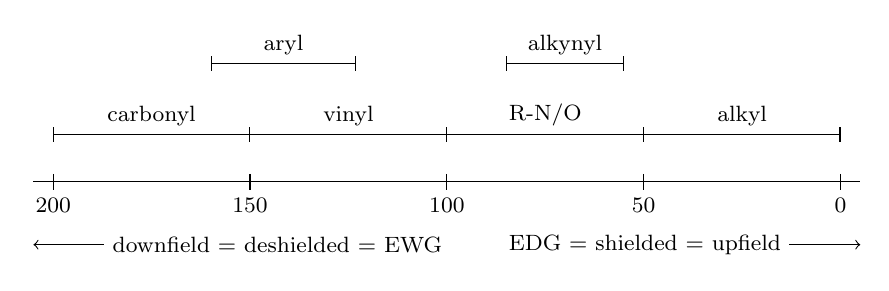
\begin{tikzpicture}[xscale=0.05]
            \footnotesize
            \draw (-205,0) -- (5,0);
            \foreach \x in {200,150,...,0} {
                \draw ({-\x},0.1) -- ++(0,-0.2) node[below]{$\x$};
            }
            \draw [<-] (-205,-0.8) -- ++(18,0) node[right]{downfield = deshielded = EWG};
            \draw [<-] (5,-0.8) -- ++(-18,0) node[left]{EDG = shielded = upfield};
    
            \draw [|-|] (-200,0.6) -- node[above]{carbonyl} (-150,0.6);
            \draw [-|]  (-150,0.6) -- node[above]{vinyl} (-100,0.6);
            \draw [-|]  (-100,0.6) -- node[above]{\ce{R-N/O}} (-50,0.6);
            \draw [-|]  (-50,0.6) -- node[above]{alkyl} (0,0.6);
            \draw [|-|] (-160,1.5) -- node[above]{aryl} (-123,1.5);
            \draw [|-|] (-85,1.5) -- node[above]{alkynyl} (-55,1.5);
        \end{tikzpicture}
        \caption{Chemical shifts of common carbon types.}
        \label{fig:chemShift13C}
    \end{figure}
    \begin{itemize}
        \item Note that we have a carbonyl region here that we did not have in Figure \ref{fig:chemShift1H}!
    \end{itemize}
    \item If \ce{{}^13C} NMR can be used for functional group identification, why would we ever want to use IR?
    \begin{itemize}
        \item There are some functional groups between which \ce{{}^13C} NMR can't distinguish.
        \begin{itemize}
            \item Example: \ce{{}^13C} NMR can't distinguish \ce{C=N} from \ce{C=O}, but IR can.
        \end{itemize}
        \item As a general rule, though, a chemist would collect data from both sources (as well as all the others) and make sure that the data is consistent.
        \begin{itemize}
            \item For example, if \ce{{}^13C} NMR suggests that a molecule has an alkynyl carbon but IR doesn't show a stretch at \SI{3300}{\per\centi\meter}, we might have a problem!
            \item One potential solution to this problem could be that we mistakenly identified a \ce{R-N/O} peak in the \ce{{}^13C} NMR spectrum as an alkynyl peak.
        \end{itemize}
    \end{itemize}
    \item We now return to \ce{{}^1H} NMR for some guidelines on interpreting these spectra.
    \begin{itemize}
        \item NMR can tell you how many distinct \ce{{}^1H}/\ce{{}^13C} groups you have, what kind of functional group they are, and how they're connected.
        \item Example step-by-step workflow for \ce{{}^1H} NMR.
        \begin{enumerate}
            \item Identify the number of unique peaks, and watch out for overlap!
            \item Note the chemical shifts and propose likely functional groups.
            \item Calculate or consider integrations.
            \item Observe the peak shape and start hypothesizing about connectivity.
            \item Calculate $J$ to confirm or support connectivity.
            \item Make sure that all the data is consistent.
        \end{enumerate}
    \end{itemize}
    \pagebreak
    \item Let's now look at an example of how we could identify a compound from its \ce{{}^1H} NMR spectrum using the above workflow.
    \item Example \ce{{}^1H} NMR spectrum: 4,4-Dimethylcyclohex-2-en-1-one (\,{\tiny\chemfig[baseline=1.1mm,atom sep=1em,bond offset=1pt,fixed length=false]{*6([:30]--(-[:20])(-[:-20])-=-(=O)-)}}\,).
    \begin{figure}[h!]
        \centering
        \setcharge{extra sep=8pt}
        \begin{tikzpicture}[text height=1.5ex,text depth=0.25ex,every node/.style=black]
            \small
            \draw (-12,4) -- node[rotate=90,above]{Intensity} (-12,0) -- node[below=4.7mm]{ppm} (0,0);
    
            \footnotesize
            \node [below=1mm] at (0,0) {0};
            \draw (-6,0.1) -- ++(0,-0.2) node[below]{6};
            \node [below=1mm] at (-12,0) {12};
    
            \draw [blx,semithick] (-12,0)
                -- (-6.73,0)
                to[out=0,in=180,out looseness=0.1,in looseness=0.06] (-6.68,0.5)
                to[out=0,in=180,out looseness=0.06,in looseness=0.1] (-6.63,0.15) node[above=10.5mm,align=center]{10.1\\d\\1H\\6.63}
                to[out=0,in=180,out looseness=0.1,in looseness=0.06] (-6.58,0.7)
                to[out=0,in=180,out looseness=0.06,in looseness=0.1] (-6.53,0)
                -- (-5.91,0)
                to[out=0,in=180,out looseness=0.1,in looseness=0.06] (-5.86,0.7)
                to[out=0,in=180,out looseness=0.06,in looseness=0.1] (-5.81,0.15) node[above=10.5mm,align=center]{10.1\\d\\1H\\5.81}
                to[out=0,in=180,out looseness=0.1,in looseness=0.06] (-5.76,0.5)
                to[out=0,in=180,out looseness=0.06,in looseness=0.1] (-5.71,0)
                -- (-2.52,0)
                to[out=0,in=180,out looseness=0.1,in looseness=0.06] (-2.49,0.6)
                to[out=0,in=180,out looseness=0.06,in looseness=0.1] (-2.46,0.15)
                to[out=0,in=180,out looseness=0.1,in looseness=0.06] (-2.43,1.2) node[above,align=center]{6.6\\t\\2H\\2.43}
                to[out=0,in=180,out looseness=0.06,in looseness=0.1] (-2.40,0.15)
                to[out=0,in=180,out looseness=0.1,in looseness=0.06] (-2.37,0.6)
                to[out=0,in=180,out looseness=0.06,in looseness=0.1] (-2.34,0)
                -- (-1.93,0)
                to[out=0,in=180,out looseness=0.1,in looseness=0.06] (-1.90,0.6)
                to[out=0,in=180,out looseness=0.06,in looseness=0.1] (-1.87,0.15)
                to[out=0,in=180,out looseness=0.1,in looseness=0.06] (-1.84,1.2) node[above,align=center]{6.6\\t\\2H\\1.84}
                to[out=0,in=180,out looseness=0.06,in looseness=0.1] (-1.81,0.15)
                to[out=0,in=180,out looseness=0.1,in looseness=0.06] (-1.78,0.6)
                to[out=0,in=180,out looseness=0.06,in looseness=0.1] (-1.75,0)
                -- (-1.21,0)
                to[out=0,in=180,out looseness=0.05,in looseness=0.03] (-1.14,2.7)
                to[out=0,in=180,out looseness=0.03,in looseness=0.05] (-1.07,0)
                -- (0,0)
            ;
            \node [above,align=center] at (-0.7,1.2) {s\\6H\\1.14};
            
            \node [circle,draw,inner sep=1pt,above=1mm] at (-6.63,2.7) {B};
            \node [circle,draw,inner sep=1pt,above=1mm] at (-5.81,2.7) {A};
            \node [circle,draw,inner sep=1pt,above=1mm] at (-2.43,2.7) {E};
            \node [circle,draw,inner sep=1pt,above=1mm] at (-1.84,2.7) {D};
            \node [circle,draw,inner sep=1pt,above=1mm] at (-1.14,2.7) {C};
    
            \node [above,align=right,font=\bfseries] at (-8.1,1.2) {$\bm{J}$ (Hz):\\Peak pattern:\\Integration:\\$\bm{\delta}$ (ppm):};
    
            \node (M) at (-10.5,2.5) {\chemfig[atom sep=1.4em]{*6(\charge{-150=\tikz{\node[circle,draw,inner sep=1pt]{D};}}{}
                -(-[:-70]\charge{-70=\tikz{\node[circle,draw,inner sep=1pt]{C};}}{})(-[:-110])
                -\charge{-30=\tikz{\node[circle,draw,inner sep=1pt]{B};}}{}
                =\charge{30=\tikz{\node[circle,draw,inner sep=1pt]{A};}}{}
                -(=O)
                -\charge{150=\tikz{\node[circle,draw,inner sep=1pt]{E};}}{}
                -)}
            };
        \end{tikzpicture}
        \caption{\ce{{}^1H} NMR spectrum of 4,4-dimethylcyclohex-2-en-1-one.}
        \label{fig:NMRdmceo}
    \end{figure}
    \begin{enumerate}
        \item There are 5 unique peaks.
        \begin{itemize}
            \item This means that there are 5 unique proton positions.
        \end{itemize}
        \item There are 2 peaks in the vinyl region,\footnote{Note that we include the peak at \SI{6.63}{\partspermillion} in the vinyl region even though it would normally fall in the aryl region (per Figure \ref{fig:chemShift1H}) due to the nearby carbonyl EWG.} and 3 peaks in the alkyl region.
        \item The ratio of integrations is $1:1:2:2:6$.
        \begin{itemize}
            \item The 6H integration must be 2 identical groups of 3 protons (i.e., methyl groups)!
            \item Similarly, if we saw 9H, it would probably be 3 identical methyl groups.
        \end{itemize}
        \item There are 2 roofing doublets, 2 triplets, and 1 singlet.
        \begin{itemize}
            \item The 2 roofing doublets correspond to the vinyl protons.
            \begin{itemize}
                \item This implies that our vinyl protons are adjacent to each other.
                \item Thus, part of our molecule looks like this: {\tiny\chemfig[baseline=-0.7mm,atom sep=1em,bond offset=1pt,fixed length=false]{(-[:120]H)(-[:-120]!{wave})=_(-[:60]H)(-[:-60]!{wave})}}
                \item Note that we will not know that the vinyl protons are \emph{cis} until Step 5; they could still be \emph{trans} or geminal until the coupling constant tells us otherwise.
            \end{itemize}
            \item The 2 triplets correspond to some of the alkyl protons.
            \begin{itemize}
                \item This splitting pattern implies the presence of two protons next to two protons.
                \item Thus, part of our molecule looks like this: {\tiny\chemfig[baseline=-0.7mm,atom sep=1em,bond offset=1pt,fixed length=false]{(-[:100]H)(-[:140]H)(-[:-120]!{wave})-(-[:80]H)(-[:40]H)(-[:-60]!{wave})}}
                \item Note that this splitting pattern analysis lines up with the integrations as well!
            \end{itemize}
            \item The 1 singlet corresponds to the remaining alkyl protons.
            \begin{itemize}
                \item Six chemically identical protons that are not split by anything implies geminal methyl groups on a tetrasubstituted carbon.
                \item Thus, part of our molecule looks like this: {\tiny\chemfig[baseline=-0.7mm,atom sep=1em,bond offset=1pt,fixed length=false]{(-[:-150]!{wave})(-[:-30]!{wave})(-[:70])(-[:110])}}
            \end{itemize}
        \end{itemize}
        \item The $J$'s agree with all the motifs we've proposed so far.
        \begin{itemize}
            \item The \SI{6.6}{\hertz} splitting of the triplets doesn't get us much new information.
            \item However, per Figure \ref{fig:couplingVinyl} and the associated discussion, a coupling constant of \SI{10.1}{\hertz} for the vinyl protons confirms that they are in a \emph{cis} orientation, as drawn above.
        \end{itemize}
        \item All of the data is, indeed, consistent with the proposed molecule's structure.
    \end{enumerate}
\end{itemize}



\section{Structure Determination - 1}
\begin{itemize}
    \item \marginnote{9/16:}Lecture 5 recap: A review of the suggested \ce{{}^1H} NMR interpretation workflow.
    \begin{enumerate}
        \item Identify unique peaks: Tells you if the molecule has symmetry.
        \begin{itemize}
            \item Example: 6 protons but 4 peaks.
        \end{itemize}
        \item Chemical shifts: Tells you which functional groups may be present.
        \item Integrations: Tells you how many protons there are at each position in the molecule.
        \item Peak shape: Tells you which protons neighbor which other protons.
        \item $J$ values: Tells you which protons \emph{really} neighbor which other protons.
        \begin{itemize}
            \item Example: If two peaks share a coupling constant, they correspond to neighboring protons.
        \end{itemize}
        \item Sanity check: Ensures that all your hypotheses derived from the previous steps are consistent.
    \end{enumerate}
    \item Today: Structure determination.
    \begin{itemize}
        \item Reading: \textcite{bib:Clayden}, Chapter 18.
        \item This reading covers several examples of when NMR is really useful. In some of these examples, NMR is the technique \emph{needed} to solve a problem.
        \item There's a good bit of stuff that's beyond the scope of the class, but it's really short (only 20 pages) and will be very helpful for you, so please read it!!
    \end{itemize}
    \item Lecture outline.
    \begin{itemize}
        \item Overview and recap of the 5 structure determination methods we've discussed to date.
        \item Key signals across the 5 methods.
        \item Examples of when certain techniques are more useful.
    \end{itemize}
    \item Methods overview.
    \begin{itemize}
        \item EA: Get the empirical formula.
        \item MS: Get the molecular formula, isotope identities, stable fragments, and fragmentation patterns.
        \begin{itemize}
            \item Fragmentation patterns tell us a lot about connectivity.
        \end{itemize}
        \item IR: Get key functional groups.
        \item \ce{{}^13C} NMR: Get the number of unique carbons, key functional groups.
        \begin{itemize}
            \item The number of unique carbons gives info on molecular symmetry.
        \end{itemize}
        \item \ce{{}^1H} NMR: Get the number of unique protons, key functional groups, and data about connectivity.
        \begin{itemize}
            \item The relevant connectivity data here comes from $J$ values.
        \end{itemize}
    \end{itemize}
    \item Why do we need multiple analytical techniques for key functional groups?
    \begin{itemize}
        \item A single spectrum rarely contains the full picture. Rather, each technique gives a hint, and we --- as chemists --- are like detectives following the different lines of inquiry.
        \item Different spectra can help in a \emph{confirmational} manner or an \emph{orthogonal} manner.
        \begin{itemize}
            \item Confirmational: Both IR and \ce{{}^13C} NMR show a ketone, so I'm pretty sure there's a ketone!
            \item Orthogonal: Here's a new piece of information that none of the other techniques have given me yet.
        \end{itemize}
        \item Critical point: The final proposed molecular structure must be consistent with \emph{all} data.
        \begin{itemize}
            \item If you're matching the IR and the \ce{{}^1H} NMR but not the \ce{{}^13C} NMR, it can't be right!
        \end{itemize}
    \end{itemize}
    \item We now look into some common signals and what they tell us.
    \item Shortcuts: "Give away" signals.
    \begin{itemize}
        \item Bromine and chlorine in MS.
        \item \ce{C=O} in IR and \ce{{}^13C} NMR.
        \item OH stretch in IR and the (typically) broad peak in \ce{{}^1H} NMR.
        \item \ce{CH3} peaks in \ce{{}^1H} NMR (i.e., upfield peaks that integrate to 3H) and MS (i.e., $\cnc{M$-15$}^+$ peaks).
        \item Aldehyde protons in the $\SIrange{10}{11}{\partspermillion}$ region of \ce{{}^1H} NMR.
        \item Roofing doublets in the aromatic region of \ce{{}^1H} NMR.
        \begin{itemize}
            \item Tends to indicate a \emph{para}-substituted benzene ring with different substituents on both sides.
        \end{itemize}
        \item And more! Practice, and notice trends!!
    \end{itemize}
    \item Let's do some practice now on some particularly hard examples.
    \item Consider the following isomers.
    \begin{figure}[h!]
        \centering
        \footnotesize
        \begin{subfigure}[b]{0.2\linewidth}
            \centering
            \chemfig{-[:30](=[2]O)-[:-30](<[6]OH)-[:30](<[2]OH)-[:-30]}
            \caption{Original structure.}
            \label{fig:isomerIdenta}
        \end{subfigure}
        \begin{subfigure}[b]{0.18\linewidth}
            \centering
            \chemfig{-[:30](=[2]O)-[:-30](<:[6]OH)-[:30](<:[2]OH)-[:-30]}
            \caption{Enantiomer.}
            \label{fig:isomerIdentb}
        \end{subfigure}
        \begin{subfigure}[b]{0.18\linewidth}
            \centering
            \chemfig{-[:30](=[2]O)-[:-30](<[6]OH)-[:30](<:[2]OH)-[:-30]}
            \caption{Diastereomer.}
            \label{fig:isomerIdentc}
        \end{subfigure}
        \begin{subfigure}[b]{0.23\linewidth}
            \centering
            \chemfig{-[:30](<[2]OH)-[:-30](=[6]O)-[:30](<[2]OH)-[:-30]}
            \caption{Constitutional isomer.}
            \label{fig:isomerIdentd}
        \end{subfigure}
        \caption{Isomer identification with structure determination.}
        \label{fig:isomerIdent}
    \end{figure}
    \item If we try to distinguish the original structure (Figure \ref{fig:isomerIdenta}) from any of the others using the structure determination techniques, we'll find that the results are\dots
    \begin{table}[h!]
        \centering
        \small
        \renewcommand{\arraystretch}{1.2}
        \begin{tabular}{rccc}
             & \textbf{Enantiomer} & \textbf{Diastereomer} & \textbf{Constitutional isomer}\\
            \textbf{EA:} & identical & identical & identical\\
            \textbf{MS:} & identical & similar & different\\
            \textbf{IR:} & identical & similar & different\\
            \textbf{\ce{{}^13C} NMR:} & identical & different & different\\
            \textbf{\ce{{}^1H} NMR:} & identical & different & different\\
        \end{tabular}
        \caption{Isomer identification with structure determination.}
        \label{tab:isomerIdent}
    \end{table}
    \begin{itemize}
        \item Distinguishing the enantiomer.
        \begin{itemize}
            \item In order to distinguish chiral materials, you have to have a chiral technique.
            \item Specificaly, you would need a chiral light source to distinguish chiral molecules.
            \begin{itemize}
                \item We'll talk on Wednesday about IR with plane polarized light (Circular Dichroism), which would work, but we don't have that technique yet.
            \end{itemize}
            \item The only time the enantiomers could be distinguished using any of the techniques we've learned so far is with a weird edge case like a chiral solvent.
        \end{itemize}
        \item Distinguishing the diastereomer.
        \begin{itemize}
            \item Diastereomers can look different on MS and IR, but it's subtle. This is why we say \emph{similar}.
            \item With \ce{{}^13C} NMR, the peaks are technically different, but practically similar.
            \item With \ce{{}^1H} NMR, the Karplus equation makes certain $J$ values larger or smaller depending on the diastereomer.
            \begin{itemize}
                \item This can help us differentiate gauche, syn, and anti conformations.
            \end{itemize}
            \item Chapter 13 of \textcite{bib:Clayden} has more on distinguishing diastereomers; read it!!
        \end{itemize}
        \item Distinguishing the constitutional isomer.
        \begin{itemize}
            \item This molecule has a plane of symmetry, and thus only 3 unique carbons; this makes this molecule much easier to pick out using the techniques we know (e.g., \ce{{}^13C} NMR).
        \end{itemize}
    \end{itemize}
    \item Example: Determine the structure of the molecule described by the following data.
    \begin{itemize}
        \item \ce{{}^13C} NMR: $\delta$ 171.4, 60.5, 21.0, 14.2.
        \begin{itemize}
            \item Per Figure \ref{fig:chemShift13C}, these peaks respectively correspond to a carbonyl, \ce{C-X},\footnote{Recall that "\ce{X}" is a placeholder for some as-of-yet-undetermined electronegative heteroatom, such as oxygen, nitrogen, or a halogen.} and two alkyl carbons.
        \end{itemize}
        \item \ce{{}^1H} NMR: $\delta$ 4.12 (q, 2H), 2.05 (s, 3H), 1.26 (t, 3H).
        \begin{itemize}
            \item The middle peak corresponds to a methyl group: {\tiny\chemfig[baseline=0mm,atom sep=1em,bond offset=1pt,fixed length=false]{CH_3-[4]!{wave}}}
            \item The left peak corresponds to a \ce{C-X}, with 2H bonded to the C and 3H adjacent (it's split into a quartet): {\tiny\chemfig[baseline=0.5mm,atom sep=1em,bond offset=1pt,fixed length=false]{X-[:30](-[:70]H)(-[:110]H)-[:-30](-[:30]H)(-[:-30]H)(-[6]H)}}
            \item The right peak probably corresponds to the adjacent 3H introduced above. This is because we'd predict that the adjacent 3H introduced above would be an alkyl 3H that gets split into a triplet, just like the right peak.
        \end{itemize}
        \item After this initial analysis, redraw the biggest fragment and start combining fragments.
        \begin{itemize}
            \item We could try bonding the ethyl-X group into the other methyl group (\,{\tiny\chemfig[baseline=-1.3mm,atom sep=1em,bond offset=1pt,fixed length=false]{H_3C-[:-30,1.4]X-[:30]-[:-30]}}\,), but this would leave no space for the carbonyl.
            \item Thus, we can bond into the carbonyl and then the methyl group: {\tiny\chemfig[baseline=1mm,atom sep=1em,bond offset=1pt,fixed length=false]{H_3C-[:30](=[2]O)-[:-30]X-[:30]-[:-30]}}
        \end{itemize}
        \item The last thing we have to determine now is the identity of the heteroatom \ce{X}.
        \begin{itemize}
            \item If \ce{X} is a halogen, then the above structure implies that it's divalent. Since halogens don't like to form more than 1 bond, \ce{X} is probably not a halogen.
            \item If $\ce{X}=\ce{NH}$, then this proton would have a \ce{{}^1H} NMR signal as well and should have shown up in the data.
            \begin{itemize}
                \item The proton could be \ce{{}^1H} NMR silent due to exchange, but we should probably \textbf{Occam's razor} that possibility out.
            \end{itemize}
            \item If $\ce{X}=\ce{O}$, then there would be no extra \ce{{}^1H} NMR signals: {\tiny\chemfig[baseline=1mm,atom sep=1em,bond offset=1pt,fixed length=false]{H_3C-[:30](=[2]O)-[:-30]O-[:30]-[:-30]}}
            \begin{itemize}
                \item This structure is consistent with all the data we have, so we can be confident that we have determined the structure.
            \end{itemize}
        \end{itemize}
        \item This molecule is called ethyl acetate, and every organic chemist knows it because it's a common laboratory solvent and traces of it often appear in our NMR experiments.
    \end{itemize}
    \item \textbf{Occam's razor}: The simplest explanation is usually the best explanation.
    \item Maxim: Occam's razor is king with structure determination.
    \item Example: Describe how you would use the key signal(s) in the structure determination data of the following two compounds to tell them apart.
    \begin{figure}[h!]
        \centering
        \footnotesize
        \begin{subfigure}[b]{0.3\linewidth}
            \centering
            \chemfig{-[:30]*6(=-=(-(=[2]O)-[:-30]Cl)-=-)}
            \caption{\emph{p}-Toluoyl chloride.}
            \label{fig:compoundDiffa}
        \end{subfigure}
        \begin{subfigure}[b]{0.3\linewidth}
            \centering
            \chemfig{*6(=-=(--[:-30](=[6]O)-[:30]Cl)-=-)}
            \caption{Phenylacetyl chloride.}
            \label{fig:compoundDiffb}
        \end{subfigure}
        \caption{Two compounds to differentiate using structure determination.}
        \label{fig:compoundDiff}
    \end{figure}
    \begin{itemize}
        \item EA key signals? No.
        \begin{itemize}
            \item The molecules have identical empirical formulas.
        \end{itemize}
        \item MS key signals? Tough.
        \begin{itemize}
            \item We'd get $\alpha$-cleavage with both ketones, leading to similar fragments.
        \end{itemize}
        \item IR key signals? Tough.
        \begin{itemize}
            \item The \ce{C=O} stretch would be the main IR-active signal, and both carbonyls are fairly similar.
        \end{itemize}
        \item \ce{{}^13C} NMR key signals? Tough.
        \begin{itemize}
            \item The molecules have roughly the same symmetry (8 carbons, 6 unique ones).
        \end{itemize}
        \item \ce{{}^1H} NMR key signals? Yes: Multiple key signals!
        \begin{itemize}
            \item Let's start in the alkyl region.
            \begin{itemize}
                \item Both molecules would have one alkyl peak: Figure \ref{fig:compoundDiffa} has a methyl group at the bottom-left of the aromatic ring, and Figure \ref{fig:compoundDiffb} has a methylene group connecting the aromatic ring to the acid chloride.
                \item The methyl group will appear as a 3H singlet between $\SIrange{1}{2}{\partspermillion}$.
                \item The methylene group will appear as a 2H singlet between $\SIrange{2}{4}{\partspermillion}$ (it is more downfield due to the nearby EWGs).
            \end{itemize}
            \item The peaks in the aryl region will also be different.
            \begin{itemize}
                \item For Figure \ref{fig:compoundDiffa}, the protons will split into two roofing doublets, both of which integrate to 2H.
                \item For Figure \ref{fig:compoundDiffb}, the protons will split into a 2H doublet, a 2H doublet of doublets, and a 1H triplet.
                \item However, note that for Figure \ref{fig:compoundDiffb}, the actual aromatic peaks of this molecule show up as what we call a "multiplet (m)," meaning that it is a messy mound of peaks that we can't assign a clean pattern to because they overlap too much. You can still integrate the multiplet and see that it contains 5H, and that's how you could differentiate this molecule from the other in practice.
            \end{itemize}
        \end{itemize}
    \end{itemize}
\end{itemize}



\section{Structure Determination - 2}
\begin{itemize}
    \item \marginnote{9/18:}Lecture 6 recap: The journey from having a liquid to having the liquid's molecular structure.
    \begin{enumerate}
        \item EA: Get the empirical formula.
        \item MS (parent peak): Transform the empirical formula to the molecular formula.
        \item IR: Get key functional groups.
        \item \ce{{}^13C} NMR: Get the number of unique carbons, and confirm key functional groups.
        \item \ce{{}^1H} NMR: Get data about connecting fragments, and confirm key functional groups.
        \item MS (fragments): Confirm connectivity data.
        \item Double check: Does the proposed structure align with \emph{all} information?
    \end{enumerate}
    \item Autumn-themed aside: Eugenol (cloves) and cinnamaldehyde (cinnamon) make up pumpkin spice!
    \item Today: More structure determination.
    \item Lecture outline.
    \begin{itemize}
        \item Ring currents.
        \item X-ray crystallography.
        \item Circular dichroism.
        \item Structure determination practice.
    \end{itemize}
    \item Note that X-ray and CD won't be on Exam 1, but they will be useful for any lab work we do.
    \pagebreak
    \item Ring currents and related effects.
    \begin{figure}[h!]
        \centering
        \vspace{4em}
        \footnotesize
        \begin{subfigure}[b]{0.28\linewidth}
            \centering
            \chemfig{@{a}-[:20]@{b}-[:-3]H}
            \chemmove{
                \filldraw [-,thick,draw=orx,fill=ory] ($(a)+(0.0018,0.1)$) to[bend right=110,looseness=600] ($(a)+(-0.0018,0.1)$);
                \filldraw [-,thick,draw=orx,fill=white] ($(a)+(-0.0018,-0.1)$) to[bend right=110,looseness=600] ($(a)+(0.0018,-0.1)$);
                \filldraw [-,thick,draw=orx,fill=ory] ($(b)+(0.0018,0.1)$) to[bend right=110,looseness=600] ($(b)+(-0.0018,0.1)$);
                \filldraw [-,thick,draw=orx,fill=white] ($(b)+(-0.0018,-0.1)$) to[bend right=110,looseness=600] ($(b)+(0.0018,-0.1)$);
            }
            \vspace{2.3em}
            \caption{Vinyl deshielding.}
            \label{fig:ringCurrenta}
        \end{subfigure}
        \begin{subfigure}[b]{0.4\linewidth}
            \centering
            \chemfig[atom sep=3em]{@{a}-[,1.3]@{b}-[:30,1]@{c}-[:130,0.8]@{d}-[4,1.3]@{e}-[:-150,1]@{f}-[:-50,0.8]}
            \chemmove{
                \filldraw [-,thick,draw=orx,fill=white] ($(a)+(0.0018,0.1)$) to[bend right=110,looseness=600] ($(a)+(-0.0018,0.1)$);
                \filldraw [-,thick,draw=orx,fill=ory] ($(a)+(-0.0018,-0.1)$) to[bend right=110,looseness=600] ($(a)+(0.0018,-0.1)$);
                \filldraw [-,thick,draw=orx,fill=white] ($(b)+(0.0018,0.1)$) to[bend right=110,looseness=600] ($(b)+(-0.0018,0.1)$);
                \filldraw [-,thick,draw=orx,fill=ory] ($(b)+(-0.0018,-0.1)$) to[bend right=110,looseness=600] ($(b)+(0.0018,-0.1)$);
                \filldraw [-,thick,draw=orx,fill=white] ($(c)+(0.0018,0.1)$) to[bend right=110,looseness=600] ($(c)+(-0.0018,0.1)$);
                \filldraw [-,thick,draw=orx,fill=ory] ($(c)+(-0.0018,-0.1)$) to[bend right=110,looseness=600] ($(c)+(0.0018,-0.1)$);
                \filldraw [-,thick,draw=orx,fill=white] ($(d)+(0.0018,0.1)$) to[bend right=110,looseness=600] ($(d)+(-0.0018,0.1)$);
                \filldraw [-,thick,draw=orx,fill=ory] ($(d)+(-0.0018,-0.1)$) to[bend right=110,looseness=600] ($(d)+(0.0018,-0.1)$);
                \filldraw [-,thick,draw=orx,fill=white] ($(e)+(0.0018,0.1)$) to[bend right=110,looseness=600] ($(e)+(-0.0018,0.1)$);
                \filldraw [-,thick,draw=orx,fill=ory] ($(e)+(-0.0018,-0.1)$) to[bend right=110,looseness=600] ($(e)+(0.0018,-0.1)$);
                \filldraw [-,thick,draw=orx,fill=white] ($(f)+(0.0018,0.1)$) to[bend right=110,looseness=600] ($(f)+(-0.0018,0.1)$);
                \filldraw [-,thick,draw=orx,fill=ory] ($(f)+(-0.0018,-0.1)$) to[bend right=110,looseness=600] ($(f)+(0.0018,-0.1)$);
            }
            \begin{tikzpicture}[remember picture,overlay]
                \draw [->] (0.6,-0.5) -- ++(0,2);
                \draw [->] (1,-0.5) -- ++(0,2);
                \draw [->] (0.8,-0.5) -- node[align=center,fill=white]{external\\magnetic\\field} ++(0,2);
    
                \draw [gax,thick,-latex] (-1.45,2.2) arc[start angle=90,end angle=-250,x radius=1cm,y radius=0.4cm];
                \draw [gax,thick,-latex] (-1.45,-0.8) arc[start angle=90,end angle=-250,x radius=1cm,y radius=0.4cm];
                \node [align=center] at (-1.45,-1.22) {$\pi$-electrons\\circling};
            \end{tikzpicture}
            \vspace{5.1em}
            \caption{Ring current induced.}
            \label{fig:ringCurrentb}
        \end{subfigure}
        \begin{subfigure}[b]{0.28\linewidth}
            \centering
            \chemfig[atom sep=3em]{@{a}-[,1.3]@{b}-[:30,1]@{c}(-[,0.6]H)-[:130,0.8]@{d}-[4,1.3]@{e}-[:-150,1]@{f}(-[6,0.6,,,opacity=0]\phantom{H})-[:-50,0.8]}
            \chemmove{
                \filldraw [-,thick,draw=orx,fill=white] ($(a)+(0.0018,0.1)$) to[bend right=110,looseness=600] ($(a)+(-0.0018,0.1)$);
                \filldraw [-,thick,draw=orx,fill=ory] ($(a)+(-0.0018,-0.1)$) to[bend right=110,looseness=600] ($(a)+(0.0018,-0.1)$);
                \filldraw [-,thick,draw=orx,fill=white] ($(b)+(0.0018,0.1)$) to[bend right=110,looseness=600] ($(b)+(-0.0018,0.1)$);
                \filldraw [-,thick,draw=orx,fill=ory] ($(b)+(-0.0018,-0.1)$) to[bend right=110,looseness=600] ($(b)+(0.0018,-0.1)$);
                \filldraw [-,thick,draw=orx,fill=white] ($(c)+(0.0018,0.1)$) to[bend right=110,looseness=600] ($(c)+(-0.0018,0.1)$);
                \filldraw [-,thick,draw=orx,fill=ory] ($(c)+(-0.0018,-0.1)$) to[bend right=110,looseness=600] ($(c)+(0.0018,-0.1)$);
                \filldraw [-,thick,draw=orx,fill=white] ($(d)+(0.0018,0.1)$) to[bend right=110,looseness=600] ($(d)+(-0.0018,0.1)$);
                \filldraw [-,thick,draw=orx,fill=ory] ($(d)+(-0.0018,-0.1)$) to[bend right=110,looseness=600] ($(d)+(0.0018,-0.1)$);
                \filldraw [-,thick,draw=orx,fill=white] ($(e)+(0.0018,0.1)$) to[bend right=110,looseness=600] ($(e)+(-0.0018,0.1)$);
                \filldraw [-,thick,draw=orx,fill=ory] ($(e)+(-0.0018,-0.1)$) to[bend right=110,looseness=600] ($(e)+(0.0018,-0.1)$);
                \filldraw [-,thick,draw=orx,fill=white] ($(f)+(0.0018,0.1)$) to[bend right=110,looseness=600] ($(f)+(-0.0018,0.1)$);
                \filldraw [-,thick,draw=orx,fill=ory] ($(f)+(-0.0018,-0.1)$) to[bend right=110,looseness=600] ($(f)+(0.0018,-0.1)$);
            }
            \begin{tikzpicture}[remember picture,overlay]
                \draw [gax,thick,-latex] (-1.9,-0.2) arc[start angle=-150,end angle=150,x radius=0.8cm,y radius=1.3cm];
                \draw [gax,thick,-latex] (-2.4,-0.2) arc[start angle=-30,end angle=-330,x radius=0.8cm,y radius=1.3cm];
            \end{tikzpicture}
            \vspace{2.3em}
            \caption{New magnetic field.}
            \label{fig:ringCurrentc}
        \end{subfigure}\\[2em]
        \begin{subfigure}[b]{0.38\linewidth}
            \centering
            \begin{tikzpicture}
                \node (M) {\chemfig{*6(--=---)}};
                \node at (1.2,-0.4) {\SI{5.7}{\partspermillion}}
                    edge [->,bend right=20] (M.20) 
                ;
                \path (-1.8,0) -- (1.8,0);
            \end{tikzpicture}
            \caption{Cyclohexene.}
            \label{fig:ringCurrentd}
        \end{subfigure}
        \begin{subfigure}[b]{0.2\linewidth}
            \centering
            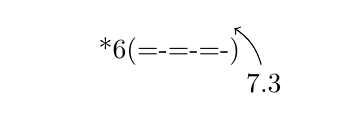
\begin{tikzpicture}
                \node (M) {\chemfig{*6(=-=-=-)}};
                \node at (1.2,-0.4) {\SI{7.3}{\partspermillion}}
                    edge [->,bend right=20] (M.20) 
                ;
                \path (-1.8,0) -- (1.8,0);
            \end{tikzpicture}
            \caption{Benzene.}
            \label{fig:ringCurrente}
        \end{subfigure}
        \begin{subfigure}[b]{0.38\linewidth}
            \centering
            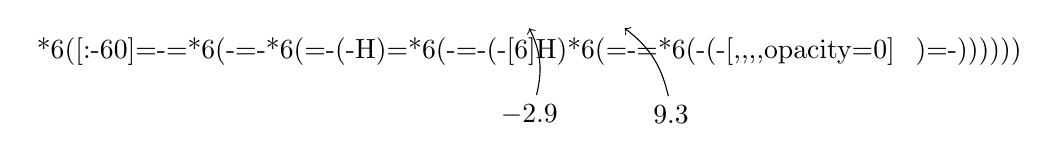
\begin{tikzpicture}
                \node (M) {\chemfig{*6([:-60]=-=*6(-=-*6(=-(-H)=*6(-=-(-[6]H)*6(=-=*6(-(-[,,,,opacity=0]\phantom{H})=-))))))}};
                \node at (1.8,-0.8) {\SI{9.3}{\partspermillion}}
                    edge [->,bend right=20] ([xshift=-2mm]M.12) 
                ;
                \node at (0,-0.8) {$-\SI{2.9}{\partspermillion}$}
                    edge [->,bend right=20] (0,0.3) 
                ;
                \path (-2.5,0) -- (2.5,0);
            \end{tikzpicture}
            \caption{[18]annulene.}
            \label{fig:ringCurrentf}
        \end{subfigure}
        \caption{Ring currents and related effects.}
        \label{fig:ringCurrent}
    \end{figure}
    \begin{itemize}
        \item Protons next to $\pi$-systems are deshielded.
        \begin{itemize}
            \item Example: Cyclohexene's vinyl protons are downfield at \SI{5.7}{\partspermillion} (see Figure \ref{fig:ringCurrentd}).
            \item Alkene protons are deshielded because they lie in the nodal plane of the $\pi$-system, coplanar with the so-called "$\sigma$-bond network." This means that much of the electron density is above or below these protons in the $p$-lobes. Thus, the protons have less electron density near them, which we observe as deshielding (see Figure \ref{fig:ringCurrenta}).
        \end{itemize}
        \item While cyclohexene's vinyl protons are certainly deshielded compared to normal alkyl protons, benzene's six protons are even more deshielded, lying at \SI{7.3}{\partspermillion}.
        \item What makes aromatic protons so much more deshielded?
        \begin{itemize}
            \item When benzene is placed in an external magnetic field, it orients itself perpendicular to the magnetic field because the $p$-orbitals all want to align with the magnetic field (see Figure \ref{fig:ringCurrentb}).
            \begin{itemize}
                \item Once benzene is oriented, the magnetic field causes the $\pi$-electrons to circle around the ring system.
            \end{itemize}
            \item These rotating electrons create a new magnetic field (see Figure \ref{fig:ringCurrentc}).
            \begin{itemize}
                \item This small, local magnetic field reinforces the external magnetic field, deshielding the external protons.
            \end{itemize}
            \item Prediction: In an aromatic ring big enough to have \emph{internal} protons (see Figure \ref{fig:ringCurrentf}), such protons will be extra shielded.
            \begin{itemize}
                \item Indeed, this prediction is experimentally confirmed: The internal protons of [18]annulene have a whopping $-\SI{2.9}{\partspermillion}$ chemical shift.
            \end{itemize}
            \item More $\pi$-electrons increases the ring current and ups the external protons' chemical shift, too.
            \item There's much more physics here, if you're curious!! But it's beyond the scope of the course.
        \end{itemize}
        \item Ring currents of aromatic compounds have tons of applications to organic semiconductors, etc.
    \end{itemize}
    \item X-ray crystallography.
    \begin{figure}[H]
        \centering
        \footnotesize
        \begin{subfigure}[b]{0.3\linewidth}
            \centering
            \chemfig[fixed length=false]{-[:30]-[:-30](=[6]O)-[:30](-[2]Br)-[:-30]}
            \caption{2-bromopentan-3-one.}
            \label{fig:xRayCrystala}
        \end{subfigure}
        \begin{subfigure}[b]{0.3\linewidth}
            \centering
            \chemfig[fixed length=false,bond offset=0pt]{@{5}-[:30]@{4}-[:-30]@{3}(-[6,0.8]@{3a}\phantom{O})-[:30]@{2}(-[2,1.2]@{2a}\phantom{Br})-[:-30]@{1}}
            \chemmove{
                \filldraw [fill=white] (5) circle (1.2mm);
                \filldraw [fill=white] (4) circle (1.2mm);
                \filldraw [fill=white] (3) circle (1.2mm);
                \filldraw [fill=white] (2) circle (1.2mm);
                \filldraw [fill=white] (1) circle (1.2mm);
                % 
                \filldraw [fill=white] (3a) circle (1.6mm);
                \filldraw [fill=white] (2a) circle (3.4mm);
            }
            \caption{X-ray structure.}
            \label{fig:xRayCrystalb}
        \end{subfigure}
        \caption{X-ray crystallography.}
        \label{fig:xRayCrystal}
    \end{figure}
    \begin{itemize}
        \item To begin, you grow a \textbf{crystal} of your sample.
        \item We then shoot X-rays at the crystal.
        \begin{itemize}
            \item We choose \emph{X-rays}, in particular, from among all types of light because their wavelength is approximately \SI{1}{\angstrom}. This is on the same order  of magnitudeas most bond lengths, so we get nice interactions, described as follows.
        \end{itemize}
        \item Specifically, these X-rays \textbf{diffract} when they hit a nucleus, and then we measure the location to which they bounce back.
        \begin{itemize}
            \item X-rays don't interact with electrons so much; they more interact with hard, heavy, localized nuclei.
            \item We have detectors all around the sample, and this allows us to back-calculate the positions of the nuclei.
        \end{itemize}
        \item The result of this data collection is that we know the exact position of every nucleus in every atom of our crystal.
        \begin{itemize}
            \item Once we have these positions, we can connect the dots to identify bonds.
            \item So to clarify, X-rays do not "see" the bonds directly, but if two nuclei are \SI{1.4}{\angstrom} apart (for example), then we can reasonably assume that \SI{1.4}{\angstrom} is the bond length.
        \end{itemize}
        \item Result: We get a 3D structure of our molecule with exact connectivity.
        \item Example: How a molecule looks to X-ray crystallography (see Figure \ref{fig:xRayCrystal}).
        \begin{itemize}
            \item To reiterate, every atom looks like a ball with size proportional to how much it weighs.
            \begin{itemize}
                \item For example, bromine is really heavy, so it shows up as a really big ball.
            \end{itemize}
            \item Once we have the atoms' positions, we --- as analysts --- draw in the bonds ourselves.
            \begin{itemize}
                \item For example, we know that \ce{C=O} bonds (as double bonds) tend to be shorter than single bonds, so it should not be surprising that the oxygen and C3 atoms appear closer together than any others.
            \end{itemize}
        \end{itemize}
    \end{itemize}
    \item \textbf{Crystal}: A regular lattice of repeating \textbf{unit cells}.
    \item \textbf{Unit cell}: The simplest thing that repeats.
    \item Pros and cons of X-ray diffraction.
    \begin{itemize}
        \item Pros:
        \begin{itemize}
            \item It's super awesome: gives you an exact 3D picture of the molecule.
            \item Can show you atoms that don't have NMR signals (like bromine).
            \item Often considered the "smoking gun" in structure determination. That is to say, X-ray crystallography is the spectroscopic technique that produces results you can't really argue with.
        \end{itemize}
        \item Cons.
        \begin{itemize}
            \item It's expensive ($\sim$\$1000/run).
            \item You can't just push a button, like you can with NMR.
            \begin{itemize}
                \item Rather, you need a technician to set the sample and an analyst to interpret the data (there's an art to it).
            \end{itemize}
            \item It's hard to grow crystals of certain compounds.
            \item You can't see the hydrogens because they're very small, but that's usually not an issue because we can infer where they are from all the other data.
            \item This \emph{crystal} structure naturally represents the molecule is the solid phase.
            \begin{itemize}
                \item This means that we don't get much information on the molecule's dynamics in solution (for example).
            \end{itemize}
        \end{itemize}
    \end{itemize}
    \item Circular dichroism (CD).
    \begin{figure}[h!]
        \centering
        \footnotesize
        \begin{subfigure}[b]{0.47\linewidth}
            \centering
            \begin{tikzpicture}[every node/.style=black]
                \node {\chemfig{Me-[:30](<[2]Br)-[:-30]Et}};
        
                \draw [rex,semithick,decorate,decoration={coil,aspect=0.9,amplitude=2mm},-latex] (-3.2,0) -- node[below=2mm]{L} (-1,0);
                \draw [rex,semithick,decorate,decoration={coil,aspect=0.9,amplitude=2mm},-latex] (1,0) -- node[below=2mm]{L} (3.2,0);
            \end{tikzpicture}
            \caption{Absorption of L light.}
            \label{fig:schematicCDa}
        \end{subfigure}
        \begin{subfigure}[b]{0.47\linewidth}
            \centering
            \begin{tikzpicture}[every node/.style=black]
                \node {\chemfig{Me-[:30](<[2]Br)-[:-30]Et}};
        
                \draw [rex,semithick,decorate,decoration={coil,aspect=0.9,amplitude=1mm,segment length=5pt,pre length=7pt},latex-,rotate=180] (-2.4,0) -- node[below=2mm]{R} (-1,0);
                \draw [rex,semithick,decorate,decoration={coil,aspect=0.9,amplitude=2mm,pre length=7pt},latex-,rotate=180] (1,0) -- node[below=2mm]{R} (3.2,0);
            \end{tikzpicture}
            \caption{Absorption of R light.}
            \label{fig:schematicCDb}
        \end{subfigure}
        \caption{Circular dichroism spectrophotometer schematic.}
        \label{fig:schematicCD}
    \end{figure}
    \begin{itemize}
        \item CD can be used to differentiate enantiomers!
        \item Uses circularly polarized light, that is, light that rotates either left or right.
        \begin{itemize}
            \item Circularly polarized light is created with a \textbf{polarimeter}.
        \end{itemize}
        \item Once the light is created, you shoot it at your sample and see what gets absorbed.
        \begin{itemize}
            \item Some molecules --- e.g., (\emph{R})-2-bromobutane --- will not absorb the L light, but will absorb some of the R light.
            \item Note the similarities between Figure \ref{fig:schematicCD} and Figure \ref{fig:schematicIR}.
        \end{itemize}
        \item One enantiomer will absorb one handedness of light, and the other enantiomer will absorb the other handedness of light.
        \begin{itemize}
            \item I.e., one enantiomer absorbs L and the other enantiomer absorbs R.
            \item You don't know which enantiomer will absorb which light before you test it!
            \item Implication: It's not always that (\emph{R})-enantiomers absorb R-light. It's just that one will absorb one, and the other will absorb the other.
        \end{itemize}
        \item CD allows us to calculate the \textbf{specific rotation} of a molecule.
        \item Example measurement of $[\alpha]$: 2-bromobutane.
        \begin{itemize}
            \item The (\emph{R})-enantomier has $[\alpha]=\ang{-23.1}$,\footnote{Verbally, we say, "the R enantiomer rotates plane-polarized light by 23 degrees in the negative direction."} and the (\emph{S})-enantiomer has $[\alpha]=+\ang{23.1}$.
            \item For a racemic mixture, $[\alpha]=\ang{0}$.
            \item If you have an $80:20$ mixture $R:S$, then this mixture has 60\% ee. This is because in an $80:20$ ratio, the 20\% of the sample that's (\emph{S}) cancels out 20\% of the sample that's (\emph{R}). Thus, the ee is $80\%-20\%=60\%$. It follows that $[\alpha]=-\ang{13.9}$.
        \end{itemize}
        \item It follows from the last line above that CD can be used to measure the ee of your system!
    \end{itemize}
    \item \textbf{Specific rotation} (of a molecule): A measure of the degree to which a molecule at temperature $T$ rotates plane-polarized light of wavelength $\lambda$. \emph{Denoted by} $\bm{[\alpha]_\lambda^T}$.
    \begin{itemize}
        \item We calculate this using both the sign ($+/-$) and the amplitude of the light after passing through the sample.
        \item The typical temperature is \SI{25}{\celsius}, and the typical wavelength is \SI{589}{\nano\meter}.
    \end{itemize}
    \item How do you obtain a pure sample of your enantiomer for an initial CD experiment, i.e., how do you know what 100\% ee looks like?
    \begin{itemize}
        \item There are methods that can purify enantiomers, like chiral column chromatography.
        \item Thus, even if your reaction doesn't yield 100\% ee, you can separate the products into two samples that are 100\% ee and 0\% ee, and analyze those first.
    \end{itemize}
    \item What if you have multiple chiral centers?
    \begin{itemize}
        \item Enantiomer pairs have opposite-signed specific rotations.
        \item Diastereomers look like completely different molecules to CD, but (to reiterate) each enantiomeric pair of diastereomers will have opposite-signed specific rotations.
    \end{itemize}
    \item Example structure determination: Diacetyl.
    \begin{figure}[h!]
        \centering
        \footnotesize
        \chemfig{-[:30](=[2]O)-[:-30](=[6]O)-[:30]}
        \caption{Diacetyl.}
        \label{fig:diacetyl}
    \end{figure}
    \begin{itemize}
        \item EA: \ce{C2H3O} (MW = 43).
        \item MS: 86, 43.
        \begin{itemize}
            \item Larger mass is the parent peak!
            \item With EA, this tells us that the molecular formula is \ce{C4H6O2}.
        \end{itemize}
        \item \ce{{}^13C} NMR: 200, 20.
        \begin{itemize}
            \item 4 carbons but only 2 signals implies symmetry.
            \item One alkyl peak and one carbonyl peak.
        \end{itemize}
        \item \ce{{}^1H} NMR: 1 singlet (6H).
        \begin{itemize}
            \item This means you have 2 \ce{CH3}'s, 3 \ce{CH2}'s, or 6 \ce{CH}'s.
            \item 6 \ce{CH}'s is impossible because that's too many carbons!
            \item 3 \ce{CH2}'s is also not possible.
            \item Diacetyl is possible; in fact, diacetyl's ability to cleave symmetrically into acylium ions explains the MS peaks!
        \end{itemize}
    \end{itemize}
    \item Example structure determination: Determine the product.
    \begin{figure}[h!]
        \centering
        \footnotesize
        \schemestart
            \chemname{
                \chemfig{*6(---(-[:10])(-[:50]Br)---)}
            }{SM\hspace{2em}}
            \arrow{->[$\Delta$][\ce{MeOH}]}
            \chemname{
                \chemfig{*6(--=(-)---)}
            }{E\textsubscript{1}\hspace{1.6em}}
            \+
            \chemname{
                \chemfig{*6(---(-[:10])(-[:50]OMe)---)}
            }{S\textsubscript{N}1\hspace{3.2em}}
            \+
            \chemname{
                \chemfig{*6(---(-[:10])(-[:50]OH)---)}
            }{Hydration\hspace{2.6em}}
        \schemestop
        \caption{Characterizing the products of a chemical reaction.}
        \label{fig:characterizeProducts}
    \end{figure}
    \begin{itemize}
        \item We begin by predicting the products that will result upon heating the 1-bromo-1-methylcyclohexane starting material (SM) in methanol.
        \begin{itemize}
            \item E\textsubscript{1} elimination is one thing that could happen.
            \item S\textsubscript{N}1 substitution of the methanol solvent is another thing that could happen.
            \item And if your methanol is somehow contaminated with water, hydration could also happen (S\textsubscript{N}1 mechanism as well, just with a different nucleophile).
        \end{itemize}
        \pagebreak
        \item What key signals can we look for to differentiate these 3 structures in our product mixture?
        \item MS.
        \begin{itemize}
            \item $\cnc{M}\rc$ and $\cnc{M$+2$}\rc$ peaks of equal height is characteristic of bromine, and hence unreacted SM.
            \item The most stable fragment for the SM is the tertiary carbocation formed by cleaving the \ce{C-Br} bond.
            \item The most stable fragments for both E\textsubscript{1} and S\textsubscript{N}1 have the same mass as the parent peak.
            \begin{itemize}
                \item We form an allylic carbocation from E\textsubscript{1} by cleaving the ring $\beta$ to the alkene.
                \item We form an oxygen-stabilized carbocation from S\textsubscript{N}1 by performing $\alpha$-cleavage adjacent to the ether and then stabiliing the primary carbocation with one of the oxygen's lone pairs.
            \end{itemize}
            \item Thus, the bromine-containing SM is the only compound that can truly be distinguished from the other four using MS alone.
        \end{itemize}
        \item IR.
        \begin{itemize}
            \item E\textsubscript{1}'s \ce{C=C} bond is unique among the four compounds.
            \item The hydration product's \ce{O-H} stretch will likewise be unique.
        \end{itemize}
        \item \ce{{}^13C} NMR.
        \begin{itemize}
            \item S\textsubscript{N}1's ether methyl peak is unique among the four compounds.
            \item We can also pick up on E\textsubscript{1}'s \ce{C=C} bond here.
        \end{itemize}
        \item \ce{{}^1H} NMR.
        \begin{itemize}
            \item E\textsubscript{1}'s proton off the vinyl group is unique.
            \item We can also pick up on S\textsubscript{N}1's ether methyl peak here.
            \item We can also pick up on the hydration product's \ce{O-H} stretch here.
        \end{itemize}
    \end{itemize}
\end{itemize}



\section{Review for Exam 1}
\begin{itemize}
    \item \marginnote{9/23:}Lecture 7 recap: Determining the products in Figure \ref{fig:characterizeProducts}.
    \begin{itemize}
        \item When you run a reaction (as in Figure \ref{fig:characterizeProducts}), how do you know what your products are?
        \begin{itemize}
            \item To answer such questions, chemists use a suite of structure determination techniques!
            \item Examples include EA, MS, IR, \ce{{}^13C} NMR, and \ce{{}^1H} NMR.
        \end{itemize}
        \item EA: Can give us the empirical formulae of the compounds.
        \begin{itemize}
            \item EA takes a while to run, so it might not be our first tool, but it can be useful.
        \end{itemize}
        \item MS: Can identify the \ce{{}^79Br} and \ce{{}^81Br} peaks in the SM.
        \item IR: Can identify the \ce{O-H} and \ce{C=C} peaks where present.
        \item \ce{{}^13C} NMR: Can identify the \ce{C=C} bonds, and some symmetry differences (by number of peaks).
        \item \ce{{}^1H} NMR: Can identify the \ce{C=C} and \ce{O-Me} fragments where present.
        \begin{itemize}
            \item Recall that this is sometimes our most powerful method.
        \end{itemize}
    \end{itemize}
    \item Today: Review for Exam 1.
    \item Lecture outline.
    \begin{itemize}
        \item Exam logistics and tips.
        \item Review ($\text{EA}\to\text{MS}\to\text{IR}\to\text{\ce{{}^1H} NMR}\to\text{\ce{{}^13C} NMR}$).
        \item Practice problems.
    \end{itemize}
    \pagebreak
    \item Exam logistics.
    \begin{itemize}
        \item Wednesday, 12-1pm in 50-340 (the third floor of the Walker Memorial).
        \item Exam starts a 12:05pm on the dot!!
    \end{itemize}
    \item Study techniques.
    \begin{itemize}
        \item Study by practicing.
        \begin{itemize}
            \item This unit is not about reciting information, but about applying techniques.
            \item Try timing yourself on the practice exams to get a feel for what it's like to do structure determination problems under a time crunch.
        \end{itemize}
        \item Familiarize yourself with the reference material.
        \begin{itemize}
            \item Know how to look stuff up!
            \item Don't waste seconds or minutes searching for information because the first time you're seeing the reference sheets is when you take the exam.
        \end{itemize}
        \item Prof. Elkin's test-taking strategy: Go through the exam quickly first, answering what you can right away. Then go back a second time to ensure your answers are consistent with \emph{all} the data.
    \end{itemize}
    \item Will \ce{{}^1H} NMR peaks be labeled, e.g., with their splitting, coupling constant, and integration?
    \begin{itemize}
        \item There will be some problems where more data is given, and some where less data is given.
    \end{itemize}
    \item EA review.
    \begin{itemize}
        \item Combust organic compounds into \ce{CO2} and \ce{H2O}.
        \item This provides the empirical formula.
    \end{itemize}
    \item MS review.
    \begin{itemize}
        \item Identify key atoms (use the parent peak): \ce{Cl}, \ce{Br}, and \ce{N}.
        \item Identify key fragments: Stable-ish cations.
        \item Watch for common mass differences ($-\ce{Me}$, $-\ce{H2O}$, etc.)
        \begin{itemize}
            \item Don't do too much math on your calculator! Just look for \emph{common} differences.
        \end{itemize}
    \end{itemize}
    \item IR review.
    \begin{itemize}
        \item Key regions: \ce{X-H}, $sp$, and \ce{X=Y}.
        \item Stronger bonds have a higher $\nu$ (\si{\per\centi\meter}).
    \end{itemize}
    \item \ce{{}^1H} NMR review.
    \begin{itemize}
        \item Key regions of chemical shift.
        \begin{itemize}
            \item A general rule is that more EWGs yields a more downfield/deshielded/to the left peak.
        \end{itemize}
        \item Consider integration and symmetry.
        \item Coupling (shape and $J$ value) tell us about connectivity.
    \end{itemize}
    \item \ce{{}^13C} NMR review.
    \begin{itemize}
        \item Key regions of chemical shift.
        \item The number of peaks tells us about symmetry.
    \end{itemize}
    \item Are we responsible for book information or just what was presented in class?
    \begin{itemize}
        \item Yes and no.
        \item You do need to read the textbook, because it explains class concepts in greater depth (specifically, the depth we're expecting you to know).
        \item However, we're not going to try to ask "gotcha" questions on specific things in the textbook.
    \end{itemize}
    \pagebreak
    \item Example structure determination: 1,1-dichlorocyclobutane.
    \begin{figure}[h!]
        \centering
        \footnotesize
        \chemfig{*4([1]--(-[:70]Cl)(-[:110]Cl)--)}
        \caption{1,1-dichlorocyclobutane.}
        \label{fig:dichlorocyclobutane}
    \end{figure}
    \begin{itemize}
        \item Given data.
        \begin{itemize}
            \item EA: \ce{C2H3Cl}.
            \item \ce{{}^13C} NMR: 84.1, 46.6, 15.4.
            \item \ce{{}^1H} NMR: 2.94 (t, $J=\SI{7.6}{\hertz}$, 4H), 2.15 (pentet, $J=\SI{7.6}{\hertz}$, 2H).\footnote{Pentets are also sometimes referred to as quintets.}
        \end{itemize}
        \item Let's start by deducing the molecular formula.
        \begin{itemize}
            \item How can we do this if we don't have MS data?
            \item Instead, sum the \ce{{}^1H} NMR integrations to learn that the molecule has 6H total. Thus, since the empirical formula has only 3H, we must double the empirical formula to get \ce{C4H6Cl2}.
        \end{itemize}
        \item Let's now look for the presence of symmetry in the molecule.
        \begin{itemize}
            \item Even though the molecule has 4 carbons, there are only 2 proton peaks --- and their matching $J$ values indicate that the protons in the peaks couple to each other.
            \item Additionally, since the 2.94 triplet integrates to \emph{four} protons, this peak probably corresponds to 2 sets containing 2 chemically equivalent protons each. Indeed, the only time when four protons are located on the same carbon is in methane!
        \end{itemize}
        \item This analysis of the \ce{{}^1H} NMR data can be used to draw the following molecular fragment.
        \begin{center}
            \footnotesize
            \chemfig[atom sep=1.4em]{(-[:-150]!{wave})(-[:110]H)(-[:70]H)-[:-30](-[:-110]H)(-[:-70]H)-[:30](-[:110]H)(-[:70]H)-[:-30]!{wave}}
        \end{center}
        \begin{itemize}
            \item The bottom two protons correspond to the pentet, since they are split by the other four (chemically equivalent) protons.
            \item The other four protons are, in turn, split into a triplet by the two pentet protons.
        \end{itemize}
        \item Having constructed the above fragment, we only have one carbon left in our molecular formula.
        \begin{itemize}
            \item We must maintain symmetry, so we can't just add it to one side or the other of the above fragment.
            \item If we can't add it to one side or the other, we must add it to both! That is, let's close this fragment into a cyclobutane ring.
            \item Then the last two atoms we have are the two chlorines, and we can bond these to the new carbon to fill its octet, include them in the molecule, and eliminate the possibility of any hydrogens on this last carbon interfering with the splitting of the other two sets of hydrogens.
        \end{itemize}
        \item Sanity check: Does this molecule match the \ce{{}^13C} NMR peaks?
        \begin{itemize}
            \item It is a symmetric molecule with only three chemically unique carbon positions, so we expect three peaks (which we see).
            \item We expect one of these peaks to be in the \ce{R-X} region ($\SIrange{50}{100}{\partspermillion}$), which we see.
            \item We expect the other two peaks to be in the alkyl region ($\SIrange{0}{50}{\partspermillion}$), with one significantly more downfield than the other due to the nearby chlorine EWGs. We see this, too.
        \end{itemize}
        \item Therefore, since 1,1-dichlorocyclobutane was deduced from our data and matches it all, we can be fairly confident that it is the right structure.
    \end{itemize}
    \pagebreak
    \item Example structure determination: Dimethoxyethane.
    \begin{figure}[h!]
        \centering
        \footnotesize
        \chemfig{H_3C-[:-30]O-[:30](-[:110]H)(-[:70]H)-[:-30](-[:-110]H)(-[:-70]H)-[:30]O-[:-30]CH_3}
        \caption{Dimethoxyethane.}
        \label{fig:DME}
    \end{figure}
    \begin{itemize}
        \item Given data.
        \begin{itemize}
            \item EA: \ce{C2H5O}.
            \item MS: 90, 45.
            \item \ce{{}^13C} NMR: 71.3, 59.3.
            \item \ce{{}^1H} NMR: 3.55 (s, 4H), 3.40 (s, 6H).
        \end{itemize}
        \item As before, let's start by deducing the molecular formula.
        \begin{itemize}
            \item Via \ce{{}^1H} NMR: 10H total, so double the empirical to \ce{C4H10O2}.
            \item Via MS: \ce{C2H5O} has a mass of 45, so double the empirical to \ce{C4H10O2} (mass 90).
        \end{itemize}
        \item Key signals.
        \begin{itemize}
            \item The \ce{{}^1H} NMR peak at \SI{3.40}{\partspermillion} has an integration of 6H, so it likely corresponds to two chemically equivalent methyl groups. Additionally, the relatively downfield chemical shift (and lack of splitting) indicates that the methyl groups are coordinated to a heteroatom.
            \begin{itemize}
                \item From the molecular formula, the heteroatom would have to be oxygen!
                \item This means that our molecule contains two methoxy (\,{\tiny\chemfig[baseline=-1.4mm,atom sep=1em,bond offset=1pt]{O(-[:-150]!{wave})-[:-30]CH_3}}\,) groups.
            \end{itemize}
            \item The \ce{{}^1H} NMR peak at \SI{3.55}{\partspermillion} has an integration of 4H, so it likely corresponds to two chemically equivalent \ce{CH2} groups. As before, its relatively downfield chemical shift (and lack of splitting) also indicates coordination to oxygen.
            \begin{itemize}
                \item This means that our molecule also contains two groups that look like this: {\tiny\chemfig[baseline=-2mm,atom sep=1em,bond offset=1pt,fixed length=false]{O(-[:-150]!{wave})-[:-30](-[:-65]H)(-[:-115]H)-[:30]!{wave}}}
            \end{itemize}
        \end{itemize}
        \item Now how do we couple the fragments?
        \begin{itemize}
            \item The methoxy groups must go at either end of the molecule, and this forces coordination to an additional \ce{CH2} past the oxygen. Now we have two fragments that look like this: {\tiny\chemfig[baseline=-1mm,atom sep=1em,bond offset=1pt,fixed length=false]{H_3C-[:30]O-[:-30](-[:-65]H)(-[:-115]H)-[:30]!{wave}}}
            \item Since this consists of all atoms, the only thing left to do is combine these two fragments to make the molecule in Figure \ref{fig:DME} --- in spite of the fact that this appears to bring protons that we \emph{know} don't couple right next to each other.
            \item However, looking at the full molecule, we can observe that it has rotational symmetry! (In other words, if you rotate the molecule \ang{180} in the plane of the page, you get the same molecule.) This explains the lack of coupling: All four protons in the center of the molecule are actually chemically equivalent, and adjacent but chemically equivalent protons don't couple each other!
        \end{itemize}
        \item Sanity check: Could this molecule fragment to give the right MS peaks?
        \begin{itemize}
            \item Yes!
            \item The molecular ion would give rise to the parent peak at 90.
            \item Cleavage of the central \ce{C-C} bond would break the molecule in half, yielding a resonance-stabilized fragment half the weight of the molecule (i.e., $m/z=45$).
        \end{itemize}
    \end{itemize}
    \item When do we need to take long-range coupling into account?
    \begin{itemize}
        \item It is oftentimes very small, and we can't really see it on low-resolution NMR machines.
        \item Mainly, you should know that it exists, but you should not expect too many examples of it on the exam.
    \end{itemize}
    \item Example structure determination: Isobutyl acetate.
    \begin{figure}[H]
        \centering
        \footnotesize
        \chemfig{-[:30](=[2]O)-[:-30]O-[:30]-[:-30](-[6])-[:30]}
        \caption{Isobutyl acetate.}
        \label{fig:iBuOAc}
    \end{figure}
    \begin{itemize}
        \item Given data.
        \begin{itemize}
            \item Molecular formula: \ce{C6H12O2}.
            \item IR: 1746.
            \item \ce{{}^13C} NMR: 170.2, 70.4, 27.6, 20.7, 19.4.
            \item \ce{{}^1H} NMR: 3.76 (d, $J=\SI{7.0}{\hertz}$, 2H), 2.04 (s, 3H), 1.97 (triplet of septets, $J=\num{7.0},\SI{6.8}{\hertz}$, 1H), 0.95 (d, $J=\SI{6.8}{\hertz}$, 6H).
        \end{itemize}
        \item Key signals.
        \begin{itemize}
            \item The sole IR stretch and most downfield \ce{{}^13C} NMR peak both suggest a carbonyl: {\tiny\chemfig[baseline=-2.3mm,atom sep=1em,bond offset=1pt,fixed length=false]{O=[6](-[:-30]!{wave})(-[:-150]!{wave})}}
            \item The second most downfield \ce{{}^13C} NMR peak and \SI{3.76}{\partspermillion} \ce{{}^1H} NMR peak combine to suggest a carbon adjacent to a heteroatom and bearing 2 hydrogens: {\tiny\chemfig[baseline=-2mm,atom sep=1em,bond offset=1pt,fixed length=false]{X(-[:-150]!{wave})-[:-30](-[:-65]H)(-[:-115]H)-[:30]!{wave}}}
            \begin{itemize}
                \item Again, the molecular formula implies that the heteroatom would have to be oxygen: {\tiny\chemfig[baseline=-1.7mm,atom sep=1em,bond offset=1pt,fixed length=false]{O(-[:-150]!{wave})-[:-30](-[:-65]H)(-[:-115]H)-[:30]!{wave}}}
            \end{itemize}
            \item The two most upfield \ce{{}^1H} NMR peaks combine to suggest an isopropyl group: {\tiny\chemfig[baseline=-0.5mm,atom sep=1em,bond offset=1pt,fixed length=false]{(-[:-150]!{wave})(-[2])(-[:-30])(-[:30]H)}}
            \begin{itemize}
                \item Indeed, in this isopropyl group, the drawn proton will split all 6 methyl protons into a doublet, and the six chemically equivalent methyl protons will split the drawn proton into a septet (the triplet part must then come from additional protons vicinal to the fragment).
            \end{itemize}
            \item The last remaining \ce{{}^1H} NMR peak (\SI{2.04}{\partspermillion}) suggests a methyl group: {\tiny\chemfig[baseline=-0.2mm,atom sep=1em,bond offset=1pt,fixed length=false]{CH_3-[4]!{wave}}}
        \end{itemize}
        \item We can now hijack the $J$ values to find out exactly how to assemble these fragments.
        \begin{itemize}
            \item The two methyl groups in the isopropyl group have $J=\SI{6.8}{\hertz}$.
            \item Thus, they are coupled to the other proton(s) with $J=\SI{6.8}{\hertz}$. We can see that this is the sole proton in the triplet of septets, which corresponds to the hydrogen in the isopropyl group, as we would expect. This hydrogen also couples to some other group with $J=\SI{7.0}{\hertz}$.
            \item The other group with $J=\SI{7.0}{\hertz}$ is the peak at \SI{3.76}{\partspermillion}, and which corresponds to the {\tiny\chemfig[baseline=-1.8mm,atom sep=1em,bond offset=1pt,fixed length=false]{O(-[:-150]!{wave})-[:-30](-[:-65]H)(-[:-115]H)-[:30]!{wave}}} fragment. Therefore, we can join these two fragments to create: {\tiny\chemfig[baseline=0.3mm,atom sep=1em,bond offset=1pt,fixed length=false]{O(-[:-150]!{wave})-[:-30]-[:30](-[2])(-[:-30])}}
            \item At this point, we've used everything except the methyl group and the carbonyl. But the only way to include both of these is to bond the carbonyl to the above fragment and then the methyl to the carbonyl. This bonding will yield the final structure in Figure \ref{fig:iBuOAc}.
        \end{itemize}
        \item Sanity check: Do the protons and carbons in isobutyl acetate have the chemical shifts we'd expect based on their position in the molecule?
        \begin{table}[h!]
            \centering
            \small
            \renewcommand{\arraystretch}{1.2}
            \begin{subtable}[b]{0.3\linewidth}
                \centering
                \begin{tabular}{c|c}
                    \ce{{}^1H} NMR & Region\\
                    \hline
                    3.76 & $\alpha$-heteroatom\\
                    2.04 & alkyl\\
                    1.97 & alkyl\\
                    0.95 & alkyl\\
                    \phantom{19.4}
                \end{tabular}
                \caption{\ce{{}^1H} NMR.}
                \label{tab:iBuOAca}
            \end{subtable}
            \begin{subtable}[b]{0.3\linewidth}
                \centering
                \begin{tabular}{c|c}
                    \ce{{}^13C} NMR & Region\\
                    \hline
                    170.2 & carbonyl\\
                    70.4 & $\alpha$-heteroatom\\
                    27.6 & alkyl\\
                    20.7 & alkyl\\
                    19.4 & alkyl\\
                \end{tabular}
                \caption{\ce{{}^13C} NMR.}
                \label{tab:iBuOAcb}
            \end{subtable}
            \caption{Correlating isobutyl acetate's NMR peaks and functional groups.}
            \label{tab:iBuOAc}
        \end{table}
        \pagebreak
        \begin{itemize}
            \item Per Table \ref{tab:iBuOAc}, yes!
            \item Note: The \SI{2.04}{\partspermillion} peak corresponds to the methyl group $\alpha$ to the carbonyl.
            \item Note: The \SI{1.97}{\partspermillion} peak corresponds to the substituted proton $\beta$ to the oxygen.
            \begin{itemize}
                \item Recall from Lecture 4 that this hydrogen is relatively downfield because it's surrounded by "electronegative" carbon atoms!
            \end{itemize}
        \end{itemize}
    \end{itemize}
    \item When does a peak display complex splitting, versus a "simple" doublet, triplet, quartet, etc.?
    \begin{itemize}
        \item You're a "something of somethings" if you couple chemically distinct protons, and you're just a "something" if you only couple one type of chemically equivalent protons.
    \end{itemize}
\end{itemize}




\end{document}